\documentclass[twoside]{book}

% Packages required by doxygen
\usepackage{fixltx2e}
\usepackage{calc}
\usepackage{doxygen}
\usepackage[export]{adjustbox} % also loads graphicx
\usepackage{graphicx}
\usepackage[utf8]{inputenc}
\usepackage{makeidx}
\usepackage{multicol}
\usepackage{multirow}
\PassOptionsToPackage{warn}{textcomp}
\usepackage{textcomp}
\usepackage[nointegrals]{wasysym}
\usepackage[table]{xcolor}

% Font selection
\usepackage[T1]{fontenc}
\usepackage[scaled=.90]{helvet}
\usepackage{courier}
\usepackage{amssymb}
\usepackage{sectsty}
\renewcommand{\familydefault}{\sfdefault}
\allsectionsfont{%
  \fontseries{bc}\selectfont%
  \color{darkgray}%
}
\renewcommand{\DoxyLabelFont}{%
  \fontseries{bc}\selectfont%
  \color{darkgray}%
}
\newcommand{\+}{\discretionary{\mbox{\scriptsize$\hookleftarrow$}}{}{}}

% Page & text layout
\usepackage{geometry}
\geometry{%
  a4paper,%
  top=2.5cm,%
  bottom=2.5cm,%
  left=2.5cm,%
  right=2.5cm%
}
\tolerance=750
\hfuzz=15pt
\hbadness=750
\setlength{\emergencystretch}{15pt}
\setlength{\parindent}{0cm}
\setlength{\parskip}{3ex plus 2ex minus 2ex}
\makeatletter
\renewcommand{\paragraph}{%
  \@startsection{paragraph}{4}{0ex}{-1.0ex}{1.0ex}{%
    \normalfont\normalsize\bfseries\SS@parafont%
  }%
}
\renewcommand{\subparagraph}{%
  \@startsection{subparagraph}{5}{0ex}{-1.0ex}{1.0ex}{%
    \normalfont\normalsize\bfseries\SS@subparafont%
  }%
}
\makeatother

% Headers & footers
\usepackage{fancyhdr}
\pagestyle{fancyplain}
\fancyhead[LE]{\fancyplain{}{\bfseries\thepage}}
\fancyhead[CE]{\fancyplain{}{}}
\fancyhead[RE]{\fancyplain{}{\bfseries\leftmark}}
\fancyhead[LO]{\fancyplain{}{\bfseries\rightmark}}
\fancyhead[CO]{\fancyplain{}{}}
\fancyhead[RO]{\fancyplain{}{\bfseries\thepage}}
\fancyfoot[LE]{\fancyplain{}{}}
\fancyfoot[CE]{\fancyplain{}{}}
\fancyfoot[RE]{\fancyplain{}{\bfseries\scriptsize Generated by Doxygen }}
\fancyfoot[LO]{\fancyplain{}{\bfseries\scriptsize Generated by Doxygen }}
\fancyfoot[CO]{\fancyplain{}{}}
\fancyfoot[RO]{\fancyplain{}{}}
\renewcommand{\footrulewidth}{0.4pt}
\renewcommand{\chaptermark}[1]{%
  \markboth{#1}{}%
}
\renewcommand{\sectionmark}[1]{%
  \markright{\thesection\ #1}%
}

% Indices & bibliography
\usepackage{natbib}
\usepackage[titles]{tocloft}
\setcounter{tocdepth}{3}
\setcounter{secnumdepth}{5}
\makeindex

% Hyperlinks (required, but should be loaded last)
\usepackage{ifpdf}
\ifpdf
  \usepackage[pdftex,pagebackref=true]{hyperref}
\else
  \usepackage[ps2pdf,pagebackref=true]{hyperref}
\fi
\hypersetup{%
  colorlinks=true,%
  linkcolor=blue,%
  citecolor=blue,%
  unicode%
}

% Custom commands
\newcommand{\clearemptydoublepage}{%
  \newpage{\pagestyle{empty}\cleardoublepage}%
}

\usepackage{caption}
\captionsetup{labelsep=space,justification=centering,font={bf},singlelinecheck=off,skip=4pt,position=top}

%===== C O N T E N T S =====

\begin{document}

% Titlepage & ToC
\hypersetup{pageanchor=false,
             bookmarksnumbered=true,
             pdfencoding=unicode
            }
\pagenumbering{alph}
\begin{titlepage}
\vspace*{7cm}
\begin{center}%
{\Large A\+H\+RS }\\
\vspace*{1cm}
{\large Generated by Doxygen 1.8.13}\\
\end{center}
\end{titlepage}
\clearemptydoublepage
\pagenumbering{roman}
\tableofcontents
\clearemptydoublepage
\pagenumbering{arabic}
\hypersetup{pageanchor=true}

%--- Begin generated contents ---
\chapter{Data Structure Index}
\section{Data Structures}
Here are the data structures with brief descriptions\+:\begin{DoxyCompactList}
\item\contentsline{section}{\hyperlink{structmatrix}{matrix} }{\pageref{structmatrix}}{}
\item\contentsline{section}{\hyperlink{structvector}{vector} }{\pageref{structvector}}{}
\end{DoxyCompactList}

\chapter{File Index}
\section{File List}
Here is a list of all files with brief descriptions\+:\begin{DoxyCompactList}
\item\contentsline{section}{src/\hyperlink{BLASxOFF_8h}{B\+L\+A\+Sx\+O\+F\+F.\+h} }{\pageref{BLASxOFF_8h}}{}
\item\contentsline{section}{src/\hyperlink{copy__BLAS_8h}{copy\+\_\+\+B\+L\+A\+S.\+h} }{\pageref{copy__BLAS_8h}}{}
\item\contentsline{section}{src/gnd/inc/\hyperlink{BLAS__datatypes_8h}{B\+L\+A\+S\+\_\+datatypes.\+h} }{\pageref{BLAS__datatypes_8h}}{}
\item\contentsline{section}{src/gnd/inc/\hyperlink{matrix_8h}{matrix.\+h} }{\pageref{matrix_8h}}{}
\item\contentsline{section}{src/gnd/inc/\hyperlink{vector_8h}{vector.\+h} }{\pageref{vector_8h}}{}
\item\contentsline{section}{src/gnd/inc/\hyperlink{gnd_2inc_2vinit_8h}{vinit.\+h} }{\pageref{gnd_2inc_2vinit_8h}}{}
\item\contentsline{section}{src/gnd/src/\hyperlink{matrix_8c}{matrix.\+c} }{\pageref{matrix_8c}}{}
\item\contentsline{section}{src/gnd/src/\hyperlink{vector_8c}{vector.\+c} }{\pageref{vector_8c}}{}
\item\contentsline{section}{src/gnd/src/\hyperlink{gnd_2src_2vinit_8c}{vinit.\+c} }{\pageref{gnd_2src_2vinit_8c}}{}
\item\contentsline{section}{src/lvl0/inc/\hyperlink{array__add_8h}{array\+\_\+add.\+h} }{\pageref{array__add_8h}}{}
\item\contentsline{section}{src/lvl0/inc/\hyperlink{array__ascl_8h}{array\+\_\+ascl.\+h} }{\pageref{array__ascl_8h}}{}
\item\contentsline{section}{src/lvl0/inc/\hyperlink{array__asum_8h}{array\+\_\+asum.\+h} }{\pageref{array__asum_8h}}{}
\item\contentsline{section}{src/lvl0/inc/\hyperlink{array__copy_8h}{array\+\_\+copy.\+h} }{\pageref{array__copy_8h}}{}
\item\contentsline{section}{src/lvl0/inc/\hyperlink{array__dot_8h}{array\+\_\+dot.\+h} }{\pageref{array__dot_8h}}{}
\item\contentsline{section}{src/lvl0/inc/\hyperlink{array__mscl_8h}{array\+\_\+mscl.\+h} }{\pageref{array__mscl_8h}}{}
\item\contentsline{section}{src/lvl0/inc/\hyperlink{array__mult_8h}{array\+\_\+mult.\+h} }{\pageref{array__mult_8h}}{}
\item\contentsline{section}{src/lvl0/inc/\hyperlink{array__print_8h}{array\+\_\+print.\+h} }{\pageref{array__print_8h}}{}
\item\contentsline{section}{src/lvl0/inc/\hyperlink{array__puts_8h}{array\+\_\+puts.\+h} }{\pageref{array__puts_8h}}{}
\item\contentsline{section}{src/lvl0/inc/\hyperlink{array__set_8h}{array\+\_\+set.\+h} }{\pageref{array__set_8h}}{}
\item\contentsline{section}{src/lvl0/inc/\hyperlink{array__subtract_8h}{array\+\_\+subtract.\+h} }{\pageref{array__subtract_8h}}{}
\item\contentsline{section}{src/lvl0/inc/\hyperlink{array__swap_8h}{array\+\_\+swap.\+h} }{\pageref{array__swap_8h}}{}
\item\contentsline{section}{src/lvl0/inc/\hyperlink{array__zero_8h}{array\+\_\+zero.\+h} }{\pageref{array__zero_8h}}{}
\item\contentsline{section}{src/lvl0/inc/\hyperlink{level0_8h}{level0.\+h} }{\pageref{level0_8h}}{}
\item\contentsline{section}{src/lvl1/inc/\hyperlink{level1_8h}{level1.\+h} }{\pageref{level1_8h}}{}
\item\contentsline{section}{src/lvl1/inc/\hyperlink{vascl_8h}{vascl.\+h} }{\pageref{vascl_8h}}{}
\item\contentsline{section}{src/lvl1/inc/\hyperlink{vasum_8h}{vasum.\+h} }{\pageref{vasum_8h}}{}
\item\contentsline{section}{src/lvl1/inc/\hyperlink{vaxpy_8h}{vaxpy.\+h} }{\pageref{vaxpy_8h}}{}
\item\contentsline{section}{src/lvl1/inc/\hyperlink{vaxsy_8h}{vaxsy.\+h} }{\pageref{vaxsy_8h}}{}
\item\contentsline{section}{src/lvl1/inc/\hyperlink{vcopy_8h}{vcopy.\+h} }{\pageref{vcopy_8h}}{}
\item\contentsline{section}{src/lvl1/inc/\hyperlink{vcros3_8h}{vcros3.\+h} }{\pageref{vcros3_8h}}{}
\item\contentsline{section}{src/lvl1/inc/\hyperlink{vdot_8h}{vdot.\+h} }{\pageref{vdot_8h}}{}
\item\contentsline{section}{src/lvl1/inc/\hyperlink{vecld_8h}{vecld.\+h} }{\pageref{vecld_8h}}{}
\item\contentsline{section}{src/lvl1/inc/\hyperlink{lvl1_2inc_2vinit_8h}{vinit.\+h} }{\pageref{lvl1_2inc_2vinit_8h}}{}
\item\contentsline{section}{src/lvl1/inc/\hyperlink{vload_8h}{vload.\+h} }{\pageref{vload_8h}}{}
\item\contentsline{section}{src/lvl1/inc/\hyperlink{vmscl_8h}{vmscl.\+h} }{\pageref{vmscl_8h}}{}
\item\contentsline{section}{src/lvl1/inc/\hyperlink{vmult_8h}{vmult.\+h} }{\pageref{vmult_8h}}{}
\item\contentsline{section}{src/lvl1/inc/\hyperlink{vnrm1_8h}{vnrm1.\+h} }{\pageref{vnrm1_8h}}{}
\item\contentsline{section}{src/lvl1/inc/\hyperlink{vnrm2_8h}{vnrm2.\+h} }{\pageref{vnrm2_8h}}{}
\item\contentsline{section}{src/lvl1/inc/\hyperlink{vprint_8h}{vprint.\+h} }{\pageref{vprint_8h}}{}
\item\contentsline{section}{src/lvl1/inc/\hyperlink{vputs_8h}{vputs.\+h} }{\pageref{vputs_8h}}{}
\item\contentsline{section}{src/lvl1/inc/\hyperlink{vswap_8h}{vswap.\+h} }{\pageref{vswap_8h}}{}
\item\contentsline{section}{src/lvl1/inc/\hyperlink{vzero_8h}{vzero.\+h} }{\pageref{vzero_8h}}{}
\item\contentsline{section}{src/lvl1/src/\hyperlink{vascl_8c}{vascl.\+c} }{\pageref{vascl_8c}}{}
\item\contentsline{section}{src/lvl1/src/\hyperlink{vasum_8c}{vasum.\+c} }{\pageref{vasum_8c}}{}
\item\contentsline{section}{src/lvl1/src/\hyperlink{vaxpy_8c}{vaxpy.\+c} }{\pageref{vaxpy_8c}}{}
\item\contentsline{section}{src/lvl1/src/\hyperlink{vaxsy_8c}{vaxsy.\+c} }{\pageref{vaxsy_8c}}{}
\item\contentsline{section}{src/lvl1/src/\hyperlink{vcopy_8c}{vcopy.\+c} }{\pageref{vcopy_8c}}{}
\item\contentsline{section}{src/lvl1/src/\hyperlink{vcros3_8c}{vcros3.\+c} }{\pageref{vcros3_8c}}{}
\item\contentsline{section}{src/lvl1/src/\hyperlink{vdot_8c}{vdot.\+c} }{\pageref{vdot_8c}}{}
\item\contentsline{section}{src/lvl1/src/\hyperlink{vecld_8c}{vecld.\+c} }{\pageref{vecld_8c}}{}
\item\contentsline{section}{src/lvl1/src/\hyperlink{lvl1_2src_2vinit_8c}{vinit.\+c} }{\pageref{lvl1_2src_2vinit_8c}}{}
\item\contentsline{section}{src/lvl1/src/\hyperlink{vload_8c}{vload.\+c} }{\pageref{vload_8c}}{}
\item\contentsline{section}{src/lvl1/src/\hyperlink{vmscl_8c}{vmscl.\+c} }{\pageref{vmscl_8c}}{}
\item\contentsline{section}{src/lvl1/src/\hyperlink{vmult_8c}{vmult.\+c} }{\pageref{vmult_8c}}{}
\item\contentsline{section}{src/lvl1/src/\hyperlink{vnrm1_8c}{vnrm1.\+c} }{\pageref{vnrm1_8c}}{}
\item\contentsline{section}{src/lvl1/src/\hyperlink{vnrm2_8c}{vnrm2.\+c} }{\pageref{vnrm2_8c}}{}
\item\contentsline{section}{src/lvl1/src/\hyperlink{vprint_8c}{vprint.\+c} }{\pageref{vprint_8c}}{}
\item\contentsline{section}{src/lvl1/src/\hyperlink{vputs_8c}{vputs.\+c} }{\pageref{vputs_8c}}{}
\item\contentsline{section}{src/lvl1/src/\hyperlink{vswap_8c}{vswap.\+c} }{\pageref{vswap_8c}}{}
\item\contentsline{section}{src/lvl1/src/\hyperlink{vzero_8c}{vzero.\+c} }{\pageref{vzero_8c}}{}
\end{DoxyCompactList}

\chapter{Data Structure Documentation}
\hypertarget{structmatrix}{}\section{matrix Struct Reference}
\label{structmatrix}\index{matrix@{matrix}}


{\ttfamily \#include $<$matrix.\+h$>$}

\subsection*{Data Fields}
\begin{DoxyCompactItemize}
\item 
int \hyperlink{structmatrix_ab45b487b5fbdfe6df519d054d5acb245}{flags}
\begin{DoxyCompactList}\small\item\em Flags for matrix. \end{DoxyCompactList}\item 
unsigned int \hyperlink{structmatrix_ac5217ab574fd3214f35f417a947b4bb1}{r}
\begin{DoxyCompactList}\small\item\em Number of Rows in matrix. \end{DoxyCompactList}\item 
unsigned int \hyperlink{structmatrix_a9499b963be4febd5b909822a4d0ae290}{c}
\begin{DoxyCompactList}\small\item\em Number of Columns in matrix. \end{DoxyCompactList}\item 
unsigned int \hyperlink{structmatrix_a5be40caa3b21e52f4c60b0846f1bd6b1}{l}
\begin{DoxyCompactList}\small\item\em Number of elements in matrix (l=r$\ast$c) \end{DoxyCompactList}\item 
char $\ast$ \hyperlink{structmatrix_a4b4ce5bf34789557b86c3c501790b72e}{name}
\begin{DoxyCompactList}\small\item\em String identifier for matrix. \end{DoxyCompactList}\item 
float $\ast$$\ast$ \hyperlink{structmatrix_afee3aefd63edf15984ec01e14dcfc8ec}{m}
\begin{DoxyCompactList}\small\item\em Data pointer for matrix. \end{DoxyCompactList}\end{DoxyCompactItemize}


\subsection{Detailed Description}
General Matrix datastructure used by B\+L\+AS 

\subsection{Field Documentation}
\mbox{\Hypertarget{structmatrix_a9499b963be4febd5b909822a4d0ae290}\label{structmatrix_a9499b963be4febd5b909822a4d0ae290}} 
\index{matrix@{matrix}!c@{c}}
\index{c@{c}!matrix@{matrix}}
\subsubsection{\texorpdfstring{c}{c}}
{\footnotesize\ttfamily unsigned int matrix\+::c}



Number of Columns in matrix. 

\mbox{\Hypertarget{structmatrix_ab45b487b5fbdfe6df519d054d5acb245}\label{structmatrix_ab45b487b5fbdfe6df519d054d5acb245}} 
\index{matrix@{matrix}!flags@{flags}}
\index{flags@{flags}!matrix@{matrix}}
\subsubsection{\texorpdfstring{flags}{flags}}
{\footnotesize\ttfamily int matrix\+::flags}



Flags for matrix. 

\mbox{\Hypertarget{structmatrix_a5be40caa3b21e52f4c60b0846f1bd6b1}\label{structmatrix_a5be40caa3b21e52f4c60b0846f1bd6b1}} 
\index{matrix@{matrix}!l@{l}}
\index{l@{l}!matrix@{matrix}}
\subsubsection{\texorpdfstring{l}{l}}
{\footnotesize\ttfamily unsigned int matrix\+::l}



Number of elements in matrix (l=r$\ast$c) 

\mbox{\Hypertarget{structmatrix_afee3aefd63edf15984ec01e14dcfc8ec}\label{structmatrix_afee3aefd63edf15984ec01e14dcfc8ec}} 
\index{matrix@{matrix}!m@{m}}
\index{m@{m}!matrix@{matrix}}
\subsubsection{\texorpdfstring{m}{m}}
{\footnotesize\ttfamily float$\ast$$\ast$ matrix\+::m}



Data pointer for matrix. 

\mbox{\Hypertarget{structmatrix_a4b4ce5bf34789557b86c3c501790b72e}\label{structmatrix_a4b4ce5bf34789557b86c3c501790b72e}} 
\index{matrix@{matrix}!name@{name}}
\index{name@{name}!matrix@{matrix}}
\subsubsection{\texorpdfstring{name}{name}}
{\footnotesize\ttfamily char$\ast$ matrix\+::name}



String identifier for matrix. 

\mbox{\Hypertarget{structmatrix_ac5217ab574fd3214f35f417a947b4bb1}\label{structmatrix_ac5217ab574fd3214f35f417a947b4bb1}} 
\index{matrix@{matrix}!r@{r}}
\index{r@{r}!matrix@{matrix}}
\subsubsection{\texorpdfstring{r}{r}}
{\footnotesize\ttfamily unsigned int matrix\+::r}



Number of Rows in matrix. 



The documentation for this struct was generated from the following file\+:\begin{DoxyCompactItemize}
\item 
src/gnd/inc/\hyperlink{matrix_8h}{matrix.\+h}\end{DoxyCompactItemize}

\hypertarget{structvector}{}\section{vector Struct Reference}
\label{structvector}\index{vector@{vector}}


{\ttfamily \#include $<$vector.\+h$>$}

\subsection*{Data Fields}
\begin{DoxyCompactItemize}
\item 
int \hyperlink{structvector_ae4c86a32c9c70758bf4556732ded4137}{flags}
\begin{DoxyCompactList}\small\item\em Flags for vector. \end{DoxyCompactList}\item 
unsigned int \hyperlink{structvector_a95c5d324db1053c979145cea94d5263e}{l}
\begin{DoxyCompactList}\small\item\em Number of elements in vector. \end{DoxyCompactList}\item 
char $\ast$ \hyperlink{structvector_aa03a1f4dcbfcd7b3f2e3393234dbc4a2}{name}
\begin{DoxyCompactList}\small\item\em String identifier for vector. \end{DoxyCompactList}\item 
float $\ast$ \hyperlink{structvector_acfc0ef4d07bb980f28ce9a55e70ed074}{v}
\begin{DoxyCompactList}\small\item\em Data pointer for vector. \end{DoxyCompactList}\end{DoxyCompactItemize}


\subsection{Detailed Description}
General Vector datastructure used by B\+L\+AS 

\subsection{Field Documentation}
\mbox{\Hypertarget{structvector_ae4c86a32c9c70758bf4556732ded4137}\label{structvector_ae4c86a32c9c70758bf4556732ded4137}} 
\index{vector@{vector}!flags@{flags}}
\index{flags@{flags}!vector@{vector}}
\subsubsection{\texorpdfstring{flags}{flags}}
{\footnotesize\ttfamily int vector\+::flags}



Flags for vector. 

\mbox{\Hypertarget{structvector_a95c5d324db1053c979145cea94d5263e}\label{structvector_a95c5d324db1053c979145cea94d5263e}} 
\index{vector@{vector}!l@{l}}
\index{l@{l}!vector@{vector}}
\subsubsection{\texorpdfstring{l}{l}}
{\footnotesize\ttfamily unsigned int vector\+::l}



Number of elements in vector. 

\mbox{\Hypertarget{structvector_aa03a1f4dcbfcd7b3f2e3393234dbc4a2}\label{structvector_aa03a1f4dcbfcd7b3f2e3393234dbc4a2}} 
\index{vector@{vector}!name@{name}}
\index{name@{name}!vector@{vector}}
\subsubsection{\texorpdfstring{name}{name}}
{\footnotesize\ttfamily char$\ast$ vector\+::name}



String identifier for vector. 

\mbox{\Hypertarget{structvector_acfc0ef4d07bb980f28ce9a55e70ed074}\label{structvector_acfc0ef4d07bb980f28ce9a55e70ed074}} 
\index{vector@{vector}!v@{v}}
\index{v@{v}!vector@{vector}}
\subsubsection{\texorpdfstring{v}{v}}
{\footnotesize\ttfamily float$\ast$ vector\+::v}



Data pointer for vector. 



The documentation for this struct was generated from the following file\+:\begin{DoxyCompactItemize}
\item 
src/gnd/inc/\hyperlink{vector_8h}{vector.\+h}\end{DoxyCompactItemize}

\chapter{File Documentation}
\hypertarget{BLASxOFF_8h}{}\section{src/\+B\+L\+A\+Sx\+O\+FF.h File Reference}
\label{BLASxOFF_8h}\index{src/\+B\+L\+A\+Sx\+O\+F\+F.\+h@{src/\+B\+L\+A\+Sx\+O\+F\+F.\+h}}
{\ttfamily \#include \char`\"{}./gnd/inc/\+B\+L\+A\+S\+\_\+datatypes.\+h\char`\"{}}\newline
{\ttfamily \#include \char`\"{}./lvl0/inc/level0.\+h\char`\"{}}\newline
Include dependency graph for B\+L\+A\+Sx\+O\+F\+F.\+h\+:
\nopagebreak
\begin{figure}[H]
\begin{center}
\leavevmode
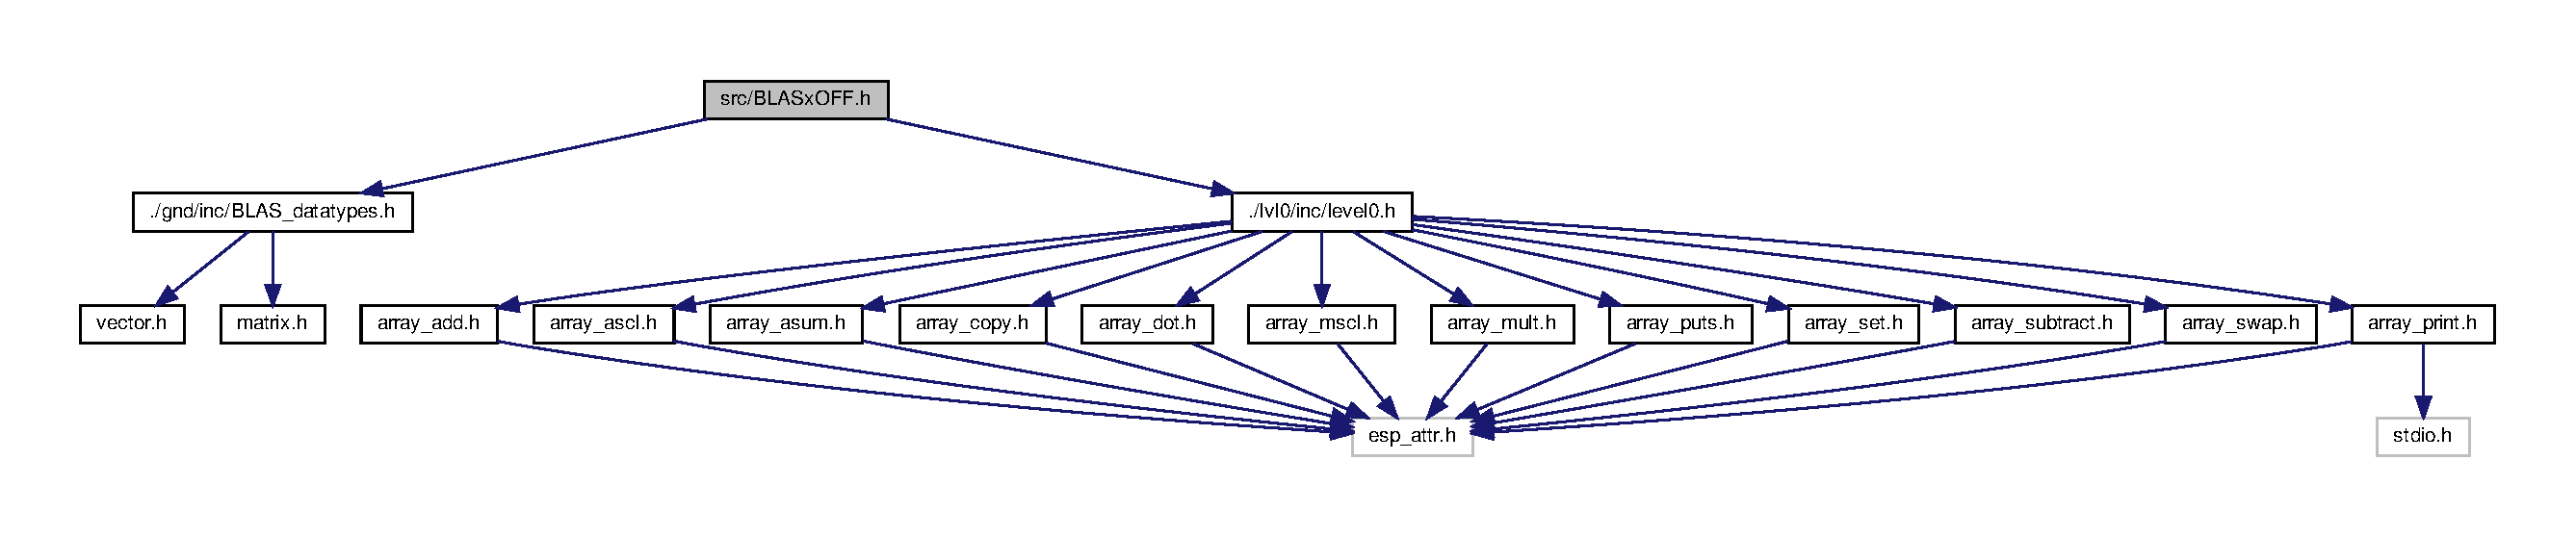
\includegraphics[width=350pt]{BLASxOFF_8h__incl}
\end{center}
\end{figure}

\hypertarget{copy__BLAS_8h}{}\section{src/copy\+\_\+\+B\+L\+AS.h File Reference}
\label{copy__BLAS_8h}\index{src/copy\+\_\+\+B\+L\+A\+S.\+h@{src/copy\+\_\+\+B\+L\+A\+S.\+h}}
{\ttfamily \#include \char`\"{}./gnd/inc/\+B\+L\+A\+S\+\_\+datatypes.\+h\char`\"{}}\newline
{\ttfamily \#include \char`\"{}./lvl0/inc/level0.\+h\char`\"{}}\newline
Include dependency graph for copy\+\_\+\+B\+L\+A\+S.\+h\+:
\nopagebreak
\begin{figure}[H]
\begin{center}
\leavevmode
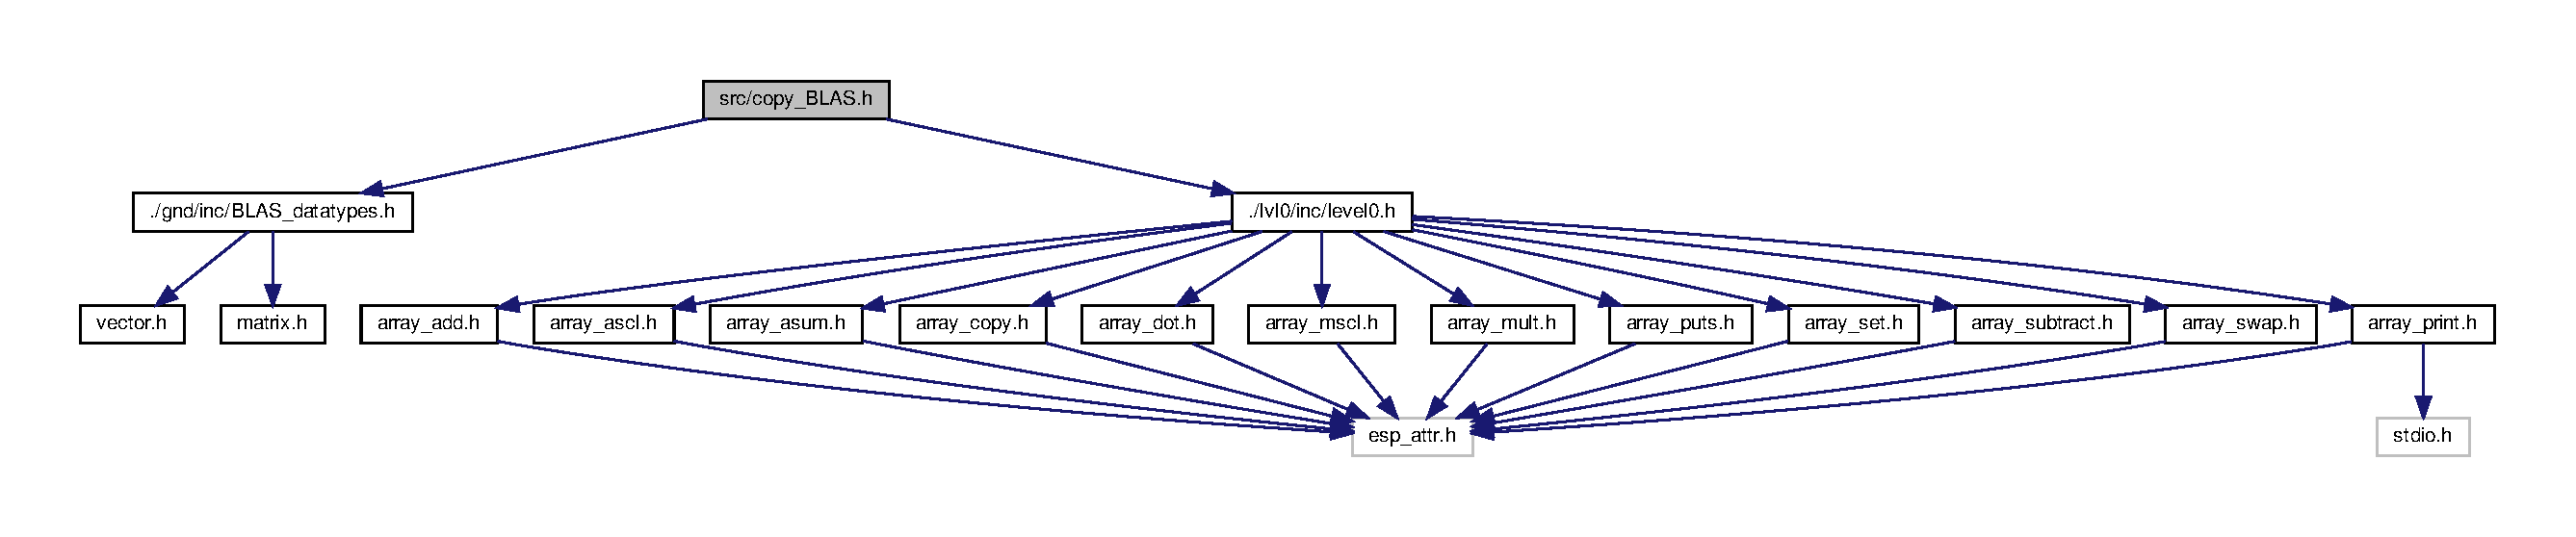
\includegraphics[width=350pt]{copy__BLAS_8h__incl}
\end{center}
\end{figure}

\hypertarget{BLAS__datatypes_8h}{}\section{src/gnd/inc/\+B\+L\+A\+S\+\_\+datatypes.h File Reference}
\label{BLAS__datatypes_8h}\index{src/gnd/inc/\+B\+L\+A\+S\+\_\+datatypes.\+h@{src/gnd/inc/\+B\+L\+A\+S\+\_\+datatypes.\+h}}
{\ttfamily \#include \char`\"{}vector.\+h\char`\"{}}\newline
{\ttfamily \#include \char`\"{}matrix.\+h\char`\"{}}\newline
Include dependency graph for B\+L\+A\+S\+\_\+datatypes.\+h\+:
\nopagebreak
\begin{figure}[H]
\begin{center}
\leavevmode
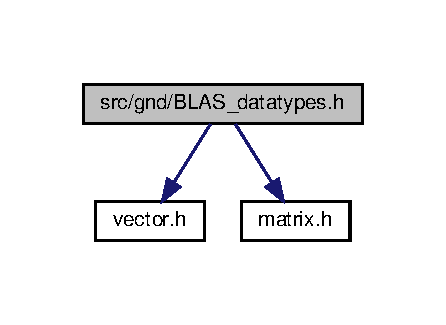
\includegraphics[width=229pt]{BLAS__datatypes_8h__incl}
\end{center}
\end{figure}
This graph shows which files directly or indirectly include this file\+:
\nopagebreak
\begin{figure}[H]
\begin{center}
\leavevmode
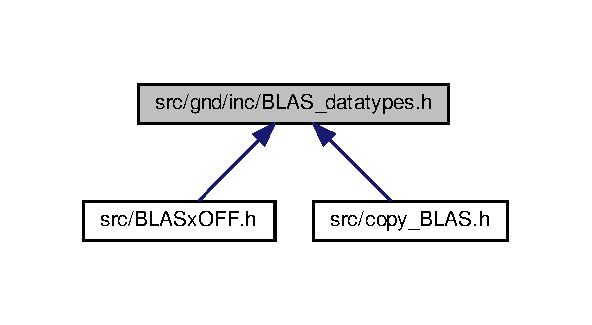
\includegraphics[width=284pt]{BLAS__datatypes_8h__dep__incl}
\end{center}
\end{figure}

\hypertarget{matrix_8h}{}\section{src/gnd/inc/matrix.h File Reference}
\label{matrix_8h}\index{src/gnd/inc/matrix.\+h@{src/gnd/inc/matrix.\+h}}
This graph shows which files directly or indirectly include this file\+:
\nopagebreak
\begin{figure}[H]
\begin{center}
\leavevmode
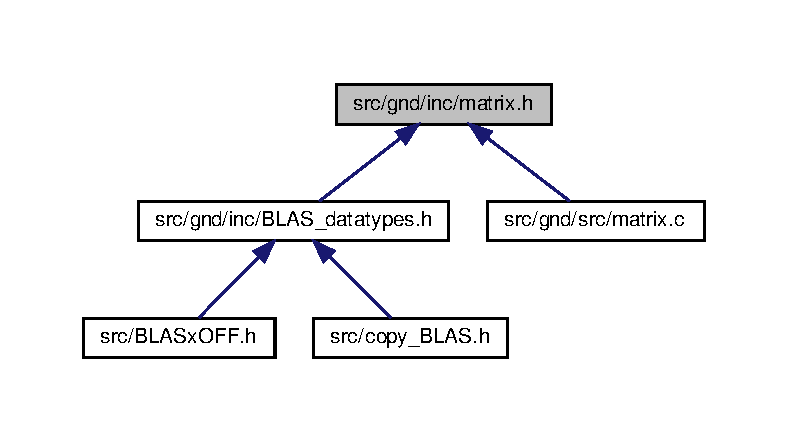
\includegraphics[width=350pt]{matrix_8h__dep__incl}
\end{center}
\end{figure}
\subsection*{Data Structures}
\begin{DoxyCompactItemize}
\item 
struct \hyperlink{structmatrix}{matrix}
\end{DoxyCompactItemize}
\subsection*{Macros}
\begin{DoxyCompactItemize}
\item 
\#define \hyperlink{matrix_8h_ac07aef2092efa03fbc087947d3abcba2}{M\+\_\+\+A\+L\+L\+O\+C\+A\+T\+E\+D\+\_\+F}~1
\begin{DoxyCompactList}\small\item\em Set flag for matrix allocation. \end{DoxyCompactList}\end{DoxyCompactItemize}
\subsection*{Variables}
\begin{DoxyCompactItemize}
\item 
struct \hyperlink{structmatrix}{matrix} \hyperlink{matrix_8h_a11394bf5c56be5e0348b6460f0d04aa0}{new\+\_\+matrix}
\end{DoxyCompactItemize}


\subsection{Macro Definition Documentation}
\mbox{\Hypertarget{matrix_8h_ac07aef2092efa03fbc087947d3abcba2}\label{matrix_8h_ac07aef2092efa03fbc087947d3abcba2}} 
\index{matrix.\+h@{matrix.\+h}!M\+\_\+\+A\+L\+L\+O\+C\+A\+T\+E\+D\+\_\+F@{M\+\_\+\+A\+L\+L\+O\+C\+A\+T\+E\+D\+\_\+F}}
\index{M\+\_\+\+A\+L\+L\+O\+C\+A\+T\+E\+D\+\_\+F@{M\+\_\+\+A\+L\+L\+O\+C\+A\+T\+E\+D\+\_\+F}!matrix.\+h@{matrix.\+h}}
\subsubsection{\texorpdfstring{M\+\_\+\+A\+L\+L\+O\+C\+A\+T\+E\+D\+\_\+F}{M\_ALLOCATED\_F}}
{\footnotesize\ttfamily \#define M\+\_\+\+A\+L\+L\+O\+C\+A\+T\+E\+D\+\_\+F~1}



Set flag for matrix allocation. 

Data type for Matricies used in Linear Algebra 

\subsection{Variable Documentation}
\mbox{\Hypertarget{matrix_8h_a11394bf5c56be5e0348b6460f0d04aa0}\label{matrix_8h_a11394bf5c56be5e0348b6460f0d04aa0}} 
\index{matrix.\+h@{matrix.\+h}!new\+\_\+matrix@{new\+\_\+matrix}}
\index{new\+\_\+matrix@{new\+\_\+matrix}!matrix.\+h@{matrix.\+h}}
\subsubsection{\texorpdfstring{new\+\_\+matrix}{new\_matrix}}
{\footnotesize\ttfamily struct \hyperlink{structmatrix}{matrix} new\+\_\+matrix}

Used to initilize matrix on call

Easy Zero-\/initializer for when making a new matrix 
\hypertarget{vector_8h}{}\section{src/gnd/vector.h File Reference}
\label{vector_8h}\index{src/gnd/vector.\+h@{src/gnd/vector.\+h}}
This graph shows which files directly or indirectly include this file\+:\nopagebreak
\begin{figure}[H]
\begin{center}
\leavevmode
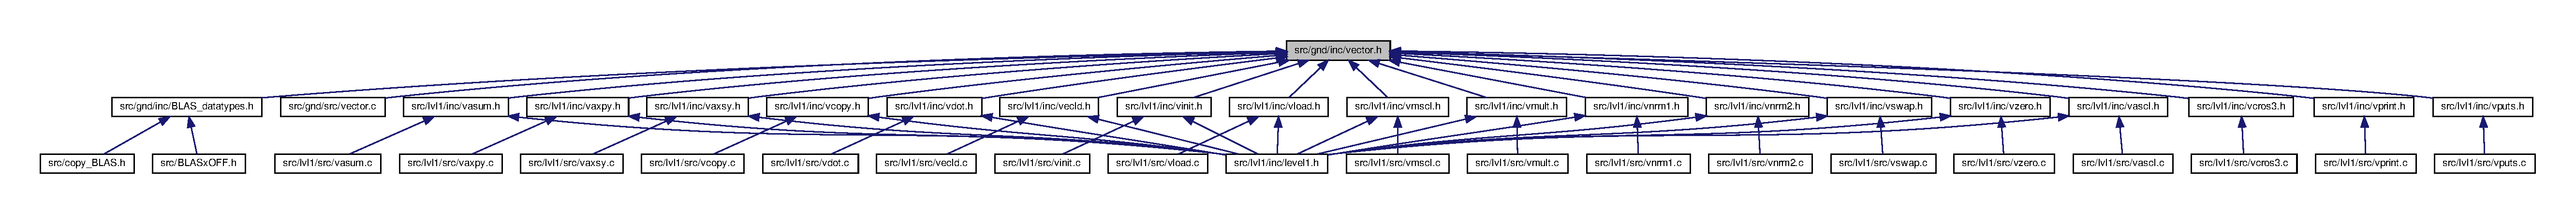
\includegraphics[width=214pt]{vector_8h__dep__incl}
\end{center}
\end{figure}
\subsection*{Data Structures}
\begin{DoxyCompactItemize}
\item 
struct \hyperlink{structvector}{vector}
\end{DoxyCompactItemize}
\subsection*{Macros}
\begin{DoxyCompactItemize}
\item 
\#define \hyperlink{vector_8h_a2566a6db3451171a78842272d28e9373}{V\+\_\+\+A\+L\+L\+O\+C\+A\+T\+E\+D\+\_\+F}~1
\begin{DoxyCompactList}\small\item\em Set flag for vector allocation. \end{DoxyCompactList}\end{DoxyCompactItemize}
\subsection*{Variables}
\begin{DoxyCompactItemize}
\item 
struct \hyperlink{structvector}{vector} \hyperlink{vector_8h_ae0d8044d4d9327f9ecae82ae077e57ea}{new\+\_\+vector}
\end{DoxyCompactItemize}


\subsection{Macro Definition Documentation}
\mbox{\Hypertarget{vector_8h_a2566a6db3451171a78842272d28e9373}\label{vector_8h_a2566a6db3451171a78842272d28e9373}} 
\index{vector.\+h@{vector.\+h}!V\+\_\+\+A\+L\+L\+O\+C\+A\+T\+E\+D\+\_\+F@{V\+\_\+\+A\+L\+L\+O\+C\+A\+T\+E\+D\+\_\+F}}
\index{V\+\_\+\+A\+L\+L\+O\+C\+A\+T\+E\+D\+\_\+F@{V\+\_\+\+A\+L\+L\+O\+C\+A\+T\+E\+D\+\_\+F}!vector.\+h@{vector.\+h}}
\subsubsection{\texorpdfstring{V\+\_\+\+A\+L\+L\+O\+C\+A\+T\+E\+D\+\_\+F}{V\_ALLOCATED\_F}}
{\footnotesize\ttfamily \#define V\+\_\+\+A\+L\+L\+O\+C\+A\+T\+E\+D\+\_\+F~1}



Set flag for vector allocation. 

Data type for Vatricies used in Linear Algebra 

\subsection{Variable Documentation}
\mbox{\Hypertarget{vector_8h_ae0d8044d4d9327f9ecae82ae077e57ea}\label{vector_8h_ae0d8044d4d9327f9ecae82ae077e57ea}} 
\index{vector.\+h@{vector.\+h}!new\+\_\+vector@{new\+\_\+vector}}
\index{new\+\_\+vector@{new\+\_\+vector}!vector.\+h@{vector.\+h}}
\subsubsection{\texorpdfstring{new\+\_\+vector}{new\_vector}}
{\footnotesize\ttfamily struct \hyperlink{structvector}{vector} new\+\_\+vector}

Used to initilize vector on call

Easy Zero-\/initializer for when making a new matrix 
\hypertarget{gnd_2inc_2vinit_8h}{}\section{src/gnd/inc/vinit.h File Reference}
\label{gnd_2inc_2vinit_8h}\index{src/gnd/inc/vinit.\+h@{src/gnd/inc/vinit.\+h}}
{\ttfamily \#include \char`\"{}esp\+\_\+attr.\+h\char`\"{}}\newline
{\ttfamily \#include \char`\"{}vector.\+h\char`\"{}}\newline
Include dependency graph for vinit.\+h\+:
\nopagebreak
\begin{figure}[H]
\begin{center}
\leavevmode
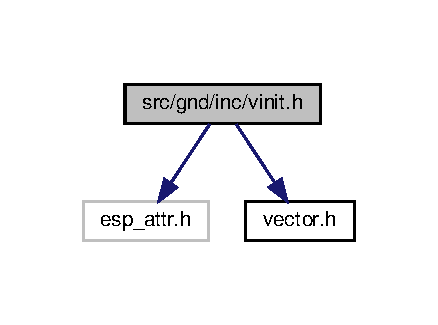
\includegraphics[width=210pt]{gnd_2inc_2vinit_8h__incl}
\end{center}
\end{figure}
This graph shows which files directly or indirectly include this file\+:
\nopagebreak
\begin{figure}[H]
\begin{center}
\leavevmode
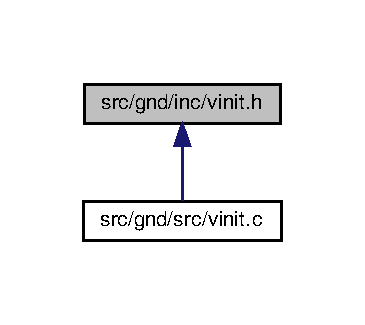
\includegraphics[width=175pt]{gnd_2inc_2vinit_8h__dep__incl}
\end{center}
\end{figure}
\subsection*{Functions}
\begin{DoxyCompactItemize}
\item 
int I\+R\+A\+M\+\_\+\+A\+T\+TR \hyperlink{gnd_2inc_2vinit_8h_adaa2b99da82281a924f974a6c0ee48a5}{vinit} (struct \hyperlink{structvector}{vector} $\ast$V, const unsigned int l) \hyperlink{array__zero_8h_a773bfa726d26ed3aba89b686193787aa}{\+\_\+\+\_\+attribute\+\_\+\+\_\+}((nonull))
\end{DoxyCompactItemize}


\subsection{Function Documentation}
\mbox{\Hypertarget{gnd_2inc_2vinit_8h_adaa2b99da82281a924f974a6c0ee48a5}\label{gnd_2inc_2vinit_8h_adaa2b99da82281a924f974a6c0ee48a5}} 
\index{gnd/inc/vinit.\+h@{gnd/inc/vinit.\+h}!vinit@{vinit}}
\index{vinit@{vinit}!gnd/inc/vinit.\+h@{gnd/inc/vinit.\+h}}
\subsubsection{\texorpdfstring{vinit()}{vinit()}}
{\footnotesize\ttfamily int I\+R\+A\+M\+\_\+\+A\+T\+TR vinit (\begin{DoxyParamCaption}\item[{struct \hyperlink{structvector}{vector} $\ast$}]{V,  }\item[{const unsigned int}]{l }\end{DoxyParamCaption})}

Utitility function for initializing vector datatypes

Return Codes 0 $\sim$ Vector Initialization and Allocation was successful -\/1 $\sim$ (E\+R\+R\+OR) Vector has already been initialized -\/2 $\sim$ (E\+R\+R\+OR) Malloc has failed 
\hypertarget{lvl1_2inc_2vinit_8h}{}\section{src/lvl1/inc/vinit.h File Reference}
\label{lvl1_2inc_2vinit_8h}\index{src/lvl1/inc/vinit.\+h@{src/lvl1/inc/vinit.\+h}}
{\ttfamily \#include \char`\"{}esp\+\_\+attr.\+h\char`\"{}}\newline
{\ttfamily \#include \char`\"{}../../gnd/inc/vector.\+h\char`\"{}}\newline
Include dependency graph for vinit.\+h\+:
\nopagebreak
\begin{figure}[H]
\begin{center}
\leavevmode
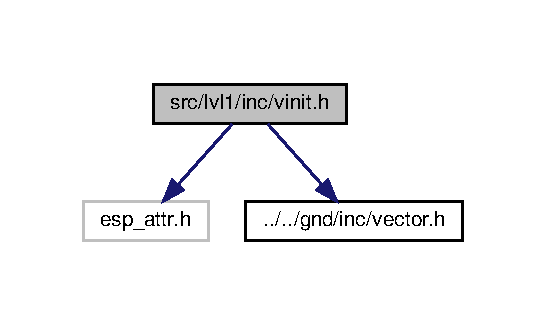
\includegraphics[width=262pt]{lvl1_2inc_2vinit_8h__incl}
\end{center}
\end{figure}
This graph shows which files directly or indirectly include this file\+:
\nopagebreak
\begin{figure}[H]
\begin{center}
\leavevmode
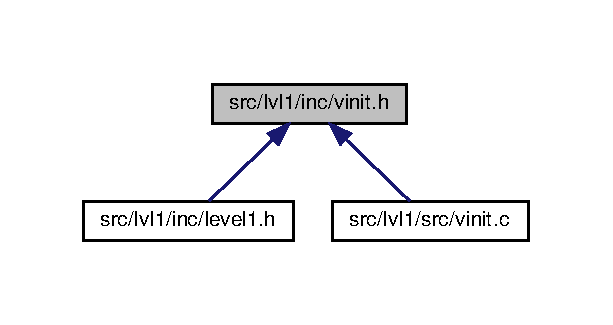
\includegraphics[width=294pt]{lvl1_2inc_2vinit_8h__dep__incl}
\end{center}
\end{figure}
\subsection*{Functions}
\begin{DoxyCompactItemize}
\item 
int I\+R\+A\+M\+\_\+\+A\+T\+TR \hyperlink{lvl1_2inc_2vinit_8h_adaa2b99da82281a924f974a6c0ee48a5}{vinit} (struct \hyperlink{structvector}{vector} $\ast$V, const unsigned int l) \hyperlink{array__zero_8h_a773bfa726d26ed3aba89b686193787aa}{\+\_\+\+\_\+attribute\+\_\+\+\_\+}((nonull))
\end{DoxyCompactItemize}


\subsection{Function Documentation}
\mbox{\Hypertarget{lvl1_2inc_2vinit_8h_adaa2b99da82281a924f974a6c0ee48a5}\label{lvl1_2inc_2vinit_8h_adaa2b99da82281a924f974a6c0ee48a5}} 
\index{lvl1/inc/vinit.\+h@{lvl1/inc/vinit.\+h}!vinit@{vinit}}
\index{vinit@{vinit}!lvl1/inc/vinit.\+h@{lvl1/inc/vinit.\+h}}
\subsubsection{\texorpdfstring{vinit()}{vinit()}}
{\footnotesize\ttfamily int I\+R\+A\+M\+\_\+\+A\+T\+TR vinit (\begin{DoxyParamCaption}\item[{struct \hyperlink{structvector}{vector} $\ast$}]{V,  }\item[{const unsigned int}]{l }\end{DoxyParamCaption})}

Utitility function for initializing vector datatypes

Return Codes 0 $\sim$ Vector Initialization and Allocation was successful -\/1 $\sim$ (E\+R\+R\+OR) Vector has already been initialized -\/2 $\sim$ (E\+R\+R\+OR) Malloc has failed 
\hypertarget{matrix_8c}{}\section{src/gnd/src/matrix.c File Reference}
\label{matrix_8c}\index{src/gnd/src/matrix.\+c@{src/gnd/src/matrix.\+c}}
{\ttfamily \#include $<$stddef.\+h$>$}\newline
{\ttfamily \#include \char`\"{}../inc/matrix.\+h\char`\"{}}\newline
Include dependency graph for matrix.\+c\+:\nopagebreak
\begin{figure}[H]
\begin{center}
\leavevmode
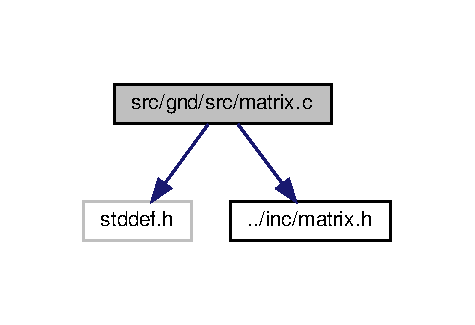
\includegraphics[width=228pt]{matrix_8c__incl}
\end{center}
\end{figure}
\subsection*{Variables}
\begin{DoxyCompactItemize}
\item 
struct \hyperlink{structmatrix}{matrix} \hyperlink{matrix_8c_a11394bf5c56be5e0348b6460f0d04aa0}{new\+\_\+matrix}
\end{DoxyCompactItemize}


\subsection{Variable Documentation}
\mbox{\Hypertarget{matrix_8c_a11394bf5c56be5e0348b6460f0d04aa0}\label{matrix_8c_a11394bf5c56be5e0348b6460f0d04aa0}} 
\index{matrix.\+c@{matrix.\+c}!new\+\_\+matrix@{new\+\_\+matrix}}
\index{new\+\_\+matrix@{new\+\_\+matrix}!matrix.\+c@{matrix.\+c}}
\subsubsection{\texorpdfstring{new\+\_\+matrix}{new\_matrix}}
{\footnotesize\ttfamily struct \hyperlink{structmatrix}{matrix} new\+\_\+matrix}

{\bfseries Initial value\+:}
\begin{DoxyCode}
= \{
  .flags = 0,
  .r = 0,
  .c = 0,
  .l = 0,
  .name = NULL,
  .m = NULL,
\}
\end{DoxyCode}
Easy Zero-\/initializer for when making a new matrix 
\hypertarget{vector_8c}{}\section{src/gnd/src/vector.c File Reference}
\label{vector_8c}\index{src/gnd/src/vector.\+c@{src/gnd/src/vector.\+c}}
{\ttfamily \#include $<$stddef.\+h$>$}\newline
{\ttfamily \#include \char`\"{}../inc/vector.\+h\char`\"{}}\newline
Include dependency graph for vector.\+c\+:\nopagebreak
\begin{figure}[H]
\begin{center}
\leavevmode
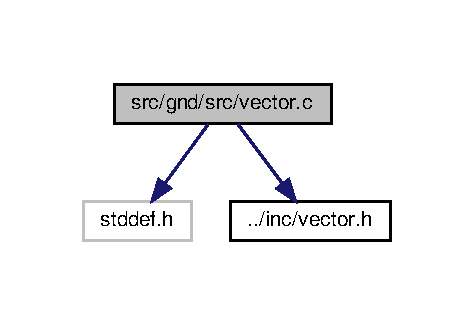
\includegraphics[width=228pt]{vector_8c__incl}
\end{center}
\end{figure}
\subsection*{Variables}
\begin{DoxyCompactItemize}
\item 
struct \hyperlink{structvector}{vector} \hyperlink{vector_8c_ae0d8044d4d9327f9ecae82ae077e57ea}{new\+\_\+vector}
\end{DoxyCompactItemize}


\subsection{Variable Documentation}
\mbox{\Hypertarget{vector_8c_ae0d8044d4d9327f9ecae82ae077e57ea}\label{vector_8c_ae0d8044d4d9327f9ecae82ae077e57ea}} 
\index{vector.\+c@{vector.\+c}!new\+\_\+vector@{new\+\_\+vector}}
\index{new\+\_\+vector@{new\+\_\+vector}!vector.\+c@{vector.\+c}}
\subsubsection{\texorpdfstring{new\+\_\+vector}{new\_vector}}
{\footnotesize\ttfamily struct \hyperlink{structvector}{vector} new\+\_\+vector}

{\bfseries Initial value\+:}
\begin{DoxyCode}
= \{
  .flags = 0,
  .l = 0,
  .v = NULL,
\}
\end{DoxyCode}
Easy Zero-\/initializer for when making a new matrix 
\hypertarget{gnd_2src_2vinit_8c}{}\section{src/gnd/src/vinit.c File Reference}
\label{gnd_2src_2vinit_8c}\index{src/gnd/src/vinit.\+c@{src/gnd/src/vinit.\+c}}
{\ttfamily \#include \char`\"{}../inc/vinit.\+h\char`\"{}}\newline
{\ttfamily \#include $<$stddef.\+h$>$}\newline
{\ttfamily \#include $<$stdlib.\+h$>$}\newline
Include dependency graph for vinit.\+c\+:
\nopagebreak
\begin{figure}[H]
\begin{center}
\leavevmode
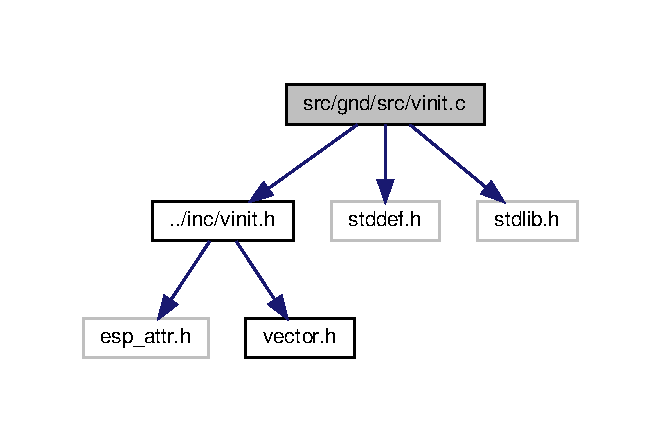
\includegraphics[width=317pt]{gnd_2src_2vinit_8c__incl}
\end{center}
\end{figure}
\subsection*{Functions}
\begin{DoxyCompactItemize}
\item 
int \hyperlink{gnd_2src_2vinit_8c_a18333d150d08e8d04f2d9cf71ec2141f}{vinit} (struct \hyperlink{structvector}{vector} $\ast$V, const unsigned int l)
\end{DoxyCompactItemize}


\subsection{Function Documentation}
\mbox{\Hypertarget{gnd_2src_2vinit_8c_a18333d150d08e8d04f2d9cf71ec2141f}\label{gnd_2src_2vinit_8c_a18333d150d08e8d04f2d9cf71ec2141f}} 
\index{gnd/src/vinit.\+c@{gnd/src/vinit.\+c}!vinit@{vinit}}
\index{vinit@{vinit}!gnd/src/vinit.\+c@{gnd/src/vinit.\+c}}
\subsubsection{\texorpdfstring{vinit()}{vinit()}}
{\footnotesize\ttfamily int vinit (\begin{DoxyParamCaption}\item[{struct \hyperlink{structvector}{vector} $\ast$}]{V,  }\item[{const unsigned int}]{l }\end{DoxyParamCaption})}

Utitility function for initializing vector datatypes

Return Codes 0 $\sim$ Vector Initialization and Allocation was successful -\/1 $\sim$ (E\+R\+R\+OR) Vector has already been initialized -\/2 $\sim$ (E\+R\+R\+OR) Malloc has failed 
\hypertarget{lvl1_2src_2vinit_8c}{}\section{src/lvl1/src/vinit.c File Reference}
\label{lvl1_2src_2vinit_8c}\index{src/lvl1/src/vinit.\+c@{src/lvl1/src/vinit.\+c}}
{\ttfamily \#include \char`\"{}../inc/vinit.\+h\char`\"{}}\newline
{\ttfamily \#include $<$stddef.\+h$>$}\newline
{\ttfamily \#include $<$stdlib.\+h$>$}\newline
Include dependency graph for vinit.\+c\+:
\nopagebreak
\begin{figure}[H]
\begin{center}
\leavevmode
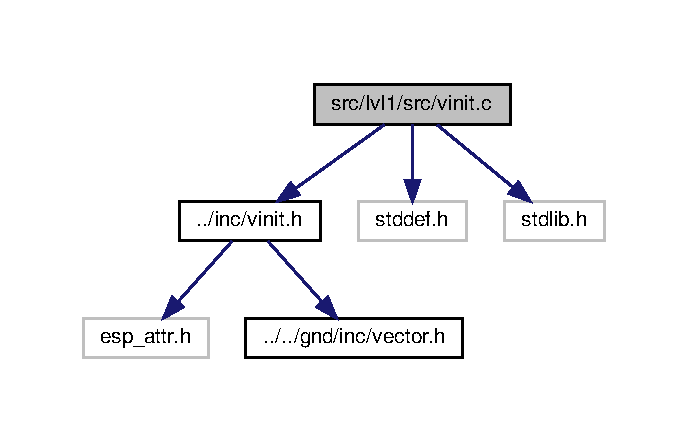
\includegraphics[width=330pt]{lvl1_2src_2vinit_8c__incl}
\end{center}
\end{figure}
\subsection*{Functions}
\begin{DoxyCompactItemize}
\item 
int \hyperlink{lvl1_2src_2vinit_8c_a18333d150d08e8d04f2d9cf71ec2141f}{vinit} (struct \hyperlink{structvector}{vector} $\ast$V, const unsigned int l)
\end{DoxyCompactItemize}


\subsection{Function Documentation}
\mbox{\Hypertarget{lvl1_2src_2vinit_8c_a18333d150d08e8d04f2d9cf71ec2141f}\label{lvl1_2src_2vinit_8c_a18333d150d08e8d04f2d9cf71ec2141f}} 
\index{lvl1/src/vinit.\+c@{lvl1/src/vinit.\+c}!vinit@{vinit}}
\index{vinit@{vinit}!lvl1/src/vinit.\+c@{lvl1/src/vinit.\+c}}
\subsubsection{\texorpdfstring{vinit()}{vinit()}}
{\footnotesize\ttfamily int vinit (\begin{DoxyParamCaption}\item[{struct \hyperlink{structvector}{vector} $\ast$}]{V,  }\item[{const unsigned int}]{l }\end{DoxyParamCaption})}

Utitility function for initializing vector datatypes

Return Codes 0 $\sim$ Vector Initialization and Allocation was successful -\/1 $\sim$ (E\+R\+R\+OR) Vector has already been initialized -\/2 $\sim$ (E\+R\+R\+OR) Malloc has failed 
\hypertarget{array__add_8h}{}\section{src/lvl0/inc/array\+\_\+add.h File Reference}
\label{array__add_8h}\index{src/lvl0/inc/array\+\_\+add.\+h@{src/lvl0/inc/array\+\_\+add.\+h}}
{\ttfamily \#include \char`\"{}esp\+\_\+attr.\+h\char`\"{}}\newline
{\ttfamily \#include \char`\"{}../src/array\+\_\+add.\+c\char`\"{}}\newline
Include dependency graph for array\+\_\+add.\+h\+:\nopagebreak
\begin{figure}[H]
\begin{center}
\leavevmode
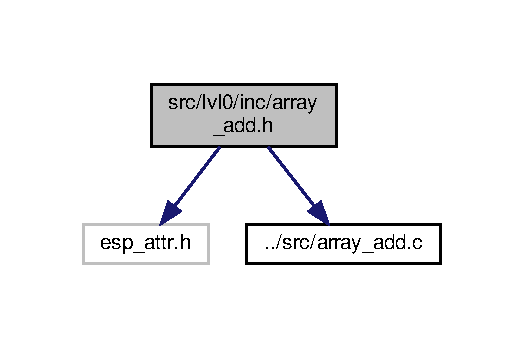
\includegraphics[width=252pt]{array__add_8h__incl}
\end{center}
\end{figure}
This graph shows which files directly or indirectly include this file\+:
\nopagebreak
\begin{figure}[H]
\begin{center}
\leavevmode
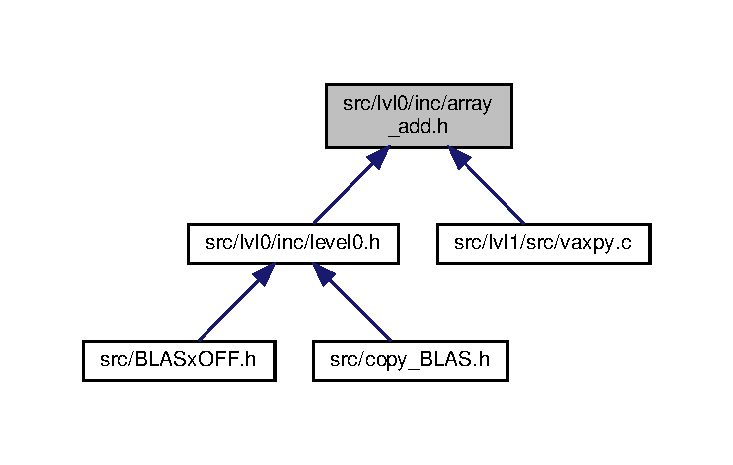
\includegraphics[width=284pt]{array__add_8h__dep__incl}
\end{center}
\end{figure}
\subsection*{Functions}
\begin{DoxyCompactItemize}
\item 
void I\+R\+A\+M\+\_\+\+A\+T\+TR \hyperlink{array__add_8h_a15b992b0dbde8612a35532df8efd7b4d}{array\+\_\+add} (float $\ast$arr\+Res, const float $\ast$arr\+OprA, const float $\ast$arr\+OprB, const unsigned int start, const unsigned int end) \+\_\+\+\_\+attribute\+\_\+\+\_\+((always\+\_\+inline)) \+\_\+\+\_\+attribute\+\_\+\+\_\+((nonull))
\end{DoxyCompactItemize}


\subsection{Function Documentation}
\mbox{\Hypertarget{array__add_8h_a15b992b0dbde8612a35532df8efd7b4d}\label{array__add_8h_a15b992b0dbde8612a35532df8efd7b4d}} 
\index{array\+\_\+add.\+h@{array\+\_\+add.\+h}!array\+\_\+add@{array\+\_\+add}}
\index{array\+\_\+add@{array\+\_\+add}!array\+\_\+add.\+h@{array\+\_\+add.\+h}}
\subsubsection{\texorpdfstring{array\+\_\+add()}{array\_add()}}
{\footnotesize\ttfamily void I\+R\+A\+M\+\_\+\+A\+T\+TR array\+\_\+add (\begin{DoxyParamCaption}\item[{float $\ast$}]{arr\+Res,  }\item[{const float $\ast$}]{arr\+OprA,  }\item[{const float $\ast$}]{arr\+OprB,  }\item[{const unsigned int}]{start,  }\item[{const unsigned int}]{end }\end{DoxyParamCaption})}

This function add two arrays together element by element 
\begin{DoxyParams}{Parameters}
{\em arr\+Res} & Array pointer where the result will be stored \\
\hline
{\em arr\+OprA} & Array pointer for the 1st operand \\
\hline
{\em arr\+OprB} & Array pointer for the 2nd operand \\
\hline
{\em start} & Starting element index to loop across \\
\hline
{\em end} & Last element index to loop across \\
\hline
\end{DoxyParams}

\hypertarget{array__ascl_8h}{}\section{src/lvl0/inc/array\+\_\+ascl.h File Reference}
\label{array__ascl_8h}\index{src/lvl0/inc/array\+\_\+ascl.\+h@{src/lvl0/inc/array\+\_\+ascl.\+h}}
{\ttfamily \#include \char`\"{}esp\+\_\+attr.\+h\char`\"{}}\newline
Include dependency graph for array\+\_\+ascl.\+h\+:
\nopagebreak
\begin{figure}[H]
\begin{center}
\leavevmode
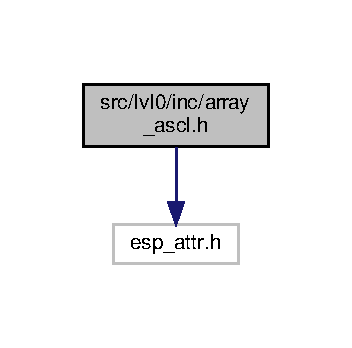
\includegraphics[width=169pt]{array__ascl_8h__incl}
\end{center}
\end{figure}
This graph shows which files directly or indirectly include this file\+:
\nopagebreak
\begin{figure}[H]
\begin{center}
\leavevmode
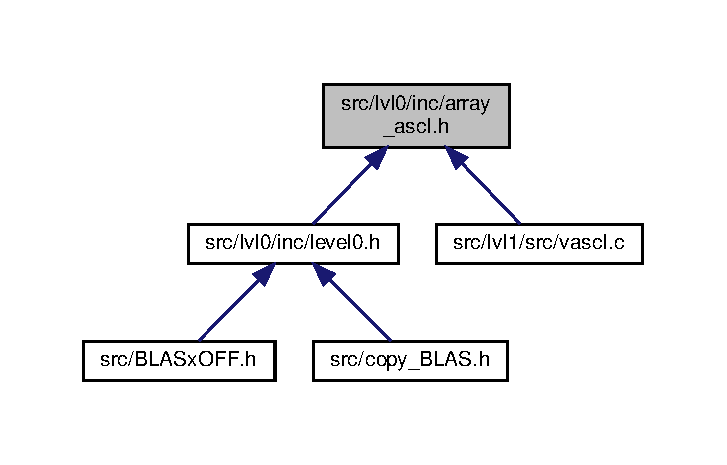
\includegraphics[width=349pt]{array__ascl_8h__dep__incl}
\end{center}
\end{figure}
\subsection*{Functions}
\begin{DoxyCompactItemize}
\item 
void I\+R\+A\+M\+\_\+\+A\+T\+TR \hyperlink{array__ascl_8h_a2cd5fcee5a0a6d5d582583da1daa095b}{\+\_\+\+\_\+attribute\+\_\+\+\_\+} ((always\+\_\+inline)) \+\_\+\+\_\+attribute\+\_\+\+\_\+((nonull)) array\+\_\+ascl(float $\ast$arr\+Res
\end{DoxyCompactItemize}
\subsection*{Variables}
\begin{DoxyCompactItemize}
\item 
void I\+R\+A\+M\+\_\+\+A\+T\+TR const float $\ast$ \hyperlink{array__ascl_8h_a951b57ce1d7dd691d9a66eda776f43f6}{arr\+Opr}
\begin{DoxyCompactList}\small\item\em $<$ Array pointer where the result will be stored \end{DoxyCompactList}\item 
void I\+R\+A\+M\+\_\+\+A\+T\+TR const float const float \hyperlink{array__ascl_8h_a8beac99f3a0446385106d145d3de1f90}{scl\+Opr}
\begin{DoxyCompactList}\small\item\em Scalar operand to add to the elements of the array operand. \end{DoxyCompactList}\item 
void I\+R\+A\+M\+\_\+\+A\+T\+TR const float const float const unsigned int \hyperlink{array__ascl_8h_a0549b2187026de7f72c6b3214fa437d5}{start}
\begin{DoxyCompactList}\small\item\em Begining element index to begin loop. \end{DoxyCompactList}\item 
void I\+R\+A\+M\+\_\+\+A\+T\+TR const float const float const unsigned int const unsigned int \hyperlink{array__ascl_8h_a68c28899964e31626b3c9e42853f0d42}{end}
\begin{DoxyCompactList}\small\item\em $<$ Last element index to loop across \end{DoxyCompactList}\end{DoxyCompactItemize}


\subsection{Function Documentation}
\mbox{\Hypertarget{array__ascl_8h_a2cd5fcee5a0a6d5d582583da1daa095b}\label{array__ascl_8h_a2cd5fcee5a0a6d5d582583da1daa095b}} 
\index{array\+\_\+ascl.\+h@{array\+\_\+ascl.\+h}!\+\_\+\+\_\+attribute\+\_\+\+\_\+@{\+\_\+\+\_\+attribute\+\_\+\+\_\+}}
\index{\+\_\+\+\_\+attribute\+\_\+\+\_\+@{\+\_\+\+\_\+attribute\+\_\+\+\_\+}!array\+\_\+ascl.\+h@{array\+\_\+ascl.\+h}}
\subsubsection{\texorpdfstring{\+\_\+\+\_\+attribute\+\_\+\+\_\+()}{\_\_attribute\_\_()}}
{\footnotesize\ttfamily void I\+R\+A\+M\+\_\+\+A\+T\+TR \+\_\+\+\_\+attribute\+\_\+\+\_\+ (\begin{DoxyParamCaption}\item[{(always\+\_\+inline)}]{ }\end{DoxyParamCaption})\hspace{0.3cm}{\ttfamily [inline]}}

This function adds a scalar too each element in an array


\begin{DoxyItemize}
\item This function is deliberatly placed in Instruction R\+AM. Meaning that this function will always remained cached.
\item the {\bfseries attribute}((always\+\_\+inline)) tells the compiler to A\+L\+W\+A\+YS inline to function reguardless of optimization levels
\item the {\bfseries attribute}((nonull)) tells the compiler that the function\textquotesingle{}s pointer arguments cannot bell N\+U\+LL 
\end{DoxyItemize}

\subsection{Variable Documentation}
\mbox{\Hypertarget{array__ascl_8h_a951b57ce1d7dd691d9a66eda776f43f6}\label{array__ascl_8h_a951b57ce1d7dd691d9a66eda776f43f6}} 
\index{array\+\_\+ascl.\+h@{array\+\_\+ascl.\+h}!arr\+Opr@{arr\+Opr}}
\index{arr\+Opr@{arr\+Opr}!array\+\_\+ascl.\+h@{array\+\_\+ascl.\+h}}
\subsubsection{\texorpdfstring{arr\+Opr}{arrOpr}}
{\footnotesize\ttfamily void I\+R\+A\+M\+\_\+\+A\+T\+TR const float$\ast$ arr\+Opr}



$<$ Array pointer where the result will be stored 

Pointer for the array operand \mbox{\Hypertarget{array__ascl_8h_a68c28899964e31626b3c9e42853f0d42}\label{array__ascl_8h_a68c28899964e31626b3c9e42853f0d42}} 
\index{array\+\_\+ascl.\+h@{array\+\_\+ascl.\+h}!end@{end}}
\index{end@{end}!array\+\_\+ascl.\+h@{array\+\_\+ascl.\+h}}
\subsubsection{\texorpdfstring{end}{end}}
{\footnotesize\ttfamily void I\+R\+A\+M\+\_\+\+A\+T\+TR const float const float const unsigned int const unsigned int end}

{\bfseries Initial value\+:}
\begin{DoxyCode}
\{
    \textcolor{keywordflow}{for}(\textcolor{keywordtype}{unsigned} \textcolor{keywordtype}{int} I=\hyperlink{array__ascl_8h_a0549b2187026de7f72c6b3214fa437d5}{start}; I<\hyperlink{array__ascl_8h_a68c28899964e31626b3c9e42853f0d42}{end};++I) \{
      arrRes[I] = \hyperlink{array__ascl_8h_a951b57ce1d7dd691d9a66eda776f43f6}{arrOpr}[I] + \hyperlink{array__ascl_8h_a8beac99f3a0446385106d145d3de1f90}{sclOpr};
    \}
    \textcolor{keywordflow}{return}
\end{DoxyCode}


$<$ Last element index to loop across 

\mbox{\Hypertarget{array__ascl_8h_a8beac99f3a0446385106d145d3de1f90}\label{array__ascl_8h_a8beac99f3a0446385106d145d3de1f90}} 
\index{array\+\_\+ascl.\+h@{array\+\_\+ascl.\+h}!scl\+Opr@{scl\+Opr}}
\index{scl\+Opr@{scl\+Opr}!array\+\_\+ascl.\+h@{array\+\_\+ascl.\+h}}
\subsubsection{\texorpdfstring{scl\+Opr}{sclOpr}}
{\footnotesize\ttfamily void I\+R\+A\+M\+\_\+\+A\+T\+TR const float const float scl\+Opr}



Scalar operand to add to the elements of the array operand. 

\mbox{\Hypertarget{array__ascl_8h_a0549b2187026de7f72c6b3214fa437d5}\label{array__ascl_8h_a0549b2187026de7f72c6b3214fa437d5}} 
\index{array\+\_\+ascl.\+h@{array\+\_\+ascl.\+h}!start@{start}}
\index{start@{start}!array\+\_\+ascl.\+h@{array\+\_\+ascl.\+h}}
\subsubsection{\texorpdfstring{start}{start}}
{\footnotesize\ttfamily void I\+R\+A\+M\+\_\+\+A\+T\+TR const float const float const unsigned int start}



Begining element index to begin loop. 


\hypertarget{array__asum_8h}{}\section{src/lvl0/inc/array\+\_\+asum.h File Reference}
\label{array__asum_8h}\index{src/lvl0/inc/array\+\_\+asum.\+h@{src/lvl0/inc/array\+\_\+asum.\+h}}
{\ttfamily \#include \char`\"{}esp\+\_\+attr.\+h\char`\"{}}\newline
Include dependency graph for array\+\_\+asum.\+h\+:
\nopagebreak
\begin{figure}[H]
\begin{center}
\leavevmode
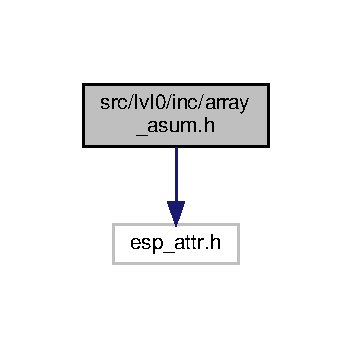
\includegraphics[width=169pt]{array__asum_8h__incl}
\end{center}
\end{figure}
This graph shows which files directly or indirectly include this file\+:
\nopagebreak
\begin{figure}[H]
\begin{center}
\leavevmode
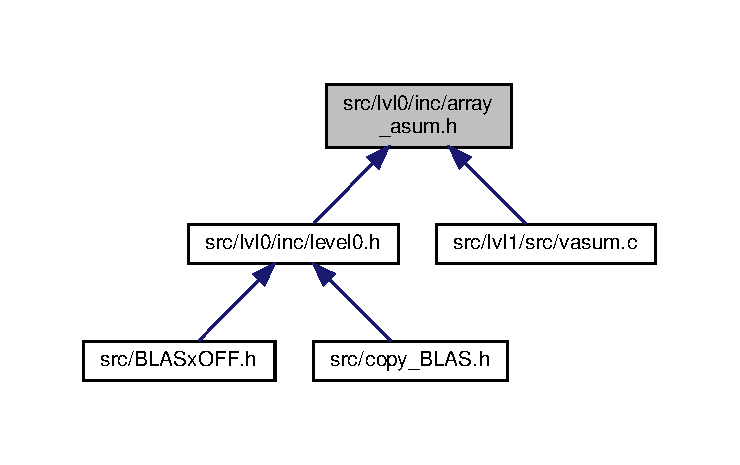
\includegraphics[width=350pt]{array__asum_8h__dep__incl}
\end{center}
\end{figure}
\subsection*{Functions}
\begin{DoxyCompactItemize}
\item 
void I\+R\+A\+M\+\_\+\+A\+T\+TR \hyperlink{array__asum_8h_af8fe767b6255bf4e9260b478c555a44f}{\+\_\+\+\_\+attribute\+\_\+\+\_\+} ((always\+\_\+inline)) \+\_\+\+\_\+attribute\+\_\+\+\_\+((nonull)) array\+\_\+asum(float $\ast$\hyperlink{array__dot_8h_a679c62e32495a27559a1723609a78a20}{scl\+Res}
\item 
\hyperlink{array__asum_8h_abe37ef39291fe27f977e30e3118c90f9}{for} (unsigned int I=\hyperlink{array__zero_8h_a1951879481f1ba4287d30b0a485429fc}{start};I$<$ \hyperlink{array__zero_8h_ae062d39ef5523e038e43c08fa9fe07b4}{end};++I)
\end{DoxyCompactItemize}
\subsection*{Variables}
\begin{DoxyCompactItemize}
\item 
void I\+R\+A\+M\+\_\+\+A\+T\+TR const float $\ast$ \hyperlink{array__asum_8h_a951b57ce1d7dd691d9a66eda776f43f6}{arr\+Opr}
\begin{DoxyCompactList}\small\item\em $<$ Float pointer for return value \end{DoxyCompactList}\item 
void I\+R\+A\+M\+\_\+\+A\+T\+TR const float const unsigned int \hyperlink{array__asum_8h_afd423ccb9a3b73eaf00854e74324938e}{start}
\begin{DoxyCompactList}\small\item\em Starting element index to loop across. \end{DoxyCompactList}\item 
void I\+R\+A\+M\+\_\+\+A\+T\+TR const float const unsigned int const unsigned int \hyperlink{array__asum_8h_a3827eeafb6094da9458f36d58f5e1f8e}{end}
\begin{DoxyCompactList}\small\item\em $<$ Last element index to loop across \end{DoxyCompactList}\item 
$\ast$ \hyperlink{array__asum_8h_a679c62e32495a27559a1723609a78a20}{scl\+Res} = res
\item 
\hyperlink{array__asum_8h_a9717e7bbecb906637e86cef6da3d83c2}{return}
\end{DoxyCompactItemize}


\subsection{Function Documentation}
\mbox{\Hypertarget{array__asum_8h_af8fe767b6255bf4e9260b478c555a44f}\label{array__asum_8h_af8fe767b6255bf4e9260b478c555a44f}} 
\index{array\+\_\+asum.\+h@{array\+\_\+asum.\+h}!\+\_\+\+\_\+attribute\+\_\+\+\_\+@{\+\_\+\+\_\+attribute\+\_\+\+\_\+}}
\index{\+\_\+\+\_\+attribute\+\_\+\+\_\+@{\+\_\+\+\_\+attribute\+\_\+\+\_\+}!array\+\_\+asum.\+h@{array\+\_\+asum.\+h}}
\subsubsection{\texorpdfstring{\+\_\+\+\_\+attribute\+\_\+\+\_\+()}{\_\_attribute\_\_()}}
{\footnotesize\ttfamily void I\+R\+A\+M\+\_\+\+A\+T\+TR \+\_\+\+\_\+attribute\+\_\+\+\_\+ (\begin{DoxyParamCaption}\item[{(always\+\_\+inline)}]{ }\end{DoxyParamCaption})\hspace{0.3cm}{\ttfamily [inline]}}

This function adds all the elements in an array and returns the sum \mbox{\Hypertarget{array__asum_8h_abe37ef39291fe27f977e30e3118c90f9}\label{array__asum_8h_abe37ef39291fe27f977e30e3118c90f9}} 
\index{array\+\_\+asum.\+h@{array\+\_\+asum.\+h}!for@{for}}
\index{for@{for}!array\+\_\+asum.\+h@{array\+\_\+asum.\+h}}
\subsubsection{\texorpdfstring{for()}{for()}}
{\footnotesize\ttfamily for (\begin{DoxyParamCaption}{ }\end{DoxyParamCaption})}



\subsection{Variable Documentation}
\mbox{\Hypertarget{array__asum_8h_a951b57ce1d7dd691d9a66eda776f43f6}\label{array__asum_8h_a951b57ce1d7dd691d9a66eda776f43f6}} 
\index{array\+\_\+asum.\+h@{array\+\_\+asum.\+h}!arr\+Opr@{arr\+Opr}}
\index{arr\+Opr@{arr\+Opr}!array\+\_\+asum.\+h@{array\+\_\+asum.\+h}}
\subsubsection{\texorpdfstring{arr\+Opr}{arrOpr}}
{\footnotesize\ttfamily void I\+R\+A\+M\+\_\+\+A\+T\+TR const float$\ast$ arr\+Opr}



$<$ Float pointer for return value 

Array pointer for elements to sum \mbox{\Hypertarget{array__asum_8h_a3827eeafb6094da9458f36d58f5e1f8e}\label{array__asum_8h_a3827eeafb6094da9458f36d58f5e1f8e}} 
\index{array\+\_\+asum.\+h@{array\+\_\+asum.\+h}!end@{end}}
\index{end@{end}!array\+\_\+asum.\+h@{array\+\_\+asum.\+h}}
\subsubsection{\texorpdfstring{end}{end}}
{\footnotesize\ttfamily void I\+R\+A\+M\+\_\+\+A\+T\+TR const float const unsigned int const unsigned int end}

{\bfseries Initial value\+:}
\begin{DoxyCode}
\{
    \textcolor{keywordtype}{float} res = 0.0
\end{DoxyCode}


$<$ Last element index to loop across 

\mbox{\Hypertarget{array__asum_8h_a9717e7bbecb906637e86cef6da3d83c2}\label{array__asum_8h_a9717e7bbecb906637e86cef6da3d83c2}} 
\index{array\+\_\+asum.\+h@{array\+\_\+asum.\+h}!return@{return}}
\index{return@{return}!array\+\_\+asum.\+h@{array\+\_\+asum.\+h}}
\subsubsection{\texorpdfstring{return}{return}}
{\footnotesize\ttfamily return}

\mbox{\Hypertarget{array__asum_8h_a679c62e32495a27559a1723609a78a20}\label{array__asum_8h_a679c62e32495a27559a1723609a78a20}} 
\index{array\+\_\+asum.\+h@{array\+\_\+asum.\+h}!scl\+Res@{scl\+Res}}
\index{scl\+Res@{scl\+Res}!array\+\_\+asum.\+h@{array\+\_\+asum.\+h}}
\subsubsection{\texorpdfstring{scl\+Res}{sclRes}}
{\footnotesize\ttfamily $\ast$ scl\+Res = res}

\mbox{\Hypertarget{array__asum_8h_afd423ccb9a3b73eaf00854e74324938e}\label{array__asum_8h_afd423ccb9a3b73eaf00854e74324938e}} 
\index{array\+\_\+asum.\+h@{array\+\_\+asum.\+h}!start@{start}}
\index{start@{start}!array\+\_\+asum.\+h@{array\+\_\+asum.\+h}}
\subsubsection{\texorpdfstring{start}{start}}
{\footnotesize\ttfamily void I\+R\+A\+M\+\_\+\+A\+T\+TR const float const unsigned int start}



Starting element index to loop across. 


\hypertarget{array__copy_8h}{}\section{src/lvl0/inc/array\+\_\+copy.h File Reference}
\label{array__copy_8h}\index{src/lvl0/inc/array\+\_\+copy.\+h@{src/lvl0/inc/array\+\_\+copy.\+h}}
{\ttfamily \#include \char`\"{}esp\+\_\+attr.\+h\char`\"{}}\newline
{\ttfamily \#include \char`\"{}../src/array\+\_\+copy.\+c\char`\"{}}\newline
Include dependency graph for array\+\_\+copy.\+h\+:\nopagebreak
\begin{figure}[H]
\begin{center}
\leavevmode
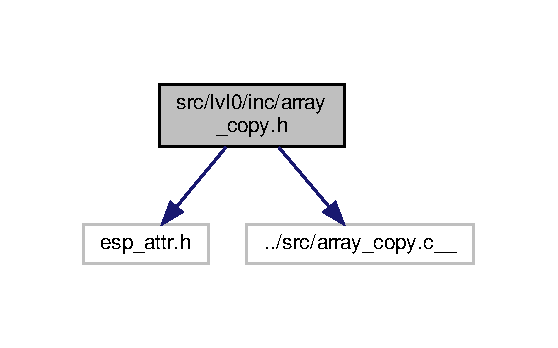
\includegraphics[width=256pt]{array__copy_8h__incl}
\end{center}
\end{figure}
This graph shows which files directly or indirectly include this file\+:
\nopagebreak
\begin{figure}[H]
\begin{center}
\leavevmode
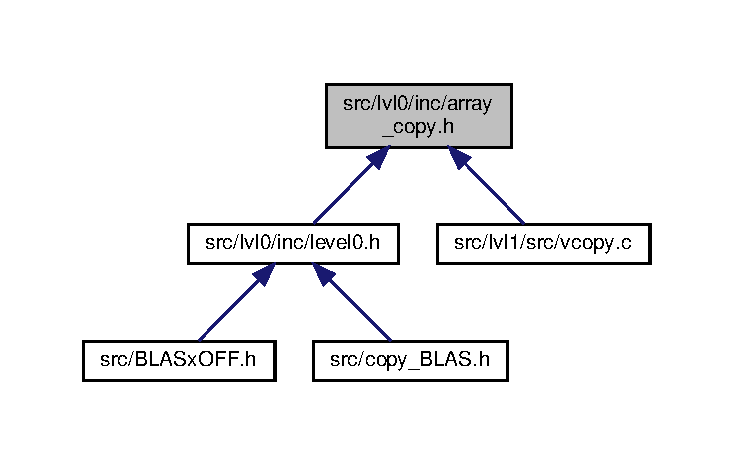
\includegraphics[width=350pt]{array__copy_8h__dep__incl}
\end{center}
\end{figure}
\subsection*{Functions}
\begin{DoxyCompactItemize}
\item 
void I\+R\+A\+M\+\_\+\+A\+T\+TR \hyperlink{array__copy_8h_a6eff457f740569ba50b92c95bd5193b1}{array\+\_\+copy} (float $\ast$arr\+Dst, const float $\ast$arr\+Src, const unsigned int start, const unsigned int end) \+\_\+\+\_\+attribute\+\_\+\+\_\+((always\+\_\+inline)) \+\_\+\+\_\+attribute\+\_\+\+\_\+((nonull))
\end{DoxyCompactItemize}


\subsection{Function Documentation}
\mbox{\Hypertarget{array__copy_8h_a6eff457f740569ba50b92c95bd5193b1}\label{array__copy_8h_a6eff457f740569ba50b92c95bd5193b1}} 
\index{array\+\_\+copy.\+h@{array\+\_\+copy.\+h}!array\+\_\+copy@{array\+\_\+copy}}
\index{array\+\_\+copy@{array\+\_\+copy}!array\+\_\+copy.\+h@{array\+\_\+copy.\+h}}
\subsubsection{\texorpdfstring{array\+\_\+copy()}{array\_copy()}}
{\footnotesize\ttfamily void I\+R\+A\+M\+\_\+\+A\+T\+TR array\+\_\+copy (\begin{DoxyParamCaption}\item[{float $\ast$}]{arr\+Dst,  }\item[{const float $\ast$}]{arr\+Src,  }\item[{const unsigned int}]{start,  }\item[{const unsigned int}]{end }\end{DoxyParamCaption})}

This function copies the elements of one arrays into another array 
\begin{DoxyParams}{Parameters}
{\em arr\+Dst} & Array pointer destination to copy source data into \\
\hline
{\em arr\+Src} & Array pointer for source data \\
\hline
{\em start} & Starting element index to loop across \\
\hline
{\em end} & Last element index to loop across \\
\hline
\end{DoxyParams}
Here is the caller graph for this function\+:
\nopagebreak
\begin{figure}[H]
\begin{center}
\leavevmode
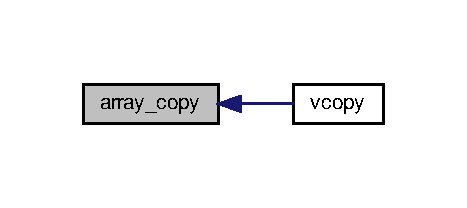
\includegraphics[width=224pt]{array__copy_8h_a6eff457f740569ba50b92c95bd5193b1_icgraph}
\end{center}
\end{figure}

\hypertarget{array__dot_8h}{}\section{src/lvl0/inc/array\+\_\+dot.h File Reference}
\label{array__dot_8h}\index{src/lvl0/inc/array\+\_\+dot.\+h@{src/lvl0/inc/array\+\_\+dot.\+h}}
{\ttfamily \#include \char`\"{}esp\+\_\+attr.\+h\char`\"{}}\newline
{\ttfamily \#include \char`\"{}../src/array\+\_\+dot.\+c\+\_\+\+\_\+\char`\"{}}\newline
Include dependency graph for array\+\_\+dot.\+h\+:
\nopagebreak
\begin{figure}[H]
\begin{center}
\leavevmode
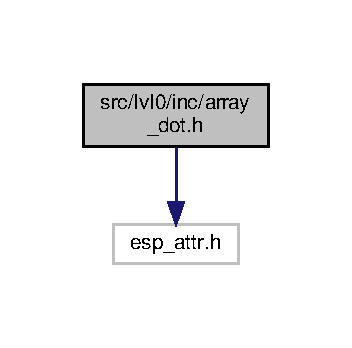
\includegraphics[width=260pt]{array__dot_8h__incl}
\end{center}
\end{figure}
This graph shows which files directly or indirectly include this file\+:
\nopagebreak
\begin{figure}[H]
\begin{center}
\leavevmode
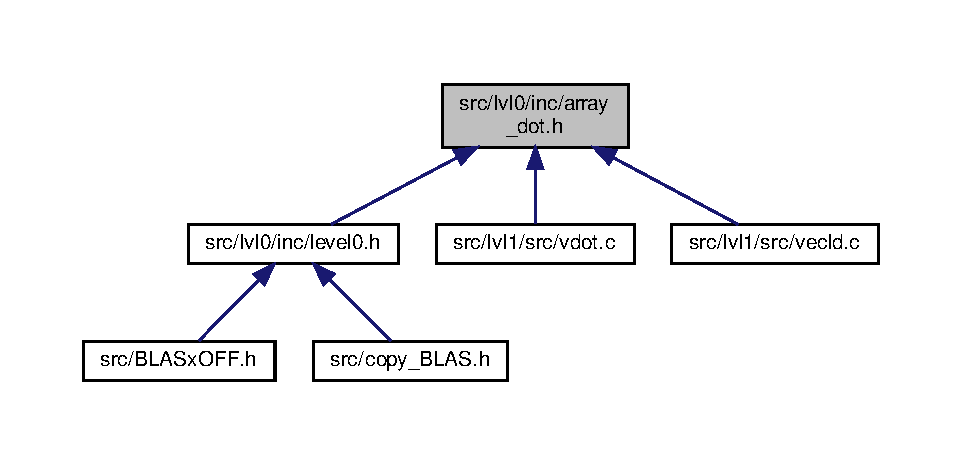
\includegraphics[width=345pt]{array__dot_8h__dep__incl}
\end{center}
\end{figure}
\subsection*{Functions}
\begin{DoxyCompactItemize}
\item 
void I\+R\+A\+M\+\_\+\+A\+T\+TR \hyperlink{array__dot_8h_a5f226f010b6fa6dc2111595f46e623b0}{array\+\_\+dot} (float $\ast$scl\+Res, const float $\ast$arr\+OprA, const float $\ast$arr\+OprB, const unsigned int start, const unsigned int end) \+\_\+\+\_\+attribute\+\_\+\+\_\+((always\+\_\+inline)) \+\_\+\+\_\+attribute\+\_\+\+\_\+((nonull))
\end{DoxyCompactItemize}


\subsection{Function Documentation}
\mbox{\Hypertarget{array__dot_8h_a5f226f010b6fa6dc2111595f46e623b0}\label{array__dot_8h_a5f226f010b6fa6dc2111595f46e623b0}} 
\index{array\+\_\+dot.\+h@{array\+\_\+dot.\+h}!array\+\_\+dot@{array\+\_\+dot}}
\index{array\+\_\+dot@{array\+\_\+dot}!array\+\_\+dot.\+h@{array\+\_\+dot.\+h}}
\subsubsection{\texorpdfstring{array\+\_\+dot()}{array\_dot()}}
{\footnotesize\ttfamily void I\+R\+A\+M\+\_\+\+A\+T\+TR array\+\_\+dot (\begin{DoxyParamCaption}\item[{float $\ast$}]{scl\+Res,  }\item[{const float $\ast$}]{arr\+OprA,  }\item[{const float $\ast$}]{arr\+OprB,  }\item[{const unsigned int}]{start,  }\item[{const unsigned int}]{end }\end{DoxyParamCaption})}

This function computes the dot product between two arrays 
\begin{DoxyParams}{Parameters}
{\em scl\+Res} & Array pointer where the result will be stored \\
\hline
{\em arr\+OprA} & Array pointer for the 1st operand \\
\hline
{\em arr\+OprB} & Array pointer for the 2nd operand \\
\hline
{\em start} & Starting element index to loop across \\
\hline
{\em end} & Last element index to loop across \\
\hline
\end{DoxyParams}
Here is the caller graph for this function\+:
\nopagebreak
\begin{figure}[H]
\begin{center}
\leavevmode
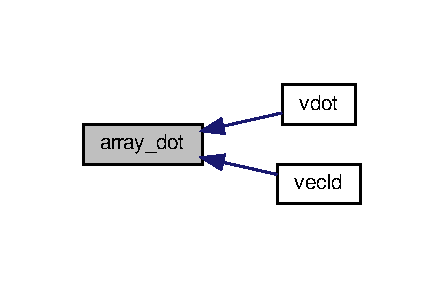
\includegraphics[width=208pt]{array__dot_8h_a5f226f010b6fa6dc2111595f46e623b0_icgraph}
\end{center}
\end{figure}

\hypertarget{array__mscl_8h}{}\section{src/lvl0/inc/array\+\_\+mscl.h File Reference}
\label{array__mscl_8h}\index{src/lvl0/inc/array\+\_\+mscl.\+h@{src/lvl0/inc/array\+\_\+mscl.\+h}}
{\ttfamily \#include \char`\"{}esp\+\_\+attr.\+h\char`\"{}}\newline
{\ttfamily \#include \char`\"{}../src/array\+\_\+mscl.\+c\char`\"{}}\newline
Include dependency graph for array\+\_\+mscl.\+h\+:\nopagebreak
\begin{figure}[H]
\begin{center}
\leavevmode
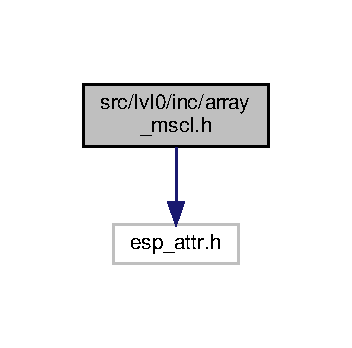
\includegraphics[width=256pt]{array__mscl_8h__incl}
\end{center}
\end{figure}
This graph shows which files directly or indirectly include this file\+:
\nopagebreak
\begin{figure}[H]
\begin{center}
\leavevmode
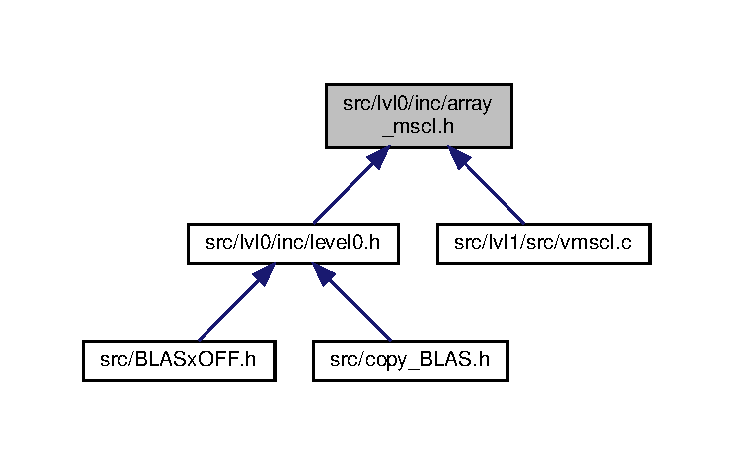
\includegraphics[width=284pt]{array__mscl_8h__dep__incl}
\end{center}
\end{figure}
\subsection*{Functions}
\begin{DoxyCompactItemize}
\item 
void I\+R\+A\+M\+\_\+\+A\+T\+TR \hyperlink{array__mscl_8h_a2fb8bc49731c026d4d80393cb780b8cf}{array\+\_\+mscl} (float $\ast$arr\+Res, const float $\ast$arr\+Opr, const unsigned int start, const unsigned int end, const float scl\+Opr) \+\_\+\+\_\+attribute\+\_\+\+\_\+((always\+\_\+inline)) \+\_\+\+\_\+attribute\+\_\+\+\_\+((nonull))
\end{DoxyCompactItemize}


\subsection{Function Documentation}
\mbox{\Hypertarget{array__mscl_8h_a2fb8bc49731c026d4d80393cb780b8cf}\label{array__mscl_8h_a2fb8bc49731c026d4d80393cb780b8cf}} 
\index{array\+\_\+mscl.\+h@{array\+\_\+mscl.\+h}!array\+\_\+mscl@{array\+\_\+mscl}}
\index{array\+\_\+mscl@{array\+\_\+mscl}!array\+\_\+mscl.\+h@{array\+\_\+mscl.\+h}}
\subsubsection{\texorpdfstring{array\+\_\+mscl()}{array\_mscl()}}
{\footnotesize\ttfamily void I\+R\+A\+M\+\_\+\+A\+T\+TR array\+\_\+mscl (\begin{DoxyParamCaption}\item[{float $\ast$}]{arr\+Res,  }\item[{const float $\ast$}]{arr\+Opr,  }\item[{const unsigned int}]{start,  }\item[{const unsigned int}]{end,  }\item[{const float}]{scl\+Opr }\end{DoxyParamCaption})}

This function multiplies each element of an array by a scalar 
\begin{DoxyParams}{Parameters}
{\em arr\+Res} & Array pointer where the result will be stored \\
\hline
{\em arr\+Opr} & Array pointer for the 1st operand \\
\hline
{\em start} & Starting element index to loop across \\
\hline
{\em end} & Last element index to loop across \\
\hline
{\em scl\+Opr} & float for the 2nd Scalar operand \\
\hline
\end{DoxyParams}

\hypertarget{array__mult_8h}{}\section{src/lvl0/inc/array\+\_\+mult.h File Reference}
\label{array__mult_8h}\index{src/lvl0/inc/array\+\_\+mult.\+h@{src/lvl0/inc/array\+\_\+mult.\+h}}
{\ttfamily \#include \char`\"{}esp\+\_\+attr.\+h\char`\"{}}\newline
Include dependency graph for array\+\_\+mult.\+h\+:
\nopagebreak
\begin{figure}[H]
\begin{center}
\leavevmode
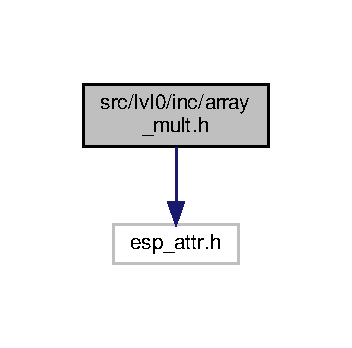
\includegraphics[width=169pt]{array__mult_8h__incl}
\end{center}
\end{figure}
This graph shows which files directly or indirectly include this file\+:
\nopagebreak
\begin{figure}[H]
\begin{center}
\leavevmode
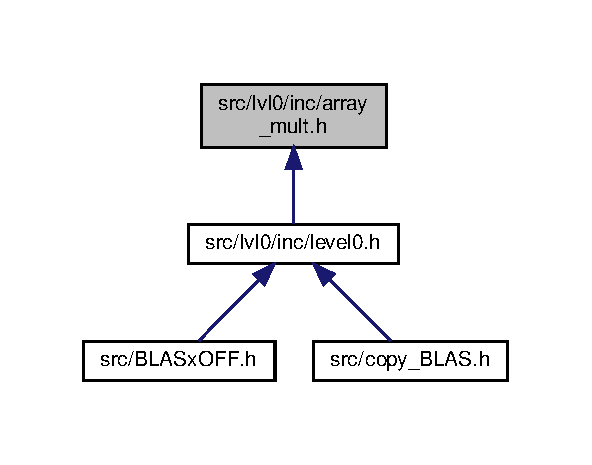
\includegraphics[width=350pt]{array__mult_8h__dep__incl}
\end{center}
\end{figure}
\subsection*{Macros}
\begin{DoxyCompactItemize}
\item 
\#define \hyperlink{array__mult_8h_ae6ff41290217771563cb86884152a2d0}{A\+R\+R\+A\+Y\+\_\+\+M\+U\+L\+T\+\_\+H}
\end{DoxyCompactItemize}
\subsection*{Functions}
\begin{DoxyCompactItemize}
\item 
void I\+R\+A\+M\+\_\+\+A\+T\+TR \hyperlink{array__mult_8h_a734470c4a3d399eca901aa8851286dbc}{\+\_\+\+\_\+attribute\+\_\+\+\_\+} ((always\+\_\+inline)) \+\_\+\+\_\+attribute\+\_\+\+\_\+((nonull)) array\+\_\+mult(float $\ast$arr\+Res
\end{DoxyCompactItemize}
\subsection*{Variables}
\begin{DoxyCompactItemize}
\item 
void I\+R\+A\+M\+\_\+\+A\+T\+TR const float $\ast$ \hyperlink{array__mult_8h_a5e4e071457fdcdd98fd22e75c6bfc555}{arr\+OprA}
\begin{DoxyCompactList}\small\item\em $<$ Array pointer where the result will be stored \end{DoxyCompactList}\item 
void I\+R\+A\+M\+\_\+\+A\+T\+TR const float const float $\ast$ \hyperlink{array__mult_8h_ad0fdcae3b6e2275dc980d15e3726a6a1}{arr\+OprB}
\begin{DoxyCompactList}\small\item\em Array pointer for the 2nd operand. \end{DoxyCompactList}\item 
void I\+R\+A\+M\+\_\+\+A\+T\+TR const float const float const unsigned int \hyperlink{array__mult_8h_a0549b2187026de7f72c6b3214fa437d5}{start}
\begin{DoxyCompactList}\small\item\em Starting element index to loop across. \end{DoxyCompactList}\item 
void I\+R\+A\+M\+\_\+\+A\+T\+TR const float const float const unsigned int const unsigned int \hyperlink{array__mult_8h_a68c28899964e31626b3c9e42853f0d42}{end}
\begin{DoxyCompactList}\small\item\em $<$ Last element index to loop across \end{DoxyCompactList}\end{DoxyCompactItemize}


\subsection{Macro Definition Documentation}
\mbox{\Hypertarget{array__mult_8h_ae6ff41290217771563cb86884152a2d0}\label{array__mult_8h_ae6ff41290217771563cb86884152a2d0}} 
\index{array\+\_\+mult.\+h@{array\+\_\+mult.\+h}!A\+R\+R\+A\+Y\+\_\+\+M\+U\+L\+T\+\_\+H@{A\+R\+R\+A\+Y\+\_\+\+M\+U\+L\+T\+\_\+H}}
\index{A\+R\+R\+A\+Y\+\_\+\+M\+U\+L\+T\+\_\+H@{A\+R\+R\+A\+Y\+\_\+\+M\+U\+L\+T\+\_\+H}!array\+\_\+mult.\+h@{array\+\_\+mult.\+h}}
\subsubsection{\texorpdfstring{A\+R\+R\+A\+Y\+\_\+\+M\+U\+L\+T\+\_\+H}{ARRAY\_MULT\_H}}
{\footnotesize\ttfamily \#define A\+R\+R\+A\+Y\+\_\+\+M\+U\+L\+T\+\_\+H}

This function multiplies elements of an array by a scalar 

\subsection{Function Documentation}
\mbox{\Hypertarget{array__mult_8h_a734470c4a3d399eca901aa8851286dbc}\label{array__mult_8h_a734470c4a3d399eca901aa8851286dbc}} 
\index{array\+\_\+mult.\+h@{array\+\_\+mult.\+h}!\+\_\+\+\_\+attribute\+\_\+\+\_\+@{\+\_\+\+\_\+attribute\+\_\+\+\_\+}}
\index{\+\_\+\+\_\+attribute\+\_\+\+\_\+@{\+\_\+\+\_\+attribute\+\_\+\+\_\+}!array\+\_\+mult.\+h@{array\+\_\+mult.\+h}}
\subsubsection{\texorpdfstring{\+\_\+\+\_\+attribute\+\_\+\+\_\+()}{\_\_attribute\_\_()}}
{\footnotesize\ttfamily void I\+R\+A\+M\+\_\+\+A\+T\+TR \+\_\+\+\_\+attribute\+\_\+\+\_\+ (\begin{DoxyParamCaption}\item[{(always\+\_\+inline)}]{ }\end{DoxyParamCaption})}



\subsection{Variable Documentation}
\mbox{\Hypertarget{array__mult_8h_a5e4e071457fdcdd98fd22e75c6bfc555}\label{array__mult_8h_a5e4e071457fdcdd98fd22e75c6bfc555}} 
\index{array\+\_\+mult.\+h@{array\+\_\+mult.\+h}!arr\+OprA@{arr\+OprA}}
\index{arr\+OprA@{arr\+OprA}!array\+\_\+mult.\+h@{array\+\_\+mult.\+h}}
\subsubsection{\texorpdfstring{arr\+OprA}{arrOprA}}
{\footnotesize\ttfamily void I\+R\+A\+M\+\_\+\+A\+T\+TR const float$\ast$ arr\+OprA}



$<$ Array pointer where the result will be stored 

Array pointer for the 1st operand \mbox{\Hypertarget{array__mult_8h_ad0fdcae3b6e2275dc980d15e3726a6a1}\label{array__mult_8h_ad0fdcae3b6e2275dc980d15e3726a6a1}} 
\index{array\+\_\+mult.\+h@{array\+\_\+mult.\+h}!arr\+OprB@{arr\+OprB}}
\index{arr\+OprB@{arr\+OprB}!array\+\_\+mult.\+h@{array\+\_\+mult.\+h}}
\subsubsection{\texorpdfstring{arr\+OprB}{arrOprB}}
{\footnotesize\ttfamily void I\+R\+A\+M\+\_\+\+A\+T\+TR const float const float$\ast$ arr\+OprB}



Array pointer for the 2nd operand. 

\mbox{\Hypertarget{array__mult_8h_a68c28899964e31626b3c9e42853f0d42}\label{array__mult_8h_a68c28899964e31626b3c9e42853f0d42}} 
\index{array\+\_\+mult.\+h@{array\+\_\+mult.\+h}!end@{end}}
\index{end@{end}!array\+\_\+mult.\+h@{array\+\_\+mult.\+h}}
\subsubsection{\texorpdfstring{end}{end}}
{\footnotesize\ttfamily void I\+R\+A\+M\+\_\+\+A\+T\+TR const float const float const unsigned int const unsigned int end}

{\bfseries Initial value\+:}
\begin{DoxyCode}
\{
    \textcolor{keywordflow}{for}(\textcolor{keywordtype}{unsigned} \textcolor{keywordtype}{int} I=\hyperlink{array__mult_8h_a0549b2187026de7f72c6b3214fa437d5}{start}; I<\hyperlink{array__mult_8h_a68c28899964e31626b3c9e42853f0d42}{end}; ++I) \{
      arrRes[I] = \hyperlink{array__mult_8h_a5e4e071457fdcdd98fd22e75c6bfc555}{arrOprA}[I] * \hyperlink{array__mult_8h_ad0fdcae3b6e2275dc980d15e3726a6a1}{arrOprB}[I];
    \}
    \textcolor{keywordflow}{return}
\end{DoxyCode}


$<$ Last element index to loop across 

\mbox{\Hypertarget{array__mult_8h_a0549b2187026de7f72c6b3214fa437d5}\label{array__mult_8h_a0549b2187026de7f72c6b3214fa437d5}} 
\index{array\+\_\+mult.\+h@{array\+\_\+mult.\+h}!start@{start}}
\index{start@{start}!array\+\_\+mult.\+h@{array\+\_\+mult.\+h}}
\subsubsection{\texorpdfstring{start}{start}}
{\footnotesize\ttfamily void I\+R\+A\+M\+\_\+\+A\+T\+TR const float const float const unsigned int start}



Starting element index to loop across. 


\hypertarget{array__print_8h}{}\section{src/lvl0/inc/array\+\_\+print.h File Reference}
\label{array__print_8h}\index{src/lvl0/inc/array\+\_\+print.\+h@{src/lvl0/inc/array\+\_\+print.\+h}}
{\ttfamily \#include $<$stdio.\+h$>$}\newline
{\ttfamily \#include \char`\"{}esp\+\_\+attr.\+h\char`\"{}}\newline
{\ttfamily \#include \char`\"{}../src/array\+\_\+print.\+c\char`\"{}}\newline
Include dependency graph for array\+\_\+print.\+h\+:\nopagebreak
\begin{figure}[H]
\begin{center}
\leavevmode
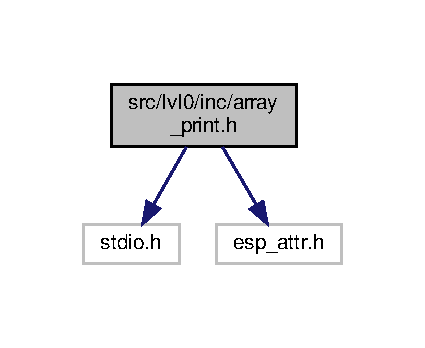
\includegraphics[width=269pt]{array__print_8h__incl}
\end{center}
\end{figure}
This graph shows which files directly or indirectly include this file\+:
\nopagebreak
\begin{figure}[H]
\begin{center}
\leavevmode
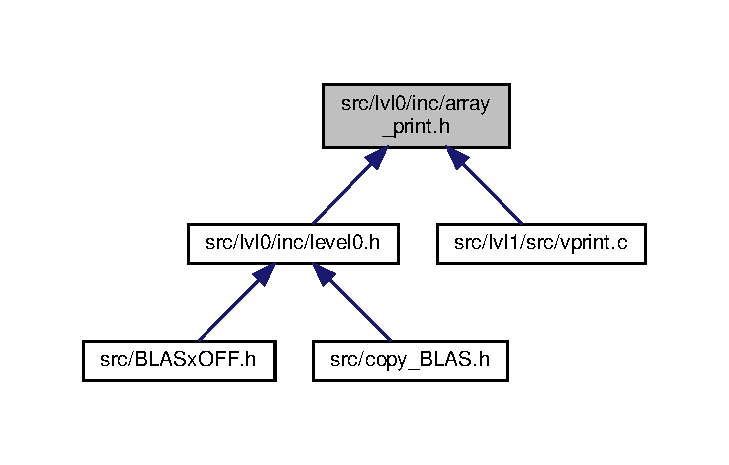
\includegraphics[width=284pt]{array__print_8h__dep__incl}
\end{center}
\end{figure}
\subsection*{Functions}
\begin{DoxyCompactItemize}
\item 
void I\+R\+A\+M\+\_\+\+A\+T\+TR \hyperlink{array__print_8h_a1452525829b0cf910e14b65121a0c53d}{array\+\_\+print} (char $\ast$string, const float $\ast$arr\+Src, const unsigned int start, const unsigned int end) \+\_\+\+\_\+attribute\+\_\+\+\_\+((always\+\_\+inline)) \+\_\+\+\_\+attribute\+\_\+\+\_\+((nonull))
\end{DoxyCompactItemize}


\subsection{Function Documentation}
\mbox{\Hypertarget{array__print_8h_a1452525829b0cf910e14b65121a0c53d}\label{array__print_8h_a1452525829b0cf910e14b65121a0c53d}} 
\index{array\+\_\+print.\+h@{array\+\_\+print.\+h}!array\+\_\+print@{array\+\_\+print}}
\index{array\+\_\+print@{array\+\_\+print}!array\+\_\+print.\+h@{array\+\_\+print.\+h}}
\subsubsection{\texorpdfstring{array\+\_\+print()}{array\_print()}}
{\footnotesize\ttfamily void I\+R\+A\+M\+\_\+\+A\+T\+TR array\+\_\+print (\begin{DoxyParamCaption}\item[{char $\ast$}]{string,  }\item[{const float $\ast$}]{arr\+Src,  }\item[{const unsigned int}]{start,  }\item[{const unsigned int}]{end }\end{DoxyParamCaption})}

Returns a pointer to a printable string of the data in a Vector 
\begin{DoxyParams}{Parameters}
{\em string} & Pointer to string buffer for printing \\
\hline
{\em arr\+Src} & Array pointer for source data \\
\hline
{\em start} & Starting element index to loop across \\
\hline
{\em end} & Last element index to loop across \\
\hline
\end{DoxyParams}

\hypertarget{array__puts_8h}{}\section{src/lvl0/inc/array\+\_\+puts.h File Reference}
\label{array__puts_8h}\index{src/lvl0/inc/array\+\_\+puts.\+h@{src/lvl0/inc/array\+\_\+puts.\+h}}
{\ttfamily \#include \char`\"{}esp\+\_\+attr.\+h\char`\"{}}\newline
{\ttfamily \#include \char`\"{}../src/array\+\_\+puts.\+c\char`\"{}}\newline
Include dependency graph for array\+\_\+puts.\+h\+:\nopagebreak
\begin{figure}[H]
\begin{center}
\leavevmode
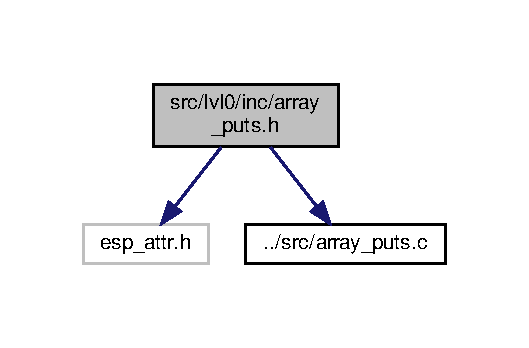
\includegraphics[width=254pt]{array__puts_8h__incl}
\end{center}
\end{figure}
This graph shows which files directly or indirectly include this file\+:
\nopagebreak
\begin{figure}[H]
\begin{center}
\leavevmode
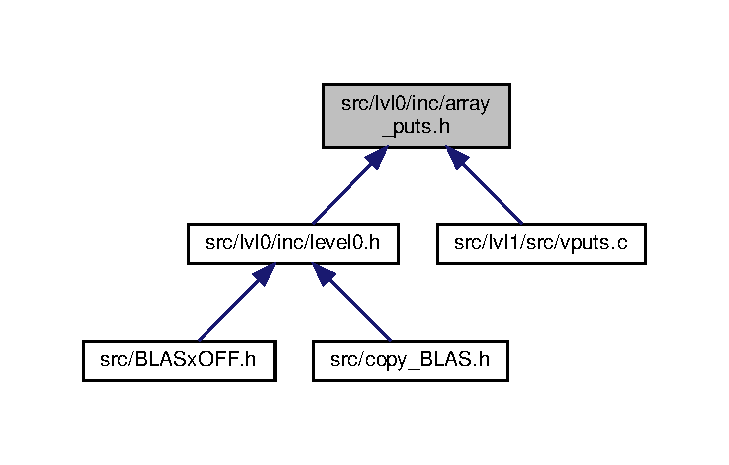
\includegraphics[width=284pt]{array__puts_8h__dep__incl}
\end{center}
\end{figure}
\subsection*{Functions}
\begin{DoxyCompactItemize}
\item 
void I\+R\+A\+M\+\_\+\+A\+T\+TR \hyperlink{array__puts_8h_a173a2544e1e54d9605348701522c160f}{array\+\_\+puts} (char $\ast$string, const float $\ast$arr\+Src, const unsigned int start, const unsigned int end) \+\_\+\+\_\+attribute\+\_\+\+\_\+((always\+\_\+inline)) \+\_\+\+\_\+attribute\+\_\+\+\_\+((nonull))
\end{DoxyCompactItemize}


\subsection{Function Documentation}
\mbox{\Hypertarget{array__puts_8h_a173a2544e1e54d9605348701522c160f}\label{array__puts_8h_a173a2544e1e54d9605348701522c160f}} 
\index{array\+\_\+puts.\+h@{array\+\_\+puts.\+h}!array\+\_\+puts@{array\+\_\+puts}}
\index{array\+\_\+puts@{array\+\_\+puts}!array\+\_\+puts.\+h@{array\+\_\+puts.\+h}}
\subsubsection{\texorpdfstring{array\+\_\+puts()}{array\_puts()}}
{\footnotesize\ttfamily void I\+R\+A\+M\+\_\+\+A\+T\+TR array\+\_\+puts (\begin{DoxyParamCaption}\item[{char $\ast$}]{string,  }\item[{const float $\ast$}]{arr\+Src,  }\item[{const unsigned int}]{start,  }\item[{const unsigned int}]{end }\end{DoxyParamCaption})}

Returns a pointer to a putsable string with the return character \textquotesingle{}~\newline
\textquotesingle{} 
\begin{DoxyParams}{Parameters}
{\em string} & Pointer to string buffer for printing \\
\hline
{\em arr\+Src} & Array pointer for source data \\
\hline
{\em start} & Starting element index to loop across \\
\hline
{\em end} & Last element index to loop across \\
\hline
\end{DoxyParams}

\hypertarget{array__set_8h}{}\section{src/lvl0/inc/array\+\_\+set.h File Reference}
\label{array__set_8h}\index{src/lvl0/inc/array\+\_\+set.\+h@{src/lvl0/inc/array\+\_\+set.\+h}}
{\ttfamily \#include \char`\"{}esp\+\_\+attr.\+h\char`\"{}}\newline
Include dependency graph for array\+\_\+set.\+h\+:
\nopagebreak
\begin{figure}[H]
\begin{center}
\leavevmode
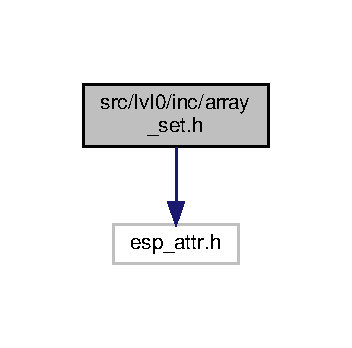
\includegraphics[width=169pt]{array__set_8h__incl}
\end{center}
\end{figure}
This graph shows which files directly or indirectly include this file\+:
\nopagebreak
\begin{figure}[H]
\begin{center}
\leavevmode
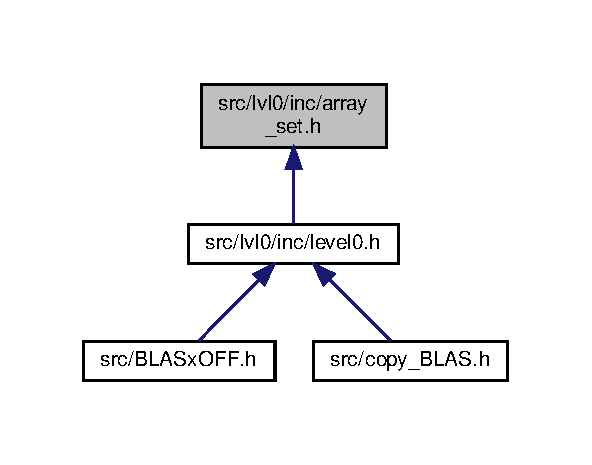
\includegraphics[width=284pt]{array__set_8h__dep__incl}
\end{center}
\end{figure}
\subsection*{Functions}
\begin{DoxyCompactItemize}
\item 
void I\+R\+A\+M\+\_\+\+A\+T\+TR \hyperlink{array__set_8h_a3f568bfbd4fde500e67a7d1ea14a114f}{\+\_\+\+\_\+attribute\+\_\+\+\_\+} ((always\+\_\+inline)) \+\_\+\+\_\+attribute\+\_\+\+\_\+((nonull))
\item 
\hyperlink{array__set_8h_a4783e2ea7e94e79636384acc4c542684}{array\+\_\+set} (float $\ast$arr\+Dst, const float \hyperlink{array__print_8h_a476893ee338bd7d79f15687de2dd39b2}{scl\+Src}, const unsigned int \hyperlink{array__zero_8h_a1951879481f1ba4287d30b0a485429fc}{start}, const unsigned int \hyperlink{array__zero_8h_ae062d39ef5523e038e43c08fa9fe07b4}{end})
\end{DoxyCompactItemize}


\subsection{Function Documentation}
\mbox{\Hypertarget{array__set_8h_a3f568bfbd4fde500e67a7d1ea14a114f}\label{array__set_8h_a3f568bfbd4fde500e67a7d1ea14a114f}} 
\index{array\+\_\+set.\+h@{array\+\_\+set.\+h}!\+\_\+\+\_\+attribute\+\_\+\+\_\+@{\+\_\+\+\_\+attribute\+\_\+\+\_\+}}
\index{\+\_\+\+\_\+attribute\+\_\+\+\_\+@{\+\_\+\+\_\+attribute\+\_\+\+\_\+}!array\+\_\+set.\+h@{array\+\_\+set.\+h}}
\subsubsection{\texorpdfstring{\+\_\+\+\_\+attribute\+\_\+\+\_\+()}{\_\_attribute\_\_()}}
{\footnotesize\ttfamily void I\+R\+A\+M\+\_\+\+A\+T\+TR \+\_\+\+\_\+attribute\+\_\+\+\_\+ (\begin{DoxyParamCaption}\item[{(always\+\_\+inline)}]{ }\end{DoxyParamCaption})\hspace{0.3cm}{\ttfamily [inline]}}

This function set two arrays together element by element

This function add two arrays together element by element

This function adds a scalar too each element in an array


\begin{DoxyItemize}
\item This function is deliberatly placed in Instruction R\+AM. Meaning that this function will always remained cached.
\item the {\bfseries attribute}((always\+\_\+inline)) tells the compiler to A\+L\+W\+A\+YS inline to function reguardless of optimization levels
\item the {\bfseries attribute}((nonull)) tells the compiler that the function\textquotesingle{}s pointer arguments cannot bell N\+U\+LL
\end{DoxyItemize}

This function adds all the elements in an array and returns the sum

This function copies the elements of one arrays into another array

This function computes the dot product between two arrays

This function multiplies each element of an array by a scalar

This function multiplies elements of an array by a scalar

This function Zeros the elements in an array \mbox{\Hypertarget{array__set_8h_a4783e2ea7e94e79636384acc4c542684}\label{array__set_8h_a4783e2ea7e94e79636384acc4c542684}} 
\index{array\+\_\+set.\+h@{array\+\_\+set.\+h}!array\+\_\+set@{array\+\_\+set}}
\index{array\+\_\+set@{array\+\_\+set}!array\+\_\+set.\+h@{array\+\_\+set.\+h}}
\subsubsection{\texorpdfstring{array\+\_\+set()}{array\_set()}}
{\footnotesize\ttfamily array\+\_\+set (\begin{DoxyParamCaption}\item[{float $\ast$}]{arr\+Dst,  }\item[{const float}]{scl\+Src,  }\item[{const unsigned int}]{start,  }\item[{const unsigned int}]{end }\end{DoxyParamCaption})}


\begin{DoxyParams}{Parameters}
{\em arr\+Dst} & Array pointer where the result will be stored \\
\hline
{\em scl\+Src} & Float for the source scalar \\
\hline
{\em start} & Starting element index to loop across \\
\hline
{\em end} & Last element index to loop across \\
\hline
\end{DoxyParams}

\hypertarget{array__subtract_8h}{}\section{src/lvl0/inc/array\+\_\+subtract.h File Reference}
\label{array__subtract_8h}\index{src/lvl0/inc/array\+\_\+subtract.\+h@{src/lvl0/inc/array\+\_\+subtract.\+h}}
{\ttfamily \#include \char`\"{}esp\+\_\+attr.\+h\char`\"{}}\newline
Include dependency graph for array\+\_\+subtract.\+h\+:
\nopagebreak
\begin{figure}[H]
\begin{center}
\leavevmode
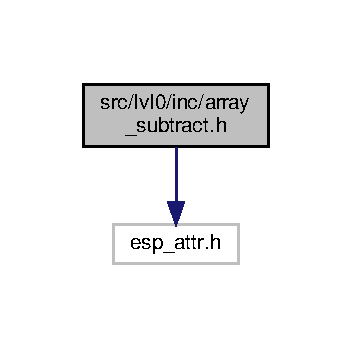
\includegraphics[width=169pt]{array__subtract_8h__incl}
\end{center}
\end{figure}
This graph shows which files directly or indirectly include this file\+:
\nopagebreak
\begin{figure}[H]
\begin{center}
\leavevmode
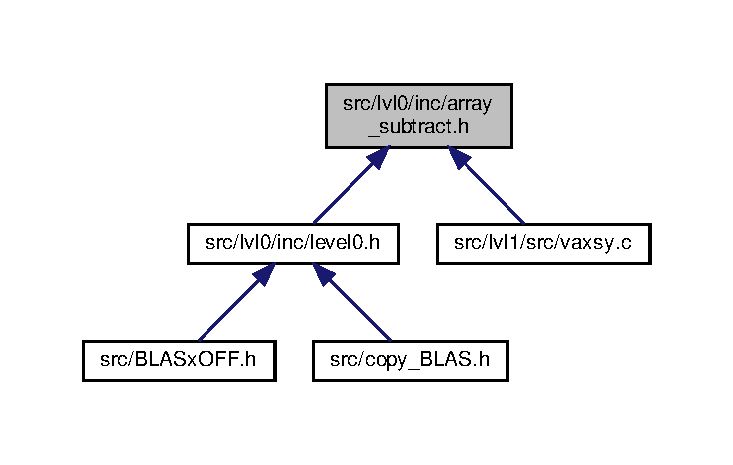
\includegraphics[width=350pt]{array__subtract_8h__dep__incl}
\end{center}
\end{figure}
\subsection*{Functions}
\begin{DoxyCompactItemize}
\item 
void I\+R\+A\+M\+\_\+\+A\+T\+TR \hyperlink{array__subtract_8h_a33d9ae6a3856a1da4409e370ff6f24f8}{\+\_\+\+\_\+attribute\+\_\+\+\_\+} ((always\+\_\+inline)) \+\_\+\+\_\+attribute\+\_\+\+\_\+((nonull)) array\+\_\+substract(float $\ast$arr\+Res
\end{DoxyCompactItemize}
\subsection*{Variables}
\begin{DoxyCompactItemize}
\item 
void I\+R\+A\+M\+\_\+\+A\+T\+TR const float $\ast$ \hyperlink{array__subtract_8h_a5e4e071457fdcdd98fd22e75c6bfc555}{arr\+OprA}
\begin{DoxyCompactList}\small\item\em $<$ Array pointer where the result will be stored \end{DoxyCompactList}\item 
void I\+R\+A\+M\+\_\+\+A\+T\+TR const float const float $\ast$ \hyperlink{array__subtract_8h_ad0fdcae3b6e2275dc980d15e3726a6a1}{arr\+OprB}
\begin{DoxyCompactList}\small\item\em Array pointer for the 2nd operand. \end{DoxyCompactList}\item 
void I\+R\+A\+M\+\_\+\+A\+T\+TR const float const float const unsigned int \hyperlink{array__subtract_8h_a0549b2187026de7f72c6b3214fa437d5}{start}
\begin{DoxyCompactList}\small\item\em Starting element index to loop across. \end{DoxyCompactList}\item 
void I\+R\+A\+M\+\_\+\+A\+T\+TR const float const float const unsigned int const unsigned int \hyperlink{array__subtract_8h_a68c28899964e31626b3c9e42853f0d42}{end}
\begin{DoxyCompactList}\small\item\em $<$ Last element index to loop across \end{DoxyCompactList}\end{DoxyCompactItemize}


\subsection{Function Documentation}
\mbox{\Hypertarget{array__subtract_8h_a33d9ae6a3856a1da4409e370ff6f24f8}\label{array__subtract_8h_a33d9ae6a3856a1da4409e370ff6f24f8}} 
\index{array\+\_\+subtract.\+h@{array\+\_\+subtract.\+h}!\+\_\+\+\_\+attribute\+\_\+\+\_\+@{\+\_\+\+\_\+attribute\+\_\+\+\_\+}}
\index{\+\_\+\+\_\+attribute\+\_\+\+\_\+@{\+\_\+\+\_\+attribute\+\_\+\+\_\+}!array\+\_\+subtract.\+h@{array\+\_\+subtract.\+h}}
\subsubsection{\texorpdfstring{\+\_\+\+\_\+attribute\+\_\+\+\_\+()}{\_\_attribute\_\_()}}
{\footnotesize\ttfamily void I\+R\+A\+M\+\_\+\+A\+T\+TR \+\_\+\+\_\+attribute\+\_\+\+\_\+ (\begin{DoxyParamCaption}\item[{(always\+\_\+inline)}]{ }\end{DoxyParamCaption})}

This function substract two arrays together element by element 

\subsection{Variable Documentation}
\mbox{\Hypertarget{array__subtract_8h_a5e4e071457fdcdd98fd22e75c6bfc555}\label{array__subtract_8h_a5e4e071457fdcdd98fd22e75c6bfc555}} 
\index{array\+\_\+subtract.\+h@{array\+\_\+subtract.\+h}!arr\+OprA@{arr\+OprA}}
\index{arr\+OprA@{arr\+OprA}!array\+\_\+subtract.\+h@{array\+\_\+subtract.\+h}}
\subsubsection{\texorpdfstring{arr\+OprA}{arrOprA}}
{\footnotesize\ttfamily void I\+R\+A\+M\+\_\+\+A\+T\+TR const float$\ast$ arr\+OprA}



$<$ Array pointer where the result will be stored 

Array pointer for the 1st operand \mbox{\Hypertarget{array__subtract_8h_ad0fdcae3b6e2275dc980d15e3726a6a1}\label{array__subtract_8h_ad0fdcae3b6e2275dc980d15e3726a6a1}} 
\index{array\+\_\+subtract.\+h@{array\+\_\+subtract.\+h}!arr\+OprB@{arr\+OprB}}
\index{arr\+OprB@{arr\+OprB}!array\+\_\+subtract.\+h@{array\+\_\+subtract.\+h}}
\subsubsection{\texorpdfstring{arr\+OprB}{arrOprB}}
{\footnotesize\ttfamily void I\+R\+A\+M\+\_\+\+A\+T\+TR const float const float$\ast$ arr\+OprB}



Array pointer for the 2nd operand. 

\mbox{\Hypertarget{array__subtract_8h_a68c28899964e31626b3c9e42853f0d42}\label{array__subtract_8h_a68c28899964e31626b3c9e42853f0d42}} 
\index{array\+\_\+subtract.\+h@{array\+\_\+subtract.\+h}!end@{end}}
\index{end@{end}!array\+\_\+subtract.\+h@{array\+\_\+subtract.\+h}}
\subsubsection{\texorpdfstring{end}{end}}
{\footnotesize\ttfamily void I\+R\+A\+M\+\_\+\+A\+T\+TR const float const float const unsigned int const unsigned int end}

{\bfseries Initial value\+:}
\begin{DoxyCode}
\{
    \textcolor{keywordflow}{for}(\textcolor{keywordtype}{unsigned} \textcolor{keywordtype}{int} I=\hyperlink{array__subtract_8h_a0549b2187026de7f72c6b3214fa437d5}{start}; I<\hyperlink{array__subtract_8h_a68c28899964e31626b3c9e42853f0d42}{end}; ++I) \{
      arrRes[I] = \hyperlink{array__subtract_8h_a5e4e071457fdcdd98fd22e75c6bfc555}{arrOprA} - \hyperlink{array__subtract_8h_ad0fdcae3b6e2275dc980d15e3726a6a1}{arrOprB};
    \}
    \textcolor{keywordflow}{return}
\end{DoxyCode}


$<$ Last element index to loop across 

\mbox{\Hypertarget{array__subtract_8h_a0549b2187026de7f72c6b3214fa437d5}\label{array__subtract_8h_a0549b2187026de7f72c6b3214fa437d5}} 
\index{array\+\_\+subtract.\+h@{array\+\_\+subtract.\+h}!start@{start}}
\index{start@{start}!array\+\_\+subtract.\+h@{array\+\_\+subtract.\+h}}
\subsubsection{\texorpdfstring{start}{start}}
{\footnotesize\ttfamily void I\+R\+A\+M\+\_\+\+A\+T\+TR const float const float const unsigned int start}



Starting element index to loop across. 


\hypertarget{array__swap_8h}{}\section{src/lvl0/inc/array\+\_\+swap.h File Reference}
\label{array__swap_8h}\index{src/lvl0/inc/array\+\_\+swap.\+h@{src/lvl0/inc/array\+\_\+swap.\+h}}
{\ttfamily \#include \char`\"{}esp\+\_\+attr.\+h\char`\"{}}\newline
Include dependency graph for array\+\_\+swap.\+h\+:
\nopagebreak
\begin{figure}[H]
\begin{center}
\leavevmode
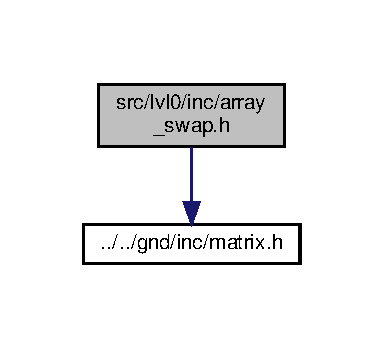
\includegraphics[width=169pt]{array__swap_8h__incl}
\end{center}
\end{figure}
This graph shows which files directly or indirectly include this file\+:\nopagebreak
\begin{figure}[H]
\begin{center}
\leavevmode
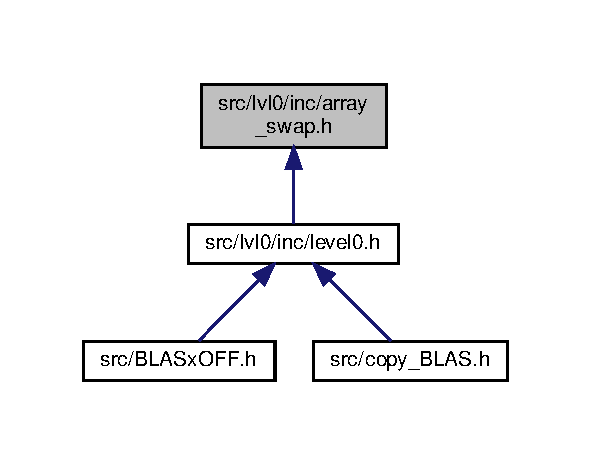
\includegraphics[width=284pt]{array__swap_8h__dep__incl}
\end{center}
\end{figure}
\subsection*{Functions}
\begin{DoxyCompactItemize}
\item 
void I\+R\+A\+M\+\_\+\+A\+T\+TR \hyperlink{array__swap_8h_ac2e028e05235dd050c3da6f604ae22fd}{\+\_\+\+\_\+attribute\+\_\+\+\_\+} ((always\+\_\+inline)) \+\_\+\+\_\+attribute\+\_\+\+\_\+((nonull)) array\+\_\+swap(float $\ast$\hyperlink{array__swap_8h_afbf35f33b730696364a33663ecc97c06}{arr\+Src\+DstA}
\end{DoxyCompactItemize}
\subsection*{Variables}
\begin{DoxyCompactItemize}
\item 
void I\+R\+A\+M\+\_\+\+A\+T\+TR float $\ast$ \hyperlink{array__swap_8h_a4916c4f9ec623c8a595e3282283c2c4c}{arr\+Src\+DstB}
\item 
\hyperlink{array__swap_8h_afbf35f33b730696364a33663ecc97c06}{arr\+Src\+DstA} = \hyperlink{array__swap_8h_a4916c4f9ec623c8a595e3282283c2c4c}{arr\+Src\+DstB}
\item 
\hyperlink{array__swap_8h_a9717e7bbecb906637e86cef6da3d83c2}{return}
\end{DoxyCompactItemize}


\subsection{Function Documentation}
\mbox{\Hypertarget{array__swap_8h_ac2e028e05235dd050c3da6f604ae22fd}\label{array__swap_8h_ac2e028e05235dd050c3da6f604ae22fd}} 
\index{array\+\_\+swap.\+h@{array\+\_\+swap.\+h}!\+\_\+\+\_\+attribute\+\_\+\+\_\+@{\+\_\+\+\_\+attribute\+\_\+\+\_\+}}
\index{\+\_\+\+\_\+attribute\+\_\+\+\_\+@{\+\_\+\+\_\+attribute\+\_\+\+\_\+}!array\+\_\+swap.\+h@{array\+\_\+swap.\+h}}
\subsubsection{\texorpdfstring{\+\_\+\+\_\+attribute\+\_\+\+\_\+()}{\_\_attribute\_\_()}}
{\footnotesize\ttfamily void I\+R\+A\+M\+\_\+\+A\+T\+TR \+\_\+\+\_\+attribute\+\_\+\+\_\+ (\begin{DoxyParamCaption}\item[{(always\+\_\+inline)}]{ }\end{DoxyParamCaption})}

This function swap two arrays together element by element 

\subsection{Variable Documentation}
\mbox{\Hypertarget{array__swap_8h_afbf35f33b730696364a33663ecc97c06}\label{array__swap_8h_afbf35f33b730696364a33663ecc97c06}} 
\index{array\+\_\+swap.\+h@{array\+\_\+swap.\+h}!arr\+Src\+DstA@{arr\+Src\+DstA}}
\index{arr\+Src\+DstA@{arr\+Src\+DstA}!array\+\_\+swap.\+h@{array\+\_\+swap.\+h}}
\subsubsection{\texorpdfstring{arr\+Src\+DstA}{arrSrcDstA}}
{\footnotesize\ttfamily arr\+Src\+DstA = \hyperlink{array__swap_8h_a4916c4f9ec623c8a595e3282283c2c4c}{arr\+Src\+DstB}}

\mbox{\Hypertarget{array__swap_8h_a4916c4f9ec623c8a595e3282283c2c4c}\label{array__swap_8h_a4916c4f9ec623c8a595e3282283c2c4c}} 
\index{array\+\_\+swap.\+h@{array\+\_\+swap.\+h}!arr\+Src\+DstB@{arr\+Src\+DstB}}
\index{arr\+Src\+DstB@{arr\+Src\+DstB}!array\+\_\+swap.\+h@{array\+\_\+swap.\+h}}
\subsubsection{\texorpdfstring{arr\+Src\+DstB}{arrSrcDstB}}
{\footnotesize\ttfamily arr\+Src\+DstB}

{\bfseries Initial value\+:}
\begin{DoxyCode}
\{
    \textcolor{keywordtype}{float} * temp = \hyperlink{array__swap_8h_afbf35f33b730696364a33663ecc97c06}{arrSrcDstA}
\end{DoxyCode}
\mbox{\Hypertarget{array__swap_8h_a9717e7bbecb906637e86cef6da3d83c2}\label{array__swap_8h_a9717e7bbecb906637e86cef6da3d83c2}} 
\index{array\+\_\+swap.\+h@{array\+\_\+swap.\+h}!return@{return}}
\index{return@{return}!array\+\_\+swap.\+h@{array\+\_\+swap.\+h}}
\subsubsection{\texorpdfstring{return}{return}}
{\footnotesize\ttfamily return}


\hypertarget{array__zero_8h}{}\section{src/lvl0/inc/array\+\_\+zero.h File Reference}
\label{array__zero_8h}\index{src/lvl0/inc/array\+\_\+zero.\+h@{src/lvl0/inc/array\+\_\+zero.\+h}}
{\ttfamily \#include \char`\"{}esp\+\_\+attr.\+h\char`\"{}}\newline
{\ttfamily \#include \char`\"{}../src/array\+\_\+zero.\+c\+\_\+\+\_\+\char`\"{}}\newline
Include dependency graph for array\+\_\+zero.\+h\+:
\nopagebreak
\begin{figure}[H]
\begin{center}
\leavevmode
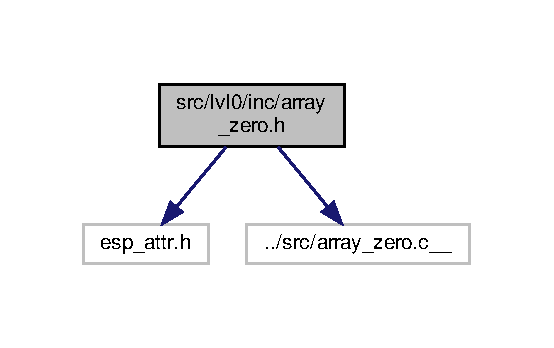
\includegraphics[width=266pt]{array__zero_8h__incl}
\end{center}
\end{figure}
This graph shows which files directly or indirectly include this file\+:\nopagebreak
\begin{figure}[H]
\begin{center}
\leavevmode
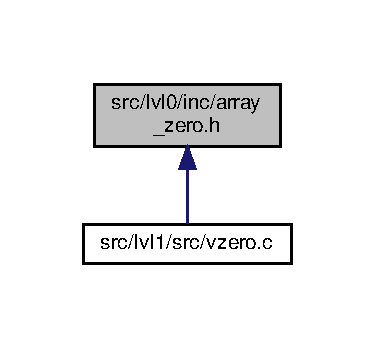
\includegraphics[width=180pt]{array__zero_8h__dep__incl}
\end{center}
\end{figure}
\subsection*{Functions}
\begin{DoxyCompactItemize}
\item 
void I\+R\+A\+M\+\_\+\+A\+T\+TR \hyperlink{array__zero_8h_a56e0537cf29dc30e0320a18e290caa5b}{array\+\_\+zero} (float $\ast$arr\+Dst, const unsigned int start, const unsigned int end) \+\_\+\+\_\+attribute\+\_\+\+\_\+((always\+\_\+inline)) \+\_\+\+\_\+attribute\+\_\+\+\_\+((nonull))
\end{DoxyCompactItemize}


\subsection{Function Documentation}
\mbox{\Hypertarget{array__zero_8h_a56e0537cf29dc30e0320a18e290caa5b}\label{array__zero_8h_a56e0537cf29dc30e0320a18e290caa5b}} 
\index{array\+\_\+zero.\+h@{array\+\_\+zero.\+h}!array\+\_\+zero@{array\+\_\+zero}}
\index{array\+\_\+zero@{array\+\_\+zero}!array\+\_\+zero.\+h@{array\+\_\+zero.\+h}}
\subsubsection{\texorpdfstring{array\+\_\+zero()}{array\_zero()}}
{\footnotesize\ttfamily void I\+R\+A\+M\+\_\+\+A\+T\+TR array\+\_\+zero (\begin{DoxyParamCaption}\item[{float $\ast$}]{arr\+Dst,  }\item[{const unsigned int}]{start,  }\item[{const unsigned int}]{end }\end{DoxyParamCaption})}

This function Zeros the elements in an array 
\begin{DoxyParams}{Parameters}
{\em arr\+Dst} & Array pointer where the result will be stored \\
\hline
{\em start} & Starting element index to loop across \\
\hline
{\em end} & Last element index to loop across \\
\hline
\end{DoxyParams}
Here is the caller graph for this function\+:\nopagebreak
\begin{figure}[H]
\begin{center}
\leavevmode
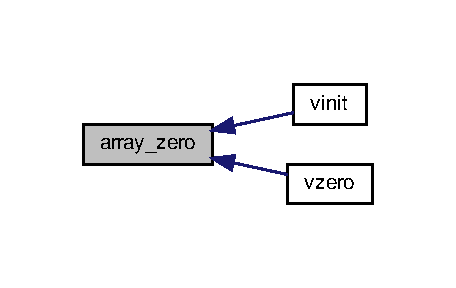
\includegraphics[width=219pt]{array__zero_8h_a56e0537cf29dc30e0320a18e290caa5b_icgraph}
\end{center}
\end{figure}

\hypertarget{level0_8h}{}\section{src/lvl0/inc/level0.h File Reference}
\label{level0_8h}\index{src/lvl0/inc/level0.\+h@{src/lvl0/inc/level0.\+h}}
{\ttfamily \#include \char`\"{}array\+\_\+add.\+h\char`\"{}}\newline
{\ttfamily \#include \char`\"{}array\+\_\+ascl.\+h\char`\"{}}\newline
{\ttfamily \#include \char`\"{}array\+\_\+asum.\+h\char`\"{}}\newline
{\ttfamily \#include \char`\"{}array\+\_\+copy.\+h\char`\"{}}\newline
{\ttfamily \#include \char`\"{}array\+\_\+dot.\+h\char`\"{}}\newline
{\ttfamily \#include \char`\"{}array\+\_\+mscl.\+h\char`\"{}}\newline
{\ttfamily \#include \char`\"{}array\+\_\+mult.\+h\char`\"{}}\newline
{\ttfamily \#include \char`\"{}array\+\_\+print.\+h\char`\"{}}\newline
{\ttfamily \#include \char`\"{}array\+\_\+puts.\+h\char`\"{}}\newline
{\ttfamily \#include \char`\"{}array\+\_\+set.\+h\char`\"{}}\newline
{\ttfamily \#include \char`\"{}array\+\_\+subtract.\+h\char`\"{}}\newline
{\ttfamily \#include \char`\"{}array\+\_\+swap.\+h\char`\"{}}\newline
Include dependency graph for level0.\+h\+:
\nopagebreak
\begin{figure}[H]
\begin{center}
\leavevmode
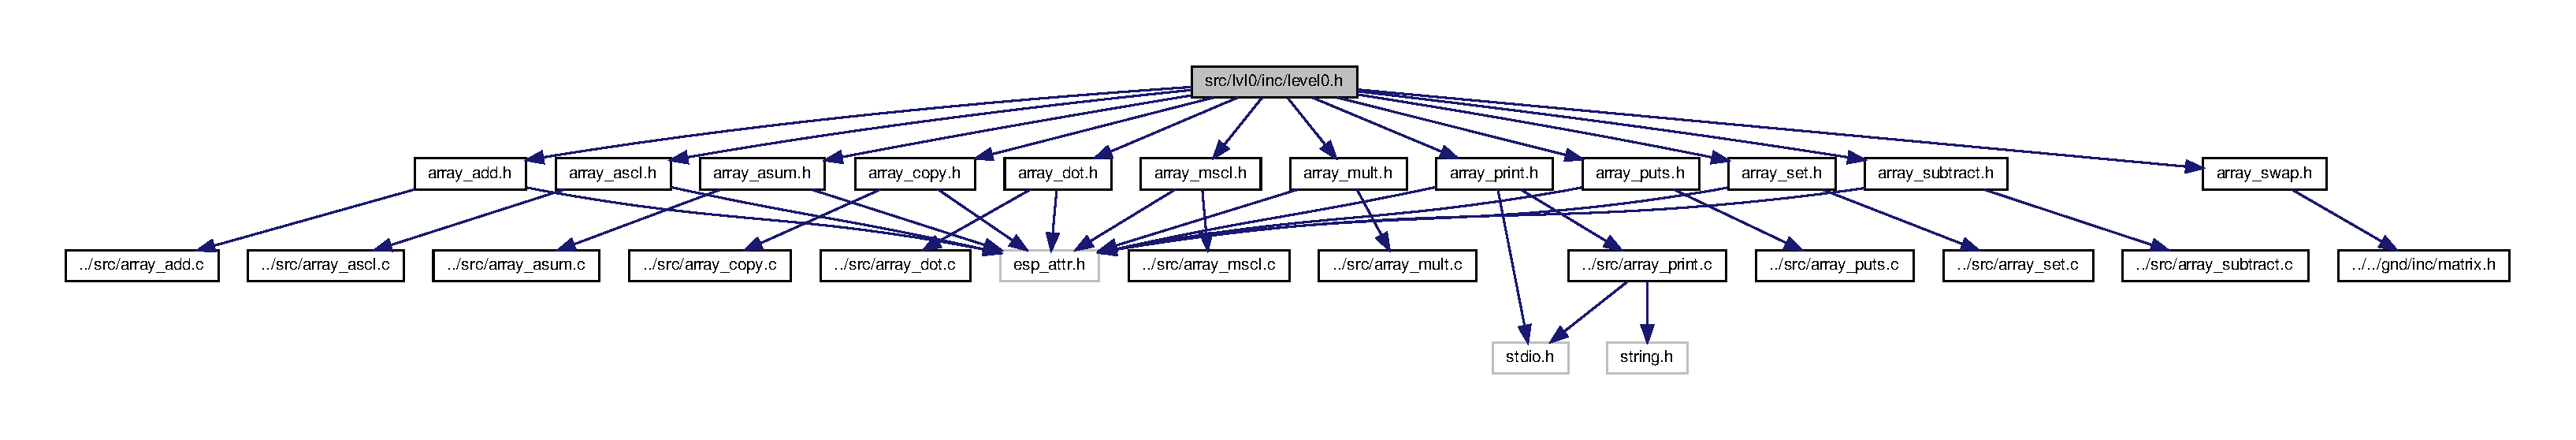
\includegraphics[width=350pt]{level0_8h__incl}
\end{center}
\end{figure}
This graph shows which files directly or indirectly include this file\+:
\nopagebreak
\begin{figure}[H]
\begin{center}
\leavevmode
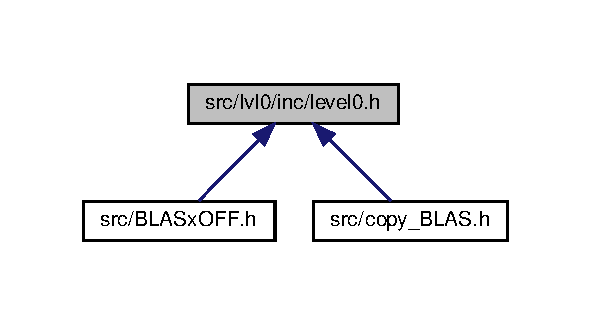
\includegraphics[width=284pt]{level0_8h__dep__incl}
\end{center}
\end{figure}

\hypertarget{level1_8h}{}\section{src/lvl1/inc/level1.h File Reference}
\label{level1_8h}\index{src/lvl1/inc/level1.\+h@{src/lvl1/inc/level1.\+h}}
{\ttfamily \#include \char`\"{}vascl.\+h\char`\"{}}\newline
{\ttfamily \#include \char`\"{}vasum.\+h\char`\"{}}\newline
{\ttfamily \#include \char`\"{}vaxpy.\+h\char`\"{}}\newline
{\ttfamily \#include \char`\"{}vaxsy.\+h\char`\"{}}\newline
{\ttfamily \#include \char`\"{}vcopy.\+h\char`\"{}}\newline
{\ttfamily \#include \char`\"{}vcros.\+h\char`\"{}}\newline
{\ttfamily \#include \char`\"{}vdot.\+h\char`\"{}}\newline
{\ttfamily \#include \char`\"{}vecld.\+h\char`\"{}}\newline
{\ttfamily \#include \char`\"{}vinit.\+h\char`\"{}}\newline
{\ttfamily \#include \char`\"{}vload.\+h\char`\"{}}\newline
{\ttfamily \#include \char`\"{}vmscl.\+h\char`\"{}}\newline
{\ttfamily \#include \char`\"{}vmult.\+h\char`\"{}}\newline
{\ttfamily \#include \char`\"{}vnrm1.\+h\char`\"{}}\newline
{\ttfamily \#include \char`\"{}vnrm2.\+h\char`\"{}}\newline
{\ttfamily \#include \char`\"{}print.\+h\char`\"{}}\newline
{\ttfamily \#include \char`\"{}puts.\+h\char`\"{}}\newline
{\ttfamily \#include \char`\"{}vswap.\+h\char`\"{}}\newline
{\ttfamily \#include \char`\"{}vzero.\+h\char`\"{}}\newline
Include dependency graph for level1.\+h\+:\nopagebreak
\begin{figure}[H]
\begin{center}
\leavevmode
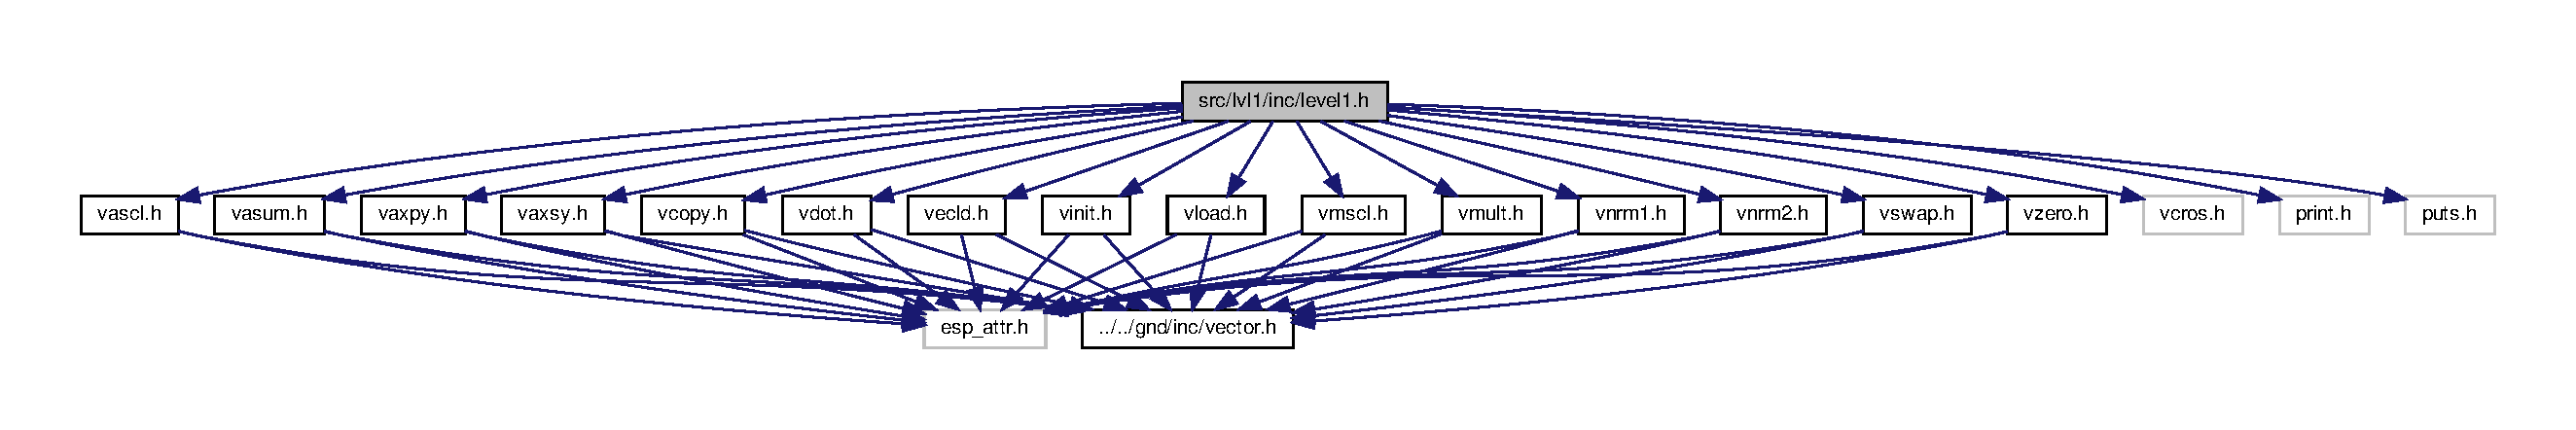
\includegraphics[width=350pt]{level1_8h__incl}
\end{center}
\end{figure}

\hypertarget{vascl_8h}{}\section{src/lvl1/inc/vascl.h File Reference}
\label{vascl_8h}\index{src/lvl1/inc/vascl.\+h@{src/lvl1/inc/vascl.\+h}}
{\ttfamily \#include \char`\"{}esp\+\_\+attr.\+h\char`\"{}}\newline
{\ttfamily \#include \char`\"{}../../gnd/inc/vector.\+h\char`\"{}}\newline
Include dependency graph for vascl.\+h\+:
\nopagebreak
\begin{figure}[H]
\begin{center}
\leavevmode
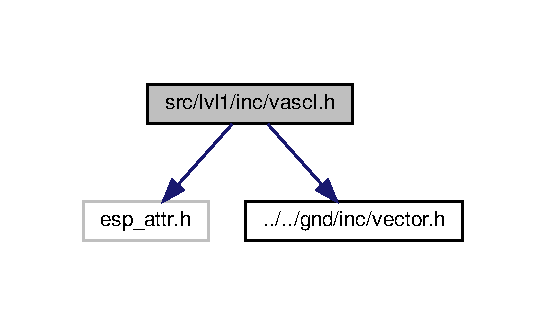
\includegraphics[width=262pt]{vascl_8h__incl}
\end{center}
\end{figure}
This graph shows which files directly or indirectly include this file\+:
\nopagebreak
\begin{figure}[H]
\begin{center}
\leavevmode
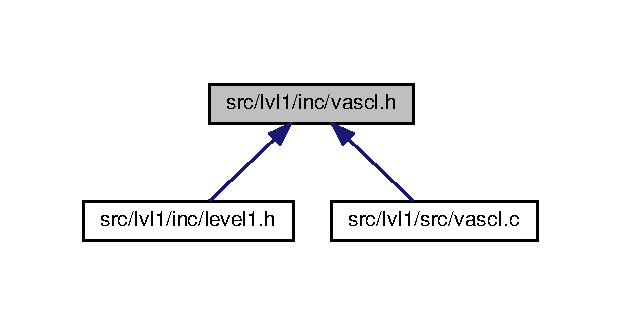
\includegraphics[width=298pt]{vascl_8h__dep__incl}
\end{center}
\end{figure}
\subsection*{Functions}
\begin{DoxyCompactItemize}
\item 
void I\+R\+A\+M\+\_\+\+A\+T\+TR \hyperlink{vascl_8h_aed743cfe105bada98cb98740ad229f52}{vascl} (struct \hyperlink{structvector}{vector} $\ast$v\+Res, const struct \hyperlink{structvector}{vector} $\ast$v\+Opr, const float scl\+Opr) \+\_\+\+\_\+attribute\+\_\+\+\_\+((nonull))
\end{DoxyCompactItemize}


\subsection{Function Documentation}
\mbox{\Hypertarget{vascl_8h_aed743cfe105bada98cb98740ad229f52}\label{vascl_8h_aed743cfe105bada98cb98740ad229f52}} 
\index{vascl.\+h@{vascl.\+h}!vascl@{vascl}}
\index{vascl@{vascl}!vascl.\+h@{vascl.\+h}}
\subsubsection{\texorpdfstring{vascl()}{vascl()}}
{\footnotesize\ttfamily void I\+R\+A\+M\+\_\+\+A\+T\+TR vascl (\begin{DoxyParamCaption}\item[{struct \hyperlink{structvector}{vector} $\ast$}]{v\+Res,  }\item[{const struct \hyperlink{structvector}{vector} $\ast$}]{v\+Opr,  }\item[{const float}]{scl\+Opr }\end{DoxyParamCaption})}

Here is the call graph for this function\+:
\nopagebreak
\begin{figure}[H]
\begin{center}
\leavevmode
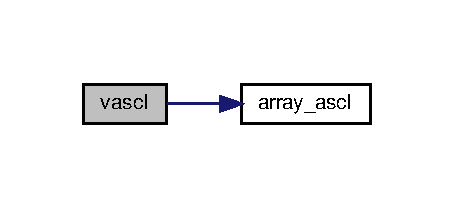
\includegraphics[width=218pt]{vascl_8h_aed743cfe105bada98cb98740ad229f52_cgraph}
\end{center}
\end{figure}

\hypertarget{vasum_8h}{}\section{src/lvl1/inc/vasum.h File Reference}
\label{vasum_8h}\index{src/lvl1/inc/vasum.\+h@{src/lvl1/inc/vasum.\+h}}
{\ttfamily \#include \char`\"{}esp\+\_\+attr.\+h\char`\"{}}\newline
{\ttfamily \#include \char`\"{}../../gnd/inc/vector.\+h\char`\"{}}\newline
Include dependency graph for vasum.\+h\+:\nopagebreak
\begin{figure}[H]
\begin{center}
\leavevmode
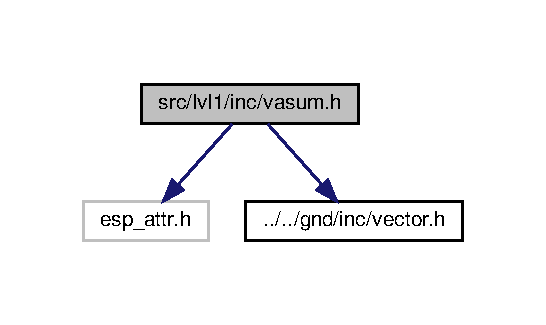
\includegraphics[width=262pt]{vasum_8h__incl}
\end{center}
\end{figure}
This graph shows which files directly or indirectly include this file\+:\nopagebreak
\begin{figure}[H]
\begin{center}
\leavevmode
\includegraphics[width=304pt]{vasum_8h__dep__incl}
\end{center}
\end{figure}
\subsection*{Functions}
\begin{DoxyCompactItemize}
\item 
void I\+R\+A\+M\+\_\+\+A\+T\+TR \hyperlink{vasum_8h_a84cf8d1e138218915d92f209491e5b78}{vasum} (float $\ast$v\+Res, const struct \hyperlink{structvector}{vector} $\ast$v\+Opr) \+\_\+\+\_\+attribute\+\_\+\+\_\+((nonull))
\end{DoxyCompactItemize}


\subsection{Function Documentation}
\mbox{\Hypertarget{vasum_8h_a84cf8d1e138218915d92f209491e5b78}\label{vasum_8h_a84cf8d1e138218915d92f209491e5b78}} 
\index{vasum.\+h@{vasum.\+h}!vasum@{vasum}}
\index{vasum@{vasum}!vasum.\+h@{vasum.\+h}}
\subsubsection{\texorpdfstring{vasum()}{vasum()}}
{\footnotesize\ttfamily void I\+R\+A\+M\+\_\+\+A\+T\+TR vasum (\begin{DoxyParamCaption}\item[{float $\ast$}]{v\+Res,  }\item[{const struct \hyperlink{structvector}{vector} $\ast$}]{v\+Opr }\end{DoxyParamCaption})}

Here is the call graph for this function\+:\nopagebreak
\begin{figure}[H]
\begin{center}
\leavevmode
\includegraphics[width=230pt]{vasum_8h_a84cf8d1e138218915d92f209491e5b78_cgraph}
\end{center}
\end{figure}

\hypertarget{vaxpy_8h}{}\section{src/lvl1/inc/vaxpy.h File Reference}
\label{vaxpy_8h}\index{src/lvl1/inc/vaxpy.\+h@{src/lvl1/inc/vaxpy.\+h}}
{\ttfamily \#include \char`\"{}esp\+\_\+attr.\+h\char`\"{}}\newline
{\ttfamily \#include \char`\"{}../../gnd/inc/vector.\+h\char`\"{}}\newline
Include dependency graph for vaxpy.\+h\+:\nopagebreak
\begin{figure}[H]
\begin{center}
\leavevmode
\includegraphics[width=262pt]{vaxpy_8h__incl}
\end{center}
\end{figure}
This graph shows which files directly or indirectly include this file\+:\nopagebreak
\begin{figure}[H]
\begin{center}
\leavevmode
\includegraphics[width=302pt]{vaxpy_8h__dep__incl}
\end{center}
\end{figure}
\subsection*{Functions}
\begin{DoxyCompactItemize}
\item 
void I\+R\+A\+M\+\_\+\+A\+T\+TR \hyperlink{vaxpy_8h_a389e0b42cc5eb325c6db38677b06e777}{vaxpy} (struct \hyperlink{structvector}{vector} $\ast$v\+Res, const struct \hyperlink{structvector}{vector} $\ast$v\+OprA, const struct \hyperlink{structvector}{vector} $\ast$v\+OprB) \hyperlink{array__zero_8h_a773bfa726d26ed3aba89b686193787aa}{\+\_\+\+\_\+attribute\+\_\+\+\_\+}((nonull))
\end{DoxyCompactItemize}


\subsection{Function Documentation}
\mbox{\Hypertarget{vaxpy_8h_a389e0b42cc5eb325c6db38677b06e777}\label{vaxpy_8h_a389e0b42cc5eb325c6db38677b06e777}} 
\index{vaxpy.\+h@{vaxpy.\+h}!vaxpy@{vaxpy}}
\index{vaxpy@{vaxpy}!vaxpy.\+h@{vaxpy.\+h}}
\subsubsection{\texorpdfstring{vaxpy()}{vaxpy()}}
{\footnotesize\ttfamily void I\+R\+A\+M\+\_\+\+A\+T\+TR vaxpy (\begin{DoxyParamCaption}\item[{struct \hyperlink{structvector}{vector} $\ast$}]{v\+Res,  }\item[{const struct \hyperlink{structvector}{vector} $\ast$}]{v\+OprA,  }\item[{const struct \hyperlink{structvector}{vector} $\ast$}]{v\+OprB }\end{DoxyParamCaption})}


\hypertarget{vaxsy_8h}{}\section{src/lvl1/inc/vaxsy.h File Reference}
\label{vaxsy_8h}\index{src/lvl1/inc/vaxsy.\+h@{src/lvl1/inc/vaxsy.\+h}}
{\ttfamily \#include \char`\"{}esp\+\_\+attr.\+h\char`\"{}}\newline
{\ttfamily \#include \char`\"{}../../gnd/inc/vector.\+h\char`\"{}}\newline
Include dependency graph for vaxsy.\+h\+:
\nopagebreak
\begin{figure}[H]
\begin{center}
\leavevmode
\includegraphics[width=262pt]{vaxsy_8h__incl}
\end{center}
\end{figure}
This graph shows which files directly or indirectly include this file\+:
\nopagebreak
\begin{figure}[H]
\begin{center}
\leavevmode
\includegraphics[width=302pt]{vaxsy_8h__dep__incl}
\end{center}
\end{figure}
\subsection*{Macros}
\begin{DoxyCompactItemize}
\item 
\#define \hyperlink{vaxsy_8h_ad4cdfc81e22ee243365418325295b3f1}{B\+L\+A\+S\+\_\+\+V\+A\+X\+S\+Y\+\_\+H}
\end{DoxyCompactItemize}
\subsection*{Functions}
\begin{DoxyCompactItemize}
\item 
void I\+R\+A\+M\+\_\+\+A\+T\+TR \hyperlink{vaxsy_8h_acffedea41f73b0c3f06eb54a147b3943}{vaxsy} (struct \hyperlink{structvector}{vector} $\ast$v\+Res, const struct \hyperlink{structvector}{vector} $\ast$v\+OprA, const struct \hyperlink{structvector}{vector} $\ast$v\+OprB) \hyperlink{array__zero_8h_a773bfa726d26ed3aba89b686193787aa}{\+\_\+\+\_\+attribute\+\_\+\+\_\+}((nonull))
\end{DoxyCompactItemize}


\subsection{Macro Definition Documentation}
\mbox{\Hypertarget{vaxsy_8h_ad4cdfc81e22ee243365418325295b3f1}\label{vaxsy_8h_ad4cdfc81e22ee243365418325295b3f1}} 
\index{vaxsy.\+h@{vaxsy.\+h}!B\+L\+A\+S\+\_\+\+V\+A\+X\+S\+Y\+\_\+H@{B\+L\+A\+S\+\_\+\+V\+A\+X\+S\+Y\+\_\+H}}
\index{B\+L\+A\+S\+\_\+\+V\+A\+X\+S\+Y\+\_\+H@{B\+L\+A\+S\+\_\+\+V\+A\+X\+S\+Y\+\_\+H}!vaxsy.\+h@{vaxsy.\+h}}
\subsubsection{\texorpdfstring{B\+L\+A\+S\+\_\+\+V\+A\+X\+S\+Y\+\_\+H}{BLAS\_VAXSY\_H}}
{\footnotesize\ttfamily \#define B\+L\+A\+S\+\_\+\+V\+A\+X\+S\+Y\+\_\+H}



\subsection{Function Documentation}
\mbox{\Hypertarget{vaxsy_8h_acffedea41f73b0c3f06eb54a147b3943}\label{vaxsy_8h_acffedea41f73b0c3f06eb54a147b3943}} 
\index{vaxsy.\+h@{vaxsy.\+h}!vaxsy@{vaxsy}}
\index{vaxsy@{vaxsy}!vaxsy.\+h@{vaxsy.\+h}}
\subsubsection{\texorpdfstring{vaxsy()}{vaxsy()}}
{\footnotesize\ttfamily void I\+R\+A\+M\+\_\+\+A\+T\+TR vaxsy (\begin{DoxyParamCaption}\item[{struct \hyperlink{structvector}{vector} $\ast$}]{v\+Res,  }\item[{const struct \hyperlink{structvector}{vector} $\ast$}]{v\+OprA,  }\item[{const struct \hyperlink{structvector}{vector} $\ast$}]{v\+OprB }\end{DoxyParamCaption})}


\hypertarget{vcopy_8h}{}\section{src/lvl1/inc/vcopy.h File Reference}
\label{vcopy_8h}\index{src/lvl1/inc/vcopy.\+h@{src/lvl1/inc/vcopy.\+h}}
{\ttfamily \#include \char`\"{}esp\+\_\+attr.\+h\char`\"{}}\newline
{\ttfamily \#include \char`\"{}../../gnd/inc/vector.\+h\char`\"{}}\newline
Include dependency graph for vcopy.\+h\+:
\nopagebreak
\begin{figure}[H]
\begin{center}
\leavevmode
\includegraphics[width=262pt]{vcopy_8h__incl}
\end{center}
\end{figure}
This graph shows which files directly or indirectly include this file\+:
\nopagebreak
\begin{figure}[H]
\begin{center}
\leavevmode
\includegraphics[width=302pt]{vcopy_8h__dep__incl}
\end{center}
\end{figure}
\subsection*{Functions}
\begin{DoxyCompactItemize}
\item 
void I\+R\+A\+M\+\_\+\+A\+T\+TR \hyperlink{vcopy_8h_aac909f343ab3eb29348b63782d42a21d}{vcopy} (struct \hyperlink{structvector}{vector} $\ast$v\+Dst, const struct \hyperlink{structvector}{vector} $\ast$v\+Src) \+\_\+\+\_\+attribute\+\_\+\+\_\+((nonull))
\end{DoxyCompactItemize}


\subsection{Function Documentation}
\mbox{\Hypertarget{vcopy_8h_aac909f343ab3eb29348b63782d42a21d}\label{vcopy_8h_aac909f343ab3eb29348b63782d42a21d}} 
\index{vcopy.\+h@{vcopy.\+h}!vcopy@{vcopy}}
\index{vcopy@{vcopy}!vcopy.\+h@{vcopy.\+h}}
\subsubsection{\texorpdfstring{vcopy()}{vcopy()}}
{\footnotesize\ttfamily void I\+R\+A\+M\+\_\+\+A\+T\+TR vcopy (\begin{DoxyParamCaption}\item[{struct \hyperlink{structvector}{vector} $\ast$}]{v\+Dst,  }\item[{const struct \hyperlink{structvector}{vector} $\ast$}]{v\+Src }\end{DoxyParamCaption})}

Here is the call graph for this function\+:
\nopagebreak
\begin{figure}[H]
\begin{center}
\leavevmode
\includegraphics[width=224pt]{vcopy_8h_aac909f343ab3eb29348b63782d42a21d_cgraph}
\end{center}
\end{figure}

\hypertarget{vcros3_8h}{}\section{src/lvl1/inc/vcros3.h File Reference}
\label{vcros3_8h}\index{src/lvl1/inc/vcros3.\+h@{src/lvl1/inc/vcros3.\+h}}
{\ttfamily \#include \char`\"{}esp\+\_\+attr.\+h\char`\"{}}\newline
{\ttfamily \#include \char`\"{}../../gnd/inc/vector.\+h\char`\"{}}\newline
Include dependency graph for vcros3.\+h\+:\nopagebreak
\begin{figure}[H]
\begin{center}
\leavevmode
\includegraphics[width=262pt]{vcros3_8h__incl}
\end{center}
\end{figure}
This graph shows which files directly or indirectly include this file\+:\nopagebreak
\begin{figure}[H]
\begin{center}
\leavevmode
\includegraphics[width=185pt]{vcros3_8h__dep__incl}
\end{center}
\end{figure}
\subsection*{Functions}
\begin{DoxyCompactItemize}
\item 
void I\+R\+A\+M\+\_\+\+A\+T\+TR \hyperlink{vcros3_8h_a711e430baa8ecf2cc4f5ce4c584bd1a5}{vcros} (struct \hyperlink{structvector}{vector} $\ast$v\+Res, const struct \hyperlink{structvector}{vector} $\ast$v\+OprA, const struct \hyperlink{structvector}{vector} $\ast$v\+OprB) \hyperlink{array__zero_8h_a773bfa726d26ed3aba89b686193787aa}{\+\_\+\+\_\+attribute\+\_\+\+\_\+}((nonull))
\end{DoxyCompactItemize}


\subsection{Function Documentation}
\mbox{\Hypertarget{vcros3_8h_a711e430baa8ecf2cc4f5ce4c584bd1a5}\label{vcros3_8h_a711e430baa8ecf2cc4f5ce4c584bd1a5}} 
\index{vcros3.\+h@{vcros3.\+h}!vcros@{vcros}}
\index{vcros@{vcros}!vcros3.\+h@{vcros3.\+h}}
\subsubsection{\texorpdfstring{vcros()}{vcros()}}
{\footnotesize\ttfamily void I\+R\+A\+M\+\_\+\+A\+T\+TR vcros (\begin{DoxyParamCaption}\item[{struct \hyperlink{structvector}{vector} $\ast$}]{v\+Res,  }\item[{const struct \hyperlink{structvector}{vector} $\ast$}]{v\+OprA,  }\item[{const struct \hyperlink{structvector}{vector} $\ast$}]{v\+OprB }\end{DoxyParamCaption})}


\hypertarget{vdot_8h}{}\section{src/lvl1/inc/vdot.h File Reference}
\label{vdot_8h}\index{src/lvl1/inc/vdot.\+h@{src/lvl1/inc/vdot.\+h}}
{\ttfamily \#include \char`\"{}esp\+\_\+attr.\+h\char`\"{}}\newline
{\ttfamily \#include \char`\"{}../../gnd/inc/vector.\+h\char`\"{}}\newline
Include dependency graph for vdot.\+h\+:\nopagebreak
\begin{figure}[H]
\begin{center}
\leavevmode
\includegraphics[width=262pt]{vdot_8h__incl}
\end{center}
\end{figure}
This graph shows which files directly or indirectly include this file\+:\nopagebreak
\begin{figure}[H]
\begin{center}
\leavevmode
\includegraphics[width=294pt]{vdot_8h__dep__incl}
\end{center}
\end{figure}
\subsection*{Functions}
\begin{DoxyCompactItemize}
\item 
void I\+R\+A\+M\+\_\+\+A\+T\+TR \hyperlink{vdot_8h_ac792ac8490e9b04f05c2c7ee5073de40}{vdot} (float $\ast$scl\+Res, const struct \hyperlink{structvector}{vector} $\ast$v\+OprA, const struct \hyperlink{structvector}{vector} $\ast$v\+OprB) \+\_\+\+\_\+attribute\+\_\+\+\_\+((nonull))
\end{DoxyCompactItemize}


\subsection{Function Documentation}
\mbox{\Hypertarget{vdot_8h_ac792ac8490e9b04f05c2c7ee5073de40}\label{vdot_8h_ac792ac8490e9b04f05c2c7ee5073de40}} 
\index{vdot.\+h@{vdot.\+h}!vdot@{vdot}}
\index{vdot@{vdot}!vdot.\+h@{vdot.\+h}}
\subsubsection{\texorpdfstring{vdot()}{vdot()}}
{\footnotesize\ttfamily void I\+R\+A\+M\+\_\+\+A\+T\+TR vdot (\begin{DoxyParamCaption}\item[{float $\ast$}]{scl\+Res,  }\item[{const struct \hyperlink{structvector}{vector} $\ast$}]{v\+OprA,  }\item[{const struct \hyperlink{structvector}{vector} $\ast$}]{v\+OprB }\end{DoxyParamCaption})}

Here is the call graph for this function\+:
\nopagebreak
\begin{figure}[H]
\begin{center}
\leavevmode
\includegraphics[width=208pt]{vdot_8h_ac792ac8490e9b04f05c2c7ee5073de40_cgraph}
\end{center}
\end{figure}

\hypertarget{vecld_8h}{}\section{src/lvl1/inc/vecld.h File Reference}
\label{vecld_8h}\index{src/lvl1/inc/vecld.\+h@{src/lvl1/inc/vecld.\+h}}
{\ttfamily \#include \char`\"{}esp\+\_\+attr.\+h\char`\"{}}\newline
{\ttfamily \#include \char`\"{}../../gnd/inc/vector.\+h\char`\"{}}\newline
Include dependency graph for vecld.\+h\+:
\nopagebreak
\begin{figure}[H]
\begin{center}
\leavevmode
\includegraphics[width=262pt]{vecld_8h__incl}
\end{center}
\end{figure}
This graph shows which files directly or indirectly include this file\+:
\nopagebreak
\begin{figure}[H]
\begin{center}
\leavevmode
\includegraphics[width=298pt]{vecld_8h__dep__incl}
\end{center}
\end{figure}
\subsection*{Functions}
\begin{DoxyCompactItemize}
\item 
void I\+R\+A\+M\+\_\+\+A\+T\+TR \hyperlink{vecld_8h_ad6e4b8ff34ecfb5658264fff5003e21f}{vecld} (struct \hyperlink{structvector}{vector} $\ast$v\+Res, const struct \hyperlink{structvector}{vector} $\ast$v\+Opr) \+\_\+\+\_\+attribute\+\_\+\+\_\+((nonull))
\end{DoxyCompactItemize}


\subsection{Function Documentation}
\mbox{\Hypertarget{vecld_8h_ad6e4b8ff34ecfb5658264fff5003e21f}\label{vecld_8h_ad6e4b8ff34ecfb5658264fff5003e21f}} 
\index{vecld.\+h@{vecld.\+h}!vecld@{vecld}}
\index{vecld@{vecld}!vecld.\+h@{vecld.\+h}}
\subsubsection{\texorpdfstring{vecld()}{vecld()}}
{\footnotesize\ttfamily void I\+R\+A\+M\+\_\+\+A\+T\+TR vecld (\begin{DoxyParamCaption}\item[{struct \hyperlink{structvector}{vector} $\ast$}]{v\+Res,  }\item[{const struct \hyperlink{structvector}{vector} $\ast$}]{v\+Opr }\end{DoxyParamCaption})}


\hypertarget{vload_8h}{}\section{src/lvl1/inc/vload.h File Reference}
\label{vload_8h}\index{src/lvl1/inc/vload.\+h@{src/lvl1/inc/vload.\+h}}
{\ttfamily \#include \char`\"{}esp\+\_\+attr.\+h\char`\"{}}\newline
{\ttfamily \#include \char`\"{}../../gnd/inc/vector.\+h\char`\"{}}\newline
Include dependency graph for vload.\+h\+:
\nopagebreak
\begin{figure}[H]
\begin{center}
\leavevmode
\includegraphics[width=262pt]{vload_8h__incl}
\end{center}
\end{figure}
This graph shows which files directly or indirectly include this file\+:
\nopagebreak
\begin{figure}[H]
\begin{center}
\leavevmode
\includegraphics[width=298pt]{vload_8h__dep__incl}
\end{center}
\end{figure}
\subsection*{Macros}
\begin{DoxyCompactItemize}
\item 
\#define \hyperlink{vload_8h_aa6dd057b6c12bb37f6c0e4877acbe62d}{B\+L\+A\+S\+\_\+\+V\+L\+O\+A\+D\+\_\+H}
\end{DoxyCompactItemize}
\subsection*{Functions}
\begin{DoxyCompactItemize}
\item 
void I\+R\+A\+M\+\_\+\+A\+T\+TR \hyperlink{vload_8h_ac2f21f9f48988d56ca820a3c78958237}{vload} (struct \hyperlink{structvector}{vector} $\ast$v\+Dst) \hyperlink{array__zero_8h_a773bfa726d26ed3aba89b686193787aa}{\+\_\+\+\_\+attribute\+\_\+\+\_\+}((nonull))
\end{DoxyCompactItemize}


\subsection{Macro Definition Documentation}
\mbox{\Hypertarget{vload_8h_aa6dd057b6c12bb37f6c0e4877acbe62d}\label{vload_8h_aa6dd057b6c12bb37f6c0e4877acbe62d}} 
\index{vload.\+h@{vload.\+h}!B\+L\+A\+S\+\_\+\+V\+L\+O\+A\+D\+\_\+H@{B\+L\+A\+S\+\_\+\+V\+L\+O\+A\+D\+\_\+H}}
\index{B\+L\+A\+S\+\_\+\+V\+L\+O\+A\+D\+\_\+H@{B\+L\+A\+S\+\_\+\+V\+L\+O\+A\+D\+\_\+H}!vload.\+h@{vload.\+h}}
\subsubsection{\texorpdfstring{B\+L\+A\+S\+\_\+\+V\+L\+O\+A\+D\+\_\+H}{BLAS\_VLOAD\_H}}
{\footnotesize\ttfamily \#define B\+L\+A\+S\+\_\+\+V\+L\+O\+A\+D\+\_\+H}



\subsection{Function Documentation}
\mbox{\Hypertarget{vload_8h_ac2f21f9f48988d56ca820a3c78958237}\label{vload_8h_ac2f21f9f48988d56ca820a3c78958237}} 
\index{vload.\+h@{vload.\+h}!vload@{vload}}
\index{vload@{vload}!vload.\+h@{vload.\+h}}
\subsubsection{\texorpdfstring{vload()}{vload()}}
{\footnotesize\ttfamily void I\+R\+A\+M\+\_\+\+A\+T\+TR vload (\begin{DoxyParamCaption}\item[{struct \hyperlink{structvector}{vector} $\ast$}]{v\+Dst }\end{DoxyParamCaption})}


\hypertarget{vmscl_8h}{}\section{src/lvl1/inc/vmscl.h File Reference}
\label{vmscl_8h}\index{src/lvl1/inc/vmscl.\+h@{src/lvl1/inc/vmscl.\+h}}
{\ttfamily \#include \char`\"{}esp\+\_\+attr.\+h\char`\"{}}\newline
{\ttfamily \#include \char`\"{}../../gnd/inc/vector.\+h\char`\"{}}\newline
Include dependency graph for vmscl.\+h\+:
\nopagebreak
\begin{figure}[H]
\begin{center}
\leavevmode
\includegraphics[width=262pt]{vmscl_8h__incl}
\end{center}
\end{figure}
This graph shows which files directly or indirectly include this file\+:
\nopagebreak
\begin{figure}[H]
\begin{center}
\leavevmode
\includegraphics[width=302pt]{vmscl_8h__dep__incl}
\end{center}
\end{figure}
\subsection*{Functions}
\begin{DoxyCompactItemize}
\item 
void I\+R\+A\+M\+\_\+\+A\+T\+TR \hyperlink{vmscl_8h_a793e14fe55b094d2083af726c9586372}{vmscl} (struct \hyperlink{structvector}{vector} $\ast$v\+Res, const struct \hyperlink{structvector}{vector} $\ast$v\+Opr, const float \hyperlink{array__mscl_8h_a8beac99f3a0446385106d145d3de1f90}{scl\+Opr}) \hyperlink{array__zero_8h_a773bfa726d26ed3aba89b686193787aa}{\+\_\+\+\_\+attribute\+\_\+\+\_\+}((nonull))
\end{DoxyCompactItemize}


\subsection{Function Documentation}
\mbox{\Hypertarget{vmscl_8h_a793e14fe55b094d2083af726c9586372}\label{vmscl_8h_a793e14fe55b094d2083af726c9586372}} 
\index{vmscl.\+h@{vmscl.\+h}!vmscl@{vmscl}}
\index{vmscl@{vmscl}!vmscl.\+h@{vmscl.\+h}}
\subsubsection{\texorpdfstring{vmscl()}{vmscl()}}
{\footnotesize\ttfamily void I\+R\+A\+M\+\_\+\+A\+T\+TR vmscl (\begin{DoxyParamCaption}\item[{struct \hyperlink{structvector}{vector} $\ast$}]{v\+Res,  }\item[{const struct \hyperlink{structvector}{vector} $\ast$}]{v\+Opr,  }\item[{const float}]{scl\+Opr }\end{DoxyParamCaption})}


\hypertarget{vmult_8h}{}\section{src/lvl1/inc/vmult.h File Reference}
\label{vmult_8h}\index{src/lvl1/inc/vmult.\+h@{src/lvl1/inc/vmult.\+h}}
{\ttfamily \#include \char`\"{}esp\+\_\+attr.\+h\char`\"{}}\newline
{\ttfamily \#include \char`\"{}../../gnd/inc/vector.\+h\char`\"{}}\newline
Include dependency graph for vmult.\+h\+:
\nopagebreak
\begin{figure}[H]
\begin{center}
\leavevmode
\includegraphics[width=262pt]{vmult_8h__incl}
\end{center}
\end{figure}
This graph shows which files directly or indirectly include this file\+:
\nopagebreak
\begin{figure}[H]
\begin{center}
\leavevmode
\includegraphics[width=300pt]{vmult_8h__dep__incl}
\end{center}
\end{figure}
\subsection*{Functions}
\begin{DoxyCompactItemize}
\item 
void I\+R\+A\+M\+\_\+\+A\+T\+TR \hyperlink{vmult_8h_abc20df8405b3e66e7dc7e443043dcc40}{vmult} (struct \hyperlink{structvector}{vector} $\ast$v\+Res, const struct \hyperlink{structvector}{vector} $\ast$v\+OprA, const struct \hyperlink{structvector}{vector} $\ast$v\+OprB) \hyperlink{array__zero_8h_a773bfa726d26ed3aba89b686193787aa}{\+\_\+\+\_\+attribute\+\_\+\+\_\+}((nonull))
\end{DoxyCompactItemize}


\subsection{Function Documentation}
\mbox{\Hypertarget{vmult_8h_abc20df8405b3e66e7dc7e443043dcc40}\label{vmult_8h_abc20df8405b3e66e7dc7e443043dcc40}} 
\index{vmult.\+h@{vmult.\+h}!vmult@{vmult}}
\index{vmult@{vmult}!vmult.\+h@{vmult.\+h}}
\subsubsection{\texorpdfstring{vmult()}{vmult()}}
{\footnotesize\ttfamily void I\+R\+A\+M\+\_\+\+A\+T\+TR vmult (\begin{DoxyParamCaption}\item[{struct \hyperlink{structvector}{vector} $\ast$}]{v\+Res,  }\item[{const struct \hyperlink{structvector}{vector} $\ast$}]{v\+OprA,  }\item[{const struct \hyperlink{structvector}{vector} $\ast$}]{v\+OprB }\end{DoxyParamCaption})}


\hypertarget{vnrm1_8h}{}\section{src/lvl1/inc/vnrm1.h File Reference}
\label{vnrm1_8h}\index{src/lvl1/inc/vnrm1.\+h@{src/lvl1/inc/vnrm1.\+h}}
{\ttfamily \#include \char`\"{}esp\+\_\+attr.\+h\char`\"{}}\newline
{\ttfamily \#include \char`\"{}../../gnd/inc/vector.\+h\char`\"{}}\newline
Include dependency graph for vnrm1.\+h\+:
\nopagebreak
\begin{figure}[H]
\begin{center}
\leavevmode
\includegraphics[width=262pt]{vnrm1_8h__incl}
\end{center}
\end{figure}
This graph shows which files directly or indirectly include this file\+:
\nopagebreak
\begin{figure}[H]
\begin{center}
\leavevmode
\includegraphics[width=302pt]{vnrm1_8h__dep__incl}
\end{center}
\end{figure}
\subsection*{Functions}
\begin{DoxyCompactItemize}
\item 
void I\+R\+A\+M\+\_\+\+A\+T\+TR \hyperlink{vnrm1_8h_a973dda77c5558e24abfbcca836c20415}{vnrm1} (float $\ast$scl\+Res, const struct \hyperlink{structvector}{vector} $\ast$v\+OprA, const struct \hyperlink{structvector}{vector} $\ast$v\+OprB) \+\_\+\+\_\+attribute\+\_\+\+\_\+((nonull))
\end{DoxyCompactItemize}


\subsection{Function Documentation}
\mbox{\Hypertarget{vnrm1_8h_a973dda77c5558e24abfbcca836c20415}\label{vnrm1_8h_a973dda77c5558e24abfbcca836c20415}} 
\index{vnrm1.\+h@{vnrm1.\+h}!vnrm1@{vnrm1}}
\index{vnrm1@{vnrm1}!vnrm1.\+h@{vnrm1.\+h}}
\subsubsection{\texorpdfstring{vnrm1()}{vnrm1()}}
{\footnotesize\ttfamily void I\+R\+A\+M\+\_\+\+A\+T\+TR vnrm1 (\begin{DoxyParamCaption}\item[{float $\ast$}]{scl\+Res,  }\item[{const struct \hyperlink{structvector}{vector} $\ast$}]{v\+OprA,  }\item[{const struct \hyperlink{structvector}{vector} $\ast$}]{v\+OprB }\end{DoxyParamCaption})}

Taxicab norm (aka Manhattan norm) 
\hypertarget{vnrm2_8h}{}\section{src/lvl1/inc/vnrm2.h File Reference}
\label{vnrm2_8h}\index{src/lvl1/inc/vnrm2.\+h@{src/lvl1/inc/vnrm2.\+h}}
{\ttfamily \#include \char`\"{}esp\+\_\+attr.\+h\char`\"{}}\newline
{\ttfamily \#include \char`\"{}../../gnd/inc/vector.\+h\char`\"{}}\newline
Include dependency graph for vnrm2.\+h\+:\nopagebreak
\begin{figure}[H]
\begin{center}
\leavevmode
\includegraphics[width=262pt]{vnrm2_8h__incl}
\end{center}
\end{figure}
This graph shows which files directly or indirectly include this file\+:\nopagebreak
\begin{figure}[H]
\begin{center}
\leavevmode
\includegraphics[width=302pt]{vnrm2_8h__dep__incl}
\end{center}
\end{figure}
\subsection*{Functions}
\begin{DoxyCompactItemize}
\item 
void I\+R\+A\+M\+\_\+\+A\+T\+TR \hyperlink{vnrm2_8h_a8138d2522aa66208134c221d8492b062}{vnrm2} (float $\ast$\hyperlink{array__dot_8h_a679c62e32495a27559a1723609a78a20}{scl\+Res}, const struct \hyperlink{structvector}{vector} $\ast$v\+OprA, const struct \hyperlink{structvector}{vector} $\ast$v\+OprB) \hyperlink{array__zero_8h_a773bfa726d26ed3aba89b686193787aa}{\+\_\+\+\_\+attribute\+\_\+\+\_\+}((nonull))
\end{DoxyCompactItemize}


\subsection{Function Documentation}
\mbox{\Hypertarget{vnrm2_8h_a8138d2522aa66208134c221d8492b062}\label{vnrm2_8h_a8138d2522aa66208134c221d8492b062}} 
\index{vnrm2.\+h@{vnrm2.\+h}!vnrm2@{vnrm2}}
\index{vnrm2@{vnrm2}!vnrm2.\+h@{vnrm2.\+h}}
\subsubsection{\texorpdfstring{vnrm2()}{vnrm2()}}
{\footnotesize\ttfamily void I\+R\+A\+M\+\_\+\+A\+T\+TR vnrm2 (\begin{DoxyParamCaption}\item[{float $\ast$}]{scl\+Res,  }\item[{const struct \hyperlink{structvector}{vector} $\ast$}]{v\+OprA,  }\item[{const struct \hyperlink{structvector}{vector} $\ast$}]{v\+OprB }\end{DoxyParamCaption})}

Robust Euclidean norm computation

Robust computation for computing the L2 (Euclidean) norm. While not impervious, this method resist Overflows and Underflows

C equivalent to L\+A\+P\+A\+CK\textquotesingle{}s S\+N\+M\+R2 routine Sauce\+: \href{http://www.netlib.org/lapack/explore-html/d7/df1/snrm2_8f_source.html}{\tt http\+://www.\+netlib.\+org/lapack/explore-\/html/d7/df1/snrm2\+\_\+8f\+\_\+source.\+html}

notes\+: L\+A\+P\+A\+CK\textquotesingle{}s S\+N\+M\+R2 routine is equivalent S\+L\+A\+S\+SQ 
\hypertarget{vprint_8h}{}\section{src/lvl1/inc/vprint.h File Reference}
\label{vprint_8h}\index{src/lvl1/inc/vprint.\+h@{src/lvl1/inc/vprint.\+h}}
{\ttfamily \#include \char`\"{}esp\+\_\+attr.\+h\char`\"{}}\newline
{\ttfamily \#include \char`\"{}../../gnd/inc/vector.\+h\char`\"{}}\newline
Include dependency graph for vprint.\+h\+:
\nopagebreak
\begin{figure}[H]
\begin{center}
\leavevmode
\includegraphics[width=262pt]{vprint_8h__incl}
\end{center}
\end{figure}
This graph shows which files directly or indirectly include this file\+:
\nopagebreak
\begin{figure}[H]
\begin{center}
\leavevmode
\includegraphics[width=180pt]{vprint_8h__dep__incl}
\end{center}
\end{figure}
\subsection*{Macros}
\begin{DoxyCompactItemize}
\item 
\#define \hyperlink{vprint_8h_aa224f5a878307cc9b638d5f018be9e8a}{B\+L\+A\+S\+\_\+\+V\+P\+R\+I\+N\+T\+\_\+H}
\end{DoxyCompactItemize}
\subsection*{Functions}
\begin{DoxyCompactItemize}
\item 
void I\+R\+A\+M\+\_\+\+A\+T\+TR \hyperlink{vprint_8h_a65ec2249691ca6df5ff6ce36ad4709cb}{vprint} (char $\ast$buf, const struct \hyperlink{structvector}{vector} $\ast$v\+Src) \hyperlink{array__zero_8h_a773bfa726d26ed3aba89b686193787aa}{\+\_\+\+\_\+attribute\+\_\+\+\_\+}((nonull))
\item 
int \hyperlink{vprint_8h_aeac993addf63373f2ff712eb5d135774}{vprint\+\_\+init\+\_\+buffer} (char $\ast$buf, const struct \hyperlink{structvector}{vector} $\ast$v\+Src) \hyperlink{array__zero_8h_a773bfa726d26ed3aba89b686193787aa}{\+\_\+\+\_\+attribute\+\_\+\+\_\+}((nonull))
\item 
int \hyperlink{vprint_8h_a0e21281ce868d5b6804172e4162a923b}{vprint\+\_\+free\+\_\+buffer} (char $\ast$buf) \hyperlink{array__zero_8h_a773bfa726d26ed3aba89b686193787aa}{\+\_\+\+\_\+attribute\+\_\+\+\_\+}((nonull))
\item 
unsigned int \hyperlink{vprint_8h_a45635083f6173b934cc506f30f5a6de7}{calc\+\_\+buffer\+\_\+size\+\_\+req} (const struct \hyperlink{structvector}{vector} $\ast$v\+Opr) \hyperlink{array__zero_8h_a773bfa726d26ed3aba89b686193787aa}{\+\_\+\+\_\+attribute\+\_\+\+\_\+}((nonull))
\end{DoxyCompactItemize}


\subsection{Macro Definition Documentation}
\mbox{\Hypertarget{vprint_8h_aa224f5a878307cc9b638d5f018be9e8a}\label{vprint_8h_aa224f5a878307cc9b638d5f018be9e8a}} 
\index{vprint.\+h@{vprint.\+h}!B\+L\+A\+S\+\_\+\+V\+P\+R\+I\+N\+T\+\_\+H@{B\+L\+A\+S\+\_\+\+V\+P\+R\+I\+N\+T\+\_\+H}}
\index{B\+L\+A\+S\+\_\+\+V\+P\+R\+I\+N\+T\+\_\+H@{B\+L\+A\+S\+\_\+\+V\+P\+R\+I\+N\+T\+\_\+H}!vprint.\+h@{vprint.\+h}}
\subsubsection{\texorpdfstring{B\+L\+A\+S\+\_\+\+V\+P\+R\+I\+N\+T\+\_\+H}{BLAS\_VPRINT\_H}}
{\footnotesize\ttfamily \#define B\+L\+A\+S\+\_\+\+V\+P\+R\+I\+N\+T\+\_\+H}



\subsection{Function Documentation}
\mbox{\Hypertarget{vprint_8h_a45635083f6173b934cc506f30f5a6de7}\label{vprint_8h_a45635083f6173b934cc506f30f5a6de7}} 
\index{vprint.\+h@{vprint.\+h}!calc\+\_\+buffer\+\_\+size\+\_\+req@{calc\+\_\+buffer\+\_\+size\+\_\+req}}
\index{calc\+\_\+buffer\+\_\+size\+\_\+req@{calc\+\_\+buffer\+\_\+size\+\_\+req}!vprint.\+h@{vprint.\+h}}
\subsubsection{\texorpdfstring{calc\+\_\+buffer\+\_\+size\+\_\+req()}{calc\_buffer\_size\_req()}}
{\footnotesize\ttfamily unsigned int calc\+\_\+buffer\+\_\+size\+\_\+req (\begin{DoxyParamCaption}\item[{const struct \hyperlink{structvector}{vector} $\ast$}]{v\+Opr }\end{DoxyParamCaption})}

This useful function calculates the required char buffer size for printing Here is the caller graph for this function\+:
\nopagebreak
\begin{figure}[H]
\begin{center}
\leavevmode
\includegraphics[width=312pt]{vprint_8h_a45635083f6173b934cc506f30f5a6de7_icgraph}
\end{center}
\end{figure}
\mbox{\Hypertarget{vprint_8h_a65ec2249691ca6df5ff6ce36ad4709cb}\label{vprint_8h_a65ec2249691ca6df5ff6ce36ad4709cb}} 
\index{vprint.\+h@{vprint.\+h}!vprint@{vprint}}
\index{vprint@{vprint}!vprint.\+h@{vprint.\+h}}
\subsubsection{\texorpdfstring{vprint()}{vprint()}}
{\footnotesize\ttfamily void I\+R\+A\+M\+\_\+\+A\+T\+TR vprint (\begin{DoxyParamCaption}\item[{char $\ast$}]{buf,  }\item[{const struct \hyperlink{structvector}{vector} $\ast$}]{v\+Src }\end{DoxyParamCaption})}

\mbox{\Hypertarget{vprint_8h_a0e21281ce868d5b6804172e4162a923b}\label{vprint_8h_a0e21281ce868d5b6804172e4162a923b}} 
\index{vprint.\+h@{vprint.\+h}!vprint\+\_\+free\+\_\+buffer@{vprint\+\_\+free\+\_\+buffer}}
\index{vprint\+\_\+free\+\_\+buffer@{vprint\+\_\+free\+\_\+buffer}!vprint.\+h@{vprint.\+h}}
\subsubsection{\texorpdfstring{vprint\+\_\+free\+\_\+buffer()}{vprint\_free\_buffer()}}
{\footnotesize\ttfamily int vprint\+\_\+free\+\_\+buffer (\begin{DoxyParamCaption}\item[{char $\ast$}]{buf }\end{DoxyParamCaption})}

\mbox{\Hypertarget{vprint_8h_aeac993addf63373f2ff712eb5d135774}\label{vprint_8h_aeac993addf63373f2ff712eb5d135774}} 
\index{vprint.\+h@{vprint.\+h}!vprint\+\_\+init\+\_\+buffer@{vprint\+\_\+init\+\_\+buffer}}
\index{vprint\+\_\+init\+\_\+buffer@{vprint\+\_\+init\+\_\+buffer}!vprint.\+h@{vprint.\+h}}
\subsubsection{\texorpdfstring{vprint\+\_\+init\+\_\+buffer()}{vprint\_init\_buffer()}}
{\footnotesize\ttfamily int vprint\+\_\+init\+\_\+buffer (\begin{DoxyParamCaption}\item[{char $\ast$}]{buf,  }\item[{const struct \hyperlink{structvector}{vector} $\ast$}]{v\+Src }\end{DoxyParamCaption})}

Here is the call graph for this function\+:
\nopagebreak
\begin{figure}[H]
\begin{center}
\leavevmode
\includegraphics[width=312pt]{vprint_8h_aeac993addf63373f2ff712eb5d135774_cgraph}
\end{center}
\end{figure}

\hypertarget{vputs_8h}{}\section{src/lvl1/inc/vputs.h File Reference}
\label{vputs_8h}\index{src/lvl1/inc/vputs.\+h@{src/lvl1/inc/vputs.\+h}}
{\ttfamily \#include \char`\"{}esp\+\_\+attr.\+h\char`\"{}}\newline
{\ttfamily \#include \char`\"{}../../gnd/inc/vector.\+h\char`\"{}}\newline
Include dependency graph for vputs.\+h\+:
\nopagebreak
\begin{figure}[H]
\begin{center}
\leavevmode
\includegraphics[width=262pt]{vputs_8h__incl}
\end{center}
\end{figure}
This graph shows which files directly or indirectly include this file\+:
\nopagebreak
\begin{figure}[H]
\begin{center}
\leavevmode
\includegraphics[width=180pt]{vputs_8h__dep__incl}
\end{center}
\end{figure}
\subsection*{Macros}
\begin{DoxyCompactItemize}
\item 
\#define \hyperlink{vputs_8h_aefabca51ce80f28c3642fba08da4b1a0}{B\+L\+A\+S\+\_\+\+V\+P\+U\+T\+S\+\_\+H}
\end{DoxyCompactItemize}
\subsection*{Functions}
\begin{DoxyCompactItemize}
\item 
void I\+R\+A\+M\+\_\+\+A\+T\+TR \hyperlink{vputs_8h_a502766a3b8a31c242398c5c9ea9262d0}{vputs} (char $\ast$buf, const struct \hyperlink{structvector}{vector} $\ast$v\+Src) \hyperlink{array__zero_8h_a773bfa726d26ed3aba89b686193787aa}{\+\_\+\+\_\+attribute\+\_\+\+\_\+}((nonull))
\end{DoxyCompactItemize}


\subsection{Macro Definition Documentation}
\mbox{\Hypertarget{vputs_8h_aefabca51ce80f28c3642fba08da4b1a0}\label{vputs_8h_aefabca51ce80f28c3642fba08da4b1a0}} 
\index{vputs.\+h@{vputs.\+h}!B\+L\+A\+S\+\_\+\+V\+P\+U\+T\+S\+\_\+H@{B\+L\+A\+S\+\_\+\+V\+P\+U\+T\+S\+\_\+H}}
\index{B\+L\+A\+S\+\_\+\+V\+P\+U\+T\+S\+\_\+H@{B\+L\+A\+S\+\_\+\+V\+P\+U\+T\+S\+\_\+H}!vputs.\+h@{vputs.\+h}}
\subsubsection{\texorpdfstring{B\+L\+A\+S\+\_\+\+V\+P\+U\+T\+S\+\_\+H}{BLAS\_VPUTS\_H}}
{\footnotesize\ttfamily \#define B\+L\+A\+S\+\_\+\+V\+P\+U\+T\+S\+\_\+H}



\subsection{Function Documentation}
\mbox{\Hypertarget{vputs_8h_a502766a3b8a31c242398c5c9ea9262d0}\label{vputs_8h_a502766a3b8a31c242398c5c9ea9262d0}} 
\index{vputs.\+h@{vputs.\+h}!vputs@{vputs}}
\index{vputs@{vputs}!vputs.\+h@{vputs.\+h}}
\subsubsection{\texorpdfstring{vputs()}{vputs()}}
{\footnotesize\ttfamily void I\+R\+A\+M\+\_\+\+A\+T\+TR vputs (\begin{DoxyParamCaption}\item[{char $\ast$}]{buf,  }\item[{const struct \hyperlink{structvector}{vector} $\ast$}]{v\+Src }\end{DoxyParamCaption})}


\hypertarget{vswap_8h}{}\section{src/lvl1/inc/vswap.h File Reference}
\label{vswap_8h}\index{src/lvl1/inc/vswap.\+h@{src/lvl1/inc/vswap.\+h}}
{\ttfamily \#include \char`\"{}esp\+\_\+attr.\+h\char`\"{}}\newline
{\ttfamily \#include \char`\"{}../../gnd/inc/vector.\+h\char`\"{}}\newline
Include dependency graph for vswap.\+h\+:
\nopagebreak
\begin{figure}[H]
\begin{center}
\leavevmode
\includegraphics[width=262pt]{vswap_8h__incl}
\end{center}
\end{figure}
This graph shows which files directly or indirectly include this file\+:
\nopagebreak
\begin{figure}[H]
\begin{center}
\leavevmode
\includegraphics[width=304pt]{vswap_8h__dep__incl}
\end{center}
\end{figure}
\subsection*{Macros}
\begin{DoxyCompactItemize}
\item 
\#define \hyperlink{vswap_8h_add9bc2a67669fc77a37fefc810266939}{B\+L\+A\+S\+\_\+\+V\+S\+W\+A\+P\+\_\+H}
\end{DoxyCompactItemize}
\subsection*{Functions}
\begin{DoxyCompactItemize}
\item 
void I\+R\+A\+M\+\_\+\+A\+T\+TR \hyperlink{vswap_8h_ab3a4403d451e065cf6e05a7aedc0c357}{vswap} (struct \hyperlink{structvector}{vector} $\ast$v\+Scr\+DstA, struct \hyperlink{structvector}{vector} $\ast$v\+Scr\+DstB) \hyperlink{array__zero_8h_a773bfa726d26ed3aba89b686193787aa}{\+\_\+\+\_\+attribute\+\_\+\+\_\+}((nonull))
\end{DoxyCompactItemize}


\subsection{Macro Definition Documentation}
\mbox{\Hypertarget{vswap_8h_add9bc2a67669fc77a37fefc810266939}\label{vswap_8h_add9bc2a67669fc77a37fefc810266939}} 
\index{vswap.\+h@{vswap.\+h}!B\+L\+A\+S\+\_\+\+V\+S\+W\+A\+P\+\_\+H@{B\+L\+A\+S\+\_\+\+V\+S\+W\+A\+P\+\_\+H}}
\index{B\+L\+A\+S\+\_\+\+V\+S\+W\+A\+P\+\_\+H@{B\+L\+A\+S\+\_\+\+V\+S\+W\+A\+P\+\_\+H}!vswap.\+h@{vswap.\+h}}
\subsubsection{\texorpdfstring{B\+L\+A\+S\+\_\+\+V\+S\+W\+A\+P\+\_\+H}{BLAS\_VSWAP\_H}}
{\footnotesize\ttfamily \#define B\+L\+A\+S\+\_\+\+V\+S\+W\+A\+P\+\_\+H}



\subsection{Function Documentation}
\mbox{\Hypertarget{vswap_8h_ab3a4403d451e065cf6e05a7aedc0c357}\label{vswap_8h_ab3a4403d451e065cf6e05a7aedc0c357}} 
\index{vswap.\+h@{vswap.\+h}!vswap@{vswap}}
\index{vswap@{vswap}!vswap.\+h@{vswap.\+h}}
\subsubsection{\texorpdfstring{vswap()}{vswap()}}
{\footnotesize\ttfamily void I\+R\+A\+M\+\_\+\+A\+T\+TR vswap (\begin{DoxyParamCaption}\item[{struct \hyperlink{structvector}{vector} $\ast$}]{v\+Scr\+DstA,  }\item[{struct \hyperlink{structvector}{vector} $\ast$}]{v\+Scr\+DstB }\end{DoxyParamCaption})}


\hypertarget{vzero_8h}{}\section{src/lvl1/inc/vzero.h File Reference}
\label{vzero_8h}\index{src/lvl1/inc/vzero.\+h@{src/lvl1/inc/vzero.\+h}}
{\ttfamily \#include \char`\"{}esp\+\_\+attr.\+h\char`\"{}}\newline
{\ttfamily \#include \char`\"{}../../gnd/inc/vector.\+h\char`\"{}}\newline
Include dependency graph for vzero.\+h\+:
\nopagebreak
\begin{figure}[H]
\begin{center}
\leavevmode
\includegraphics[width=262pt]{vzero_8h__incl}
\end{center}
\end{figure}
This graph shows which files directly or indirectly include this file\+:
\nopagebreak
\begin{figure}[H]
\begin{center}
\leavevmode
\includegraphics[width=300pt]{vzero_8h__dep__incl}
\end{center}
\end{figure}
\subsection*{Functions}
\begin{DoxyCompactItemize}
\item 
void I\+R\+A\+M\+\_\+\+A\+T\+TR \hyperlink{vzero_8h_a8fa81f8d128ef7ccd4b79b0381b39ff6}{vzero} (struct \hyperlink{structvector}{vector} $\ast$v\+Dst) \hyperlink{array__zero_8h_a773bfa726d26ed3aba89b686193787aa}{\+\_\+\+\_\+attribute\+\_\+\+\_\+}((nonull))
\end{DoxyCompactItemize}


\subsection{Function Documentation}
\mbox{\Hypertarget{vzero_8h_a8fa81f8d128ef7ccd4b79b0381b39ff6}\label{vzero_8h_a8fa81f8d128ef7ccd4b79b0381b39ff6}} 
\index{vzero.\+h@{vzero.\+h}!vzero@{vzero}}
\index{vzero@{vzero}!vzero.\+h@{vzero.\+h}}
\subsubsection{\texorpdfstring{vzero()}{vzero()}}
{\footnotesize\ttfamily void I\+R\+A\+M\+\_\+\+A\+T\+TR vzero (\begin{DoxyParamCaption}\item[{struct \hyperlink{structvector}{vector} $\ast$}]{v\+Dst }\end{DoxyParamCaption})}


\hypertarget{vascl_8c}{}\section{src/lvl1/src/vascl.c File Reference}
\label{vascl_8c}\index{src/lvl1/src/vascl.\+c@{src/lvl1/src/vascl.\+c}}
{\ttfamily \#include \char`\"{}../inc/vascl.\+h\char`\"{}}\newline
{\ttfamily \#include \char`\"{}../../lvl0/inc/array\+\_\+ascl.\+h\char`\"{}}\newline
Include dependency graph for vascl.\+c\+:
\nopagebreak
\begin{figure}[H]
\begin{center}
\leavevmode
\includegraphics[width=350pt]{vascl_8c__incl}
\end{center}
\end{figure}
\subsection*{Functions}
\begin{DoxyCompactItemize}
\item 
void \hyperlink{vascl_8c_a218d979fa8ad3733a3c7be421be80da2}{vascl} (struct \hyperlink{structvector}{vector} $\ast$v\+Res, const struct \hyperlink{structvector}{vector} $\ast$v\+Opr, const float scl\+Opr)
\end{DoxyCompactItemize}


\subsection{Function Documentation}
\mbox{\Hypertarget{vascl_8c_a218d979fa8ad3733a3c7be421be80da2}\label{vascl_8c_a218d979fa8ad3733a3c7be421be80da2}} 
\index{vascl.\+c@{vascl.\+c}!vascl@{vascl}}
\index{vascl@{vascl}!vascl.\+c@{vascl.\+c}}
\subsubsection{\texorpdfstring{vascl()}{vascl()}}
{\footnotesize\ttfamily void vascl (\begin{DoxyParamCaption}\item[{struct \hyperlink{structvector}{vector} $\ast$}]{v\+Res,  }\item[{const struct \hyperlink{structvector}{vector} $\ast$}]{v\+Opr,  }\item[{const float}]{scl\+Opr }\end{DoxyParamCaption})}

Here is the call graph for this function\+:
\nopagebreak
\begin{figure}[H]
\begin{center}
\leavevmode
\includegraphics[width=218pt]{vascl_8c_a218d979fa8ad3733a3c7be421be80da2_cgraph}
\end{center}
\end{figure}

\hypertarget{vasum_8c}{}\section{src/lvl1/src/vasum.c File Reference}
\label{vasum_8c}\index{src/lvl1/src/vasum.\+c@{src/lvl1/src/vasum.\+c}}
{\ttfamily \#include \char`\"{}../inc/vasum.\+h\char`\"{}}\newline
{\ttfamily \#include \char`\"{}../../lvl0/inc/array\+\_\+asum.\+h\char`\"{}}\newline
Include dependency graph for vasum.\+c\+:
\nopagebreak
\begin{figure}[H]
\begin{center}
\leavevmode
\includegraphics[width=350pt]{vasum_8c__incl}
\end{center}
\end{figure}
\subsection*{Functions}
\begin{DoxyCompactItemize}
\item 
void \hyperlink{vasum_8c_a7d3bee2b3114652f29da3d7361bf6180}{vasum} (float $\ast$scl\+Res, const struct \hyperlink{structvector}{vector} $\ast$v\+Opr)
\end{DoxyCompactItemize}


\subsection{Function Documentation}
\mbox{\Hypertarget{vasum_8c_a7d3bee2b3114652f29da3d7361bf6180}\label{vasum_8c_a7d3bee2b3114652f29da3d7361bf6180}} 
\index{vasum.\+c@{vasum.\+c}!vasum@{vasum}}
\index{vasum@{vasum}!vasum.\+c@{vasum.\+c}}
\subsubsection{\texorpdfstring{vasum()}{vasum()}}
{\footnotesize\ttfamily void vasum (\begin{DoxyParamCaption}\item[{float $\ast$}]{scl\+Res,  }\item[{const struct \hyperlink{structvector}{vector} $\ast$}]{v\+Opr }\end{DoxyParamCaption})}

Here is the call graph for this function\+:
\nopagebreak
\begin{figure}[H]
\begin{center}
\leavevmode
\includegraphics[width=230pt]{vasum_8c_a7d3bee2b3114652f29da3d7361bf6180_cgraph}
\end{center}
\end{figure}

\hypertarget{vaxpy_8c}{}\section{src/lvl1/src/vaxpy.c File Reference}
\label{vaxpy_8c}\index{src/lvl1/src/vaxpy.\+c@{src/lvl1/src/vaxpy.\+c}}
{\ttfamily \#include \char`\"{}../inc/vaxpy.\+h\char`\"{}}\newline
{\ttfamily \#include \char`\"{}../../lvl0/inc/array\+\_\+add.\+h\char`\"{}}\newline
Include dependency graph for vaxpy.\+c\+:
\nopagebreak
\begin{figure}[H]
\begin{center}
\leavevmode
\includegraphics[width=278pt]{vaxpy_8c__incl}
\end{center}
\end{figure}
\subsection*{Functions}
\begin{DoxyCompactItemize}
\item 
void \hyperlink{vaxpy_8c_a4d6b8c24caf27503f9baaafb39962bf7}{vaxpy} (struct \hyperlink{structvector}{vector} $\ast$v\+Res, const struct \hyperlink{structvector}{vector} $\ast$v\+OprA, const struct \hyperlink{structvector}{vector} $\ast$v\+OprB)
\end{DoxyCompactItemize}


\subsection{Function Documentation}
\mbox{\Hypertarget{vaxpy_8c_a4d6b8c24caf27503f9baaafb39962bf7}\label{vaxpy_8c_a4d6b8c24caf27503f9baaafb39962bf7}} 
\index{vaxpy.\+c@{vaxpy.\+c}!vaxpy@{vaxpy}}
\index{vaxpy@{vaxpy}!vaxpy.\+c@{vaxpy.\+c}}
\subsubsection{\texorpdfstring{vaxpy()}{vaxpy()}}
{\footnotesize\ttfamily void vaxpy (\begin{DoxyParamCaption}\item[{struct \hyperlink{structvector}{vector} $\ast$}]{v\+Res,  }\item[{const struct \hyperlink{structvector}{vector} $\ast$}]{v\+OprA,  }\item[{const struct \hyperlink{structvector}{vector} $\ast$}]{v\+OprB }\end{DoxyParamCaption})}


\hypertarget{vaxsy_8c}{}\section{src/lvl1/src/vaxsy.c File Reference}
\label{vaxsy_8c}\index{src/lvl1/src/vaxsy.\+c@{src/lvl1/src/vaxsy.\+c}}
{\ttfamily \#include \char`\"{}../inc/vaxsy.\+h\char`\"{}}\newline
{\ttfamily \#include \char`\"{}../../lvl0/inc/array\+\_\+subtract.\+h\char`\"{}}\newline
Include dependency graph for vaxsy.\+c\+:
\nopagebreak
\begin{figure}[H]
\begin{center}
\leavevmode
\includegraphics[width=350pt]{vaxsy_8c__incl}
\end{center}
\end{figure}
\subsection*{Functions}
\begin{DoxyCompactItemize}
\item 
void \hyperlink{vaxsy_8c_a19426377366d58e0ce0ba0eff67d91c6}{vaxsy} (struct \hyperlink{structvector}{vector} $\ast$v\+Res, const struct \hyperlink{structvector}{vector} $\ast$v\+OprA, const struct \hyperlink{structvector}{vector} $\ast$v\+OprB)
\end{DoxyCompactItemize}


\subsection{Function Documentation}
\mbox{\Hypertarget{vaxsy_8c_a19426377366d58e0ce0ba0eff67d91c6}\label{vaxsy_8c_a19426377366d58e0ce0ba0eff67d91c6}} 
\index{vaxsy.\+c@{vaxsy.\+c}!vaxsy@{vaxsy}}
\index{vaxsy@{vaxsy}!vaxsy.\+c@{vaxsy.\+c}}
\subsubsection{\texorpdfstring{vaxsy()}{vaxsy()}}
{\footnotesize\ttfamily void vaxsy (\begin{DoxyParamCaption}\item[{struct \hyperlink{structvector}{vector} $\ast$}]{v\+Res,  }\item[{const struct \hyperlink{structvector}{vector} $\ast$}]{v\+OprA,  }\item[{const struct \hyperlink{structvector}{vector} $\ast$}]{v\+OprB }\end{DoxyParamCaption})}

Here is the call graph for this function\+:
\nopagebreak
\begin{figure}[H]
\begin{center}
\leavevmode
\includegraphics[width=238pt]{vaxsy_8c_a19426377366d58e0ce0ba0eff67d91c6_cgraph}
\end{center}
\end{figure}

\hypertarget{vcopy_8c}{}\section{src/lvl1/src/vcopy.c File Reference}
\label{vcopy_8c}\index{src/lvl1/src/vcopy.\+c@{src/lvl1/src/vcopy.\+c}}
{\ttfamily \#include \char`\"{}../inc/vcopy.\+h\char`\"{}}\newline
{\ttfamily \#include \char`\"{}../../lvl0/inc/array\+\_\+copy.\+h\char`\"{}}\newline
Include dependency graph for vcopy.\+c\+:
\nopagebreak
\begin{figure}[H]
\begin{center}
\leavevmode
\includegraphics[width=350pt]{vcopy_8c__incl}
\end{center}
\end{figure}
\subsection*{Functions}
\begin{DoxyCompactItemize}
\item 
void \hyperlink{vcopy_8c_a8466e3fc0b97211e1652d7d85848d6cb}{vcopy} (struct \hyperlink{structvector}{vector} $\ast$v\+Dst, const struct \hyperlink{structvector}{vector} $\ast$v\+Src)
\end{DoxyCompactItemize}


\subsection{Function Documentation}
\mbox{\Hypertarget{vcopy_8c_a8466e3fc0b97211e1652d7d85848d6cb}\label{vcopy_8c_a8466e3fc0b97211e1652d7d85848d6cb}} 
\index{vcopy.\+c@{vcopy.\+c}!vcopy@{vcopy}}
\index{vcopy@{vcopy}!vcopy.\+c@{vcopy.\+c}}
\subsubsection{\texorpdfstring{vcopy()}{vcopy()}}
{\footnotesize\ttfamily void vcopy (\begin{DoxyParamCaption}\item[{struct \hyperlink{structvector}{vector} $\ast$}]{v\+Dst,  }\item[{const struct \hyperlink{structvector}{vector} $\ast$}]{v\+Src }\end{DoxyParamCaption})}

Here is the call graph for this function\+:\nopagebreak
\begin{figure}[H]
\begin{center}
\leavevmode
\includegraphics[width=224pt]{vcopy_8c_a8466e3fc0b97211e1652d7d85848d6cb_cgraph}
\end{center}
\end{figure}

\hypertarget{vcros3_8c}{}\section{src/lvl1/src/vcros3.c File Reference}
\label{vcros3_8c}\index{src/lvl1/src/vcros3.\+c@{src/lvl1/src/vcros3.\+c}}
{\ttfamily \#include \char`\"{}../inc/vcros3.\+h\char`\"{}}\newline
Include dependency graph for vcros3.\+c\+:\nopagebreak
\begin{figure}[H]
\begin{center}
\leavevmode
\includegraphics[width=262pt]{vcros3_8c__incl}
\end{center}
\end{figure}
\subsection*{Functions}
\begin{DoxyCompactItemize}
\item 
void \hyperlink{vcros3_8c_ae463e59f25248cc063dcace17f6ad2fd}{vcros3} (struct \hyperlink{structvector}{vector} $\ast$v\+Res, const struct \hyperlink{structvector}{vector} $\ast$v\+OprA, const struct \hyperlink{structvector}{vector} $\ast$v\+OprB)
\end{DoxyCompactItemize}


\subsection{Function Documentation}
\mbox{\Hypertarget{vcros3_8c_ae463e59f25248cc063dcace17f6ad2fd}\label{vcros3_8c_ae463e59f25248cc063dcace17f6ad2fd}} 
\index{vcros3.\+c@{vcros3.\+c}!vcros3@{vcros3}}
\index{vcros3@{vcros3}!vcros3.\+c@{vcros3.\+c}}
\subsubsection{\texorpdfstring{vcros3()}{vcros3()}}
{\footnotesize\ttfamily void vcros3 (\begin{DoxyParamCaption}\item[{struct \hyperlink{structvector}{vector} $\ast$}]{v\+Res,  }\item[{const struct \hyperlink{structvector}{vector} $\ast$}]{v\+OprA,  }\item[{const struct \hyperlink{structvector}{vector} $\ast$}]{v\+OprB }\end{DoxyParamCaption})}


\hypertarget{vdot_8c}{}\section{src/lvl1/src/vdot.c File Reference}
\label{vdot_8c}\index{src/lvl1/src/vdot.\+c@{src/lvl1/src/vdot.\+c}}
{\ttfamily \#include \char`\"{}../inc/vdot.\+h\char`\"{}}\newline
{\ttfamily \#include \char`\"{}../../lvl0/inc/array\+\_\+dot.\+h\char`\"{}}\newline
Include dependency graph for vdot.\+c\+:
\nopagebreak
\begin{figure}[H]
\begin{center}
\leavevmode
\includegraphics[width=277pt]{vdot_8c__incl}
\end{center}
\end{figure}
\subsection*{Functions}
\begin{DoxyCompactItemize}
\item 
void \hyperlink{vdot_8c_a25824d876bba63932d201971e30aa9e3}{vdot} (float $\ast$\hyperlink{array__dot_8h_a679c62e32495a27559a1723609a78a20}{scl\+Res}, const struct \hyperlink{structvector}{vector} $\ast$v\+OprA, const struct \hyperlink{structvector}{vector} $\ast$v\+OprB)
\end{DoxyCompactItemize}


\subsection{Function Documentation}
\mbox{\Hypertarget{vdot_8c_a25824d876bba63932d201971e30aa9e3}\label{vdot_8c_a25824d876bba63932d201971e30aa9e3}} 
\index{vdot.\+c@{vdot.\+c}!vdot@{vdot}}
\index{vdot@{vdot}!vdot.\+c@{vdot.\+c}}
\subsubsection{\texorpdfstring{vdot()}{vdot()}}
{\footnotesize\ttfamily void vdot (\begin{DoxyParamCaption}\item[{float $\ast$}]{scl\+Res,  }\item[{const struct \hyperlink{structvector}{vector} $\ast$}]{v\+OprA,  }\item[{const struct \hyperlink{structvector}{vector} $\ast$}]{v\+OprB }\end{DoxyParamCaption})}


\hypertarget{vecld_8c}{}\section{src/lvl1/src/vecld.c File Reference}
\label{vecld_8c}\index{src/lvl1/src/vecld.\+c@{src/lvl1/src/vecld.\+c}}
{\ttfamily \#include \char`\"{}../inc/vecld.\+h\char`\"{}}\newline
{\ttfamily \#include $<$math.\+h$>$}\newline
Include dependency graph for vecld.\+c\+:
\nopagebreak
\begin{figure}[H]
\begin{center}
\leavevmode
\includegraphics[width=262pt]{vecld_8c__incl}
\end{center}
\end{figure}
\subsection*{Functions}
\begin{DoxyCompactItemize}
\item 
void \hyperlink{vecld_8c_a8111ed6c2c742af57975610b8374d375}{vecld} (float $\ast$\hyperlink{array__dot_8h_a679c62e32495a27559a1723609a78a20}{scl\+Res}, const struct \hyperlink{structvector}{vector} $\ast$v\+Opr)
\end{DoxyCompactItemize}


\subsection{Function Documentation}
\mbox{\Hypertarget{vecld_8c_a8111ed6c2c742af57975610b8374d375}\label{vecld_8c_a8111ed6c2c742af57975610b8374d375}} 
\index{vecld.\+c@{vecld.\+c}!vecld@{vecld}}
\index{vecld@{vecld}!vecld.\+c@{vecld.\+c}}
\subsubsection{\texorpdfstring{vecld()}{vecld()}}
{\footnotesize\ttfamily void vecld (\begin{DoxyParamCaption}\item[{float $\ast$}]{scl\+Res,  }\item[{const struct \hyperlink{structvector}{vector} $\ast$}]{v\+Opr }\end{DoxyParamCaption})}


\hypertarget{vload_8c}{}\section{src/lvl1/src/vload.c File Reference}
\label{vload_8c}\index{src/lvl1/src/vload.\+c@{src/lvl1/src/vload.\+c}}
{\ttfamily \#include \char`\"{}../inc/vload.\+h\char`\"{}}\newline
Include dependency graph for vload.\+c\+:\nopagebreak
\begin{figure}[H]
\begin{center}
\leavevmode
\includegraphics[width=262pt]{vload_8c__incl}
\end{center}
\end{figure}
\subsection*{Functions}
\begin{DoxyCompactItemize}
\item 
void \hyperlink{vload_8c_a9735bd6fab388deff7d5c9621893f852}{vload} (struct \hyperlink{structvector}{vector} $\ast$v\+Dst)
\end{DoxyCompactItemize}


\subsection{Function Documentation}
\mbox{\Hypertarget{vload_8c_a9735bd6fab388deff7d5c9621893f852}\label{vload_8c_a9735bd6fab388deff7d5c9621893f852}} 
\index{vload.\+c@{vload.\+c}!vload@{vload}}
\index{vload@{vload}!vload.\+c@{vload.\+c}}
\subsubsection{\texorpdfstring{vload()}{vload()}}
{\footnotesize\ttfamily void vload (\begin{DoxyParamCaption}\item[{struct \hyperlink{structvector}{vector} $\ast$}]{v\+Dst }\end{DoxyParamCaption})}


\hypertarget{vmscl_8c}{}\section{src/lvl1/src/vmscl.c File Reference}
\label{vmscl_8c}\index{src/lvl1/src/vmscl.\+c@{src/lvl1/src/vmscl.\+c}}
{\ttfamily \#include \char`\"{}../inc/vmscl.\+h\char`\"{}}\newline
{\ttfamily \#include \char`\"{}../../lvl0/inc/array\+\_\+mscl.\+h\char`\"{}}\newline
Include dependency graph for vmscl.\+c\+:
\nopagebreak
\begin{figure}[H]
\begin{center}
\leavevmode
\includegraphics[width=350pt]{vmscl_8c__incl}
\end{center}
\end{figure}
\subsection*{Functions}
\begin{DoxyCompactItemize}
\item 
void \hyperlink{vmscl_8c_a85cb0aa881c60041aecf825a054c3005}{vmscl} (struct \hyperlink{structvector}{vector} $\ast$v\+Res, const struct \hyperlink{structvector}{vector} $\ast$v\+Opr, const float scl\+Opr)
\end{DoxyCompactItemize}


\subsection{Function Documentation}
\mbox{\Hypertarget{vmscl_8c_a85cb0aa881c60041aecf825a054c3005}\label{vmscl_8c_a85cb0aa881c60041aecf825a054c3005}} 
\index{vmscl.\+c@{vmscl.\+c}!vmscl@{vmscl}}
\index{vmscl@{vmscl}!vmscl.\+c@{vmscl.\+c}}
\subsubsection{\texorpdfstring{vmscl()}{vmscl()}}
{\footnotesize\ttfamily void vmscl (\begin{DoxyParamCaption}\item[{struct \hyperlink{structvector}{vector} $\ast$}]{v\+Res,  }\item[{const struct \hyperlink{structvector}{vector} $\ast$}]{v\+Opr,  }\item[{const float}]{scl\+Opr }\end{DoxyParamCaption})}

Here is the call graph for this function\+:
\nopagebreak
\begin{figure}[H]
\begin{center}
\leavevmode
\includegraphics[width=224pt]{vmscl_8c_a85cb0aa881c60041aecf825a054c3005_cgraph}
\end{center}
\end{figure}

\hypertarget{vmult_8c}{}\section{src/lvl1/src/vmult.c File Reference}
\label{vmult_8c}\index{src/lvl1/src/vmult.\+c@{src/lvl1/src/vmult.\+c}}
{\ttfamily \#include \char`\"{}../inc/vmult.\+h\char`\"{}}\newline
{\ttfamily \#include \char`\"{}../../lvl0/inc/array\+\_\+mult.\+h\char`\"{}}\newline
Include dependency graph for vmult.\+c\+:
\nopagebreak
\begin{figure}[H]
\begin{center}
\leavevmode
\includegraphics[width=350pt]{vmult_8c__incl}
\end{center}
\end{figure}
\subsection*{Functions}
\begin{DoxyCompactItemize}
\item 
void \hyperlink{vmult_8c_ab7ee3d1b88b4299843ba769e18e83182}{vmult} (struct \hyperlink{structvector}{vector} $\ast$v\+Res, const struct \hyperlink{structvector}{vector} $\ast$v\+OprA, const struct \hyperlink{structvector}{vector} $\ast$v\+OprB)
\end{DoxyCompactItemize}


\subsection{Function Documentation}
\mbox{\Hypertarget{vmult_8c_ab7ee3d1b88b4299843ba769e18e83182}\label{vmult_8c_ab7ee3d1b88b4299843ba769e18e83182}} 
\index{vmult.\+c@{vmult.\+c}!vmult@{vmult}}
\index{vmult@{vmult}!vmult.\+c@{vmult.\+c}}
\subsubsection{\texorpdfstring{vmult()}{vmult()}}
{\footnotesize\ttfamily void vmult (\begin{DoxyParamCaption}\item[{struct \hyperlink{structvector}{vector} $\ast$}]{v\+Res,  }\item[{const struct \hyperlink{structvector}{vector} $\ast$}]{v\+OprA,  }\item[{const struct \hyperlink{structvector}{vector} $\ast$}]{v\+OprB }\end{DoxyParamCaption})}

Here is the call graph for this function\+:
\nopagebreak
\begin{figure}[H]
\begin{center}
\leavevmode
\includegraphics[width=219pt]{vmult_8c_ab7ee3d1b88b4299843ba769e18e83182_cgraph}
\end{center}
\end{figure}

\hypertarget{vnrm1_8c}{}\section{src/lvl1/src/vnrm1.c File Reference}
\label{vnrm1_8c}\index{src/lvl1/src/vnrm1.\+c@{src/lvl1/src/vnrm1.\+c}}
{\ttfamily \#include \char`\"{}../inc/vnrm1.\+h\char`\"{}}\newline
{\ttfamily \#include $<$stdlib.\+h$>$}\newline
Include dependency graph for vnrm1.\+c\+:\nopagebreak
\begin{figure}[H]
\begin{center}
\leavevmode
\includegraphics[width=265pt]{vnrm1_8c__incl}
\end{center}
\end{figure}
\subsection*{Functions}
\begin{DoxyCompactItemize}
\item 
void \hyperlink{vnrm1_8c_a96c2103cfc65c6355c03aafbd8508469}{vnrm1} (float $\ast$scl\+Res, const struct \hyperlink{structvector}{vector} $\ast$v\+OprA, const struct \hyperlink{structvector}{vector} $\ast$v\+OprB)
\end{DoxyCompactItemize}


\subsection{Function Documentation}
\mbox{\Hypertarget{vnrm1_8c_a96c2103cfc65c6355c03aafbd8508469}\label{vnrm1_8c_a96c2103cfc65c6355c03aafbd8508469}} 
\index{vnrm1.\+c@{vnrm1.\+c}!vnrm1@{vnrm1}}
\index{vnrm1@{vnrm1}!vnrm1.\+c@{vnrm1.\+c}}
\subsubsection{\texorpdfstring{vnrm1()}{vnrm1()}}
{\footnotesize\ttfamily void vnrm1 (\begin{DoxyParamCaption}\item[{float $\ast$}]{scl\+Res,  }\item[{const struct \hyperlink{structvector}{vector} $\ast$}]{v\+OprA,  }\item[{const struct \hyperlink{structvector}{vector} $\ast$}]{v\+OprB }\end{DoxyParamCaption})}

Taxicab norm (aka Manhattan norm) 
\hypertarget{vnrm2_8c}{}\section{src/lvl1/src/vnrm2.c File Reference}
\label{vnrm2_8c}\index{src/lvl1/src/vnrm2.\+c@{src/lvl1/src/vnrm2.\+c}}
{\ttfamily \#include \char`\"{}../inc/vnrm2.\+h\char`\"{}}\newline
Include dependency graph for vnrm2.\+c\+:\nopagebreak
\begin{figure}[H]
\begin{center}
\leavevmode
\includegraphics[width=262pt]{vnrm2_8c__incl}
\end{center}
\end{figure}
\subsection*{Functions}
\begin{DoxyCompactItemize}
\item 
void \hyperlink{vnrm2_8c_a5c59f4b1776924af00fad7689ddeaa9e}{vnrm2} (float $\ast$\hyperlink{array__dot_8h_a679c62e32495a27559a1723609a78a20}{scl\+Res}, const struct \hyperlink{structvector}{vector} $\ast$v\+OprA, const struct \hyperlink{structvector}{vector} $\ast$v\+OprB)
\end{DoxyCompactItemize}


\subsection{Function Documentation}
\mbox{\Hypertarget{vnrm2_8c_a5c59f4b1776924af00fad7689ddeaa9e}\label{vnrm2_8c_a5c59f4b1776924af00fad7689ddeaa9e}} 
\index{vnrm2.\+c@{vnrm2.\+c}!vnrm2@{vnrm2}}
\index{vnrm2@{vnrm2}!vnrm2.\+c@{vnrm2.\+c}}
\subsubsection{\texorpdfstring{vnrm2()}{vnrm2()}}
{\footnotesize\ttfamily void vnrm2 (\begin{DoxyParamCaption}\item[{float $\ast$}]{scl\+Res,  }\item[{const struct \hyperlink{structvector}{vector} $\ast$}]{v\+OprA,  }\item[{const struct \hyperlink{structvector}{vector} $\ast$}]{v\+OprB }\end{DoxyParamCaption})}

Robust Euclidean norm computation

Robust computation for computing the L2 (Euclidean) norm. While not impervious, this method resist Overflows and Underflows

C equivalent to L\+A\+P\+A\+CK\textquotesingle{}s S\+N\+M\+R2 routine Sauce\+: \href{http://www.netlib.org/lapack/explore-html/d7/df1/snrm2_8f_source.html}{\tt http\+://www.\+netlib.\+org/lapack/explore-\/html/d7/df1/snrm2\+\_\+8f\+\_\+source.\+html}

notes\+: L\+A\+P\+A\+CK\textquotesingle{}s S\+N\+M\+R2 routine is equivalent S\+L\+A\+S\+SQ 
\hypertarget{vprint_8c}{}\section{src/lvl1/src/vprint.c File Reference}
\label{vprint_8c}\index{src/lvl1/src/vprint.\+c@{src/lvl1/src/vprint.\+c}}
{\ttfamily \#include \char`\"{}../inc/vprint.\+h\char`\"{}}\newline
{\ttfamily \#include \char`\"{}../../lvl0/inc/array\+\_\+print.\+h\char`\"{}}\newline
Include dependency graph for vprint.\+c\+:
\nopagebreak
\begin{figure}[H]
\begin{center}
\leavevmode
\includegraphics[width=347pt]{vprint_8c__incl}
\end{center}
\end{figure}
\subsection*{Functions}
\begin{DoxyCompactItemize}
\item 
void \hyperlink{vprint_8c_ada16f5c2cce1f698c15ea60163471f05}{vprint} (char $\ast$buf, const struct \hyperlink{structvector}{vector} $\ast$v\+Src)
\item 
int \hyperlink{vprint_8c_a8ad5de449b197a097894abb9c257d22a}{vprint\+\_\+init\+\_\+buffer} (char $\ast$buf, const struct \hyperlink{structvector}{vector} $\ast$v\+Src)
\item 
int \hyperlink{vprint_8c_ace97e98047416934f02d5ea538c0f7d0}{vprint\+\_\+free\+\_\+buffer} (char $\ast$buf)
\end{DoxyCompactItemize}


\subsection{Function Documentation}
\mbox{\Hypertarget{vprint_8c_ada16f5c2cce1f698c15ea60163471f05}\label{vprint_8c_ada16f5c2cce1f698c15ea60163471f05}} 
\index{vprint.\+c@{vprint.\+c}!vprint@{vprint}}
\index{vprint@{vprint}!vprint.\+c@{vprint.\+c}}
\subsubsection{\texorpdfstring{vprint()}{vprint()}}
{\footnotesize\ttfamily void vprint (\begin{DoxyParamCaption}\item[{char $\ast$}]{buf,  }\item[{const struct \hyperlink{structvector}{vector} $\ast$}]{v\+Src }\end{DoxyParamCaption})}

Here is the call graph for this function\+:
\nopagebreak
\begin{figure}[H]
\begin{center}
\leavevmode
\includegraphics[width=334pt]{vprint_8c_ada16f5c2cce1f698c15ea60163471f05_cgraph}
\end{center}
\end{figure}
\mbox{\Hypertarget{vprint_8c_ace97e98047416934f02d5ea538c0f7d0}\label{vprint_8c_ace97e98047416934f02d5ea538c0f7d0}} 
\index{vprint.\+c@{vprint.\+c}!vprint\+\_\+free\+\_\+buffer@{vprint\+\_\+free\+\_\+buffer}}
\index{vprint\+\_\+free\+\_\+buffer@{vprint\+\_\+free\+\_\+buffer}!vprint.\+c@{vprint.\+c}}
\subsubsection{\texorpdfstring{vprint\+\_\+free\+\_\+buffer()}{vprint\_free\_buffer()}}
{\footnotesize\ttfamily int vprint\+\_\+free\+\_\+buffer (\begin{DoxyParamCaption}\item[{char $\ast$}]{buf }\end{DoxyParamCaption})}

\mbox{\Hypertarget{vprint_8c_a8ad5de449b197a097894abb9c257d22a}\label{vprint_8c_a8ad5de449b197a097894abb9c257d22a}} 
\index{vprint.\+c@{vprint.\+c}!vprint\+\_\+init\+\_\+buffer@{vprint\+\_\+init\+\_\+buffer}}
\index{vprint\+\_\+init\+\_\+buffer@{vprint\+\_\+init\+\_\+buffer}!vprint.\+c@{vprint.\+c}}
\subsubsection{\texorpdfstring{vprint\+\_\+init\+\_\+buffer()}{vprint\_init\_buffer()}}
{\footnotesize\ttfamily int vprint\+\_\+init\+\_\+buffer (\begin{DoxyParamCaption}\item[{char $\ast$}]{buf,  }\item[{const struct \hyperlink{structvector}{vector} $\ast$}]{v\+Src }\end{DoxyParamCaption})}

Here is the call graph for this function\+:
\nopagebreak
\begin{figure}[H]
\begin{center}
\leavevmode
\includegraphics[width=312pt]{vprint_8c_a8ad5de449b197a097894abb9c257d22a_cgraph}
\end{center}
\end{figure}

\hypertarget{vputs_8c}{}\section{src/lvl1/src/vputs.c File Reference}
\label{vputs_8c}\index{src/lvl1/src/vputs.\+c@{src/lvl1/src/vputs.\+c}}
{\ttfamily \#include \char`\"{}../inc/vputs.\+h\char`\"{}}\newline
{\ttfamily \#include \char`\"{}../../lvl0/inc/array\+\_\+puts.\+h\char`\"{}}\newline
Include dependency graph for vputs.\+c\+:
\nopagebreak
\begin{figure}[H]
\begin{center}
\leavevmode
\includegraphics[width=350pt]{vputs_8c__incl}
\end{center}
\end{figure}
\subsection*{Functions}
\begin{DoxyCompactItemize}
\item 
void \hyperlink{vputs_8c_a032c812d9891305295743438613c6429}{vputs} (char $\ast$buf, const struct \hyperlink{structvector}{vector} $\ast$v\+Src)
\end{DoxyCompactItemize}


\subsection{Function Documentation}
\mbox{\Hypertarget{vputs_8c_a032c812d9891305295743438613c6429}\label{vputs_8c_a032c812d9891305295743438613c6429}} 
\index{vputs.\+c@{vputs.\+c}!vputs@{vputs}}
\index{vputs@{vputs}!vputs.\+c@{vputs.\+c}}
\subsubsection{\texorpdfstring{vputs()}{vputs()}}
{\footnotesize\ttfamily void vputs (\begin{DoxyParamCaption}\item[{char $\ast$}]{buf,  }\item[{const struct \hyperlink{structvector}{vector} $\ast$}]{v\+Src }\end{DoxyParamCaption})}


\hypertarget{vswap_8c}{}\section{src/lvl1/src/vswap.c File Reference}
\label{vswap_8c}\index{src/lvl1/src/vswap.\+c@{src/lvl1/src/vswap.\+c}}
{\ttfamily \#include \char`\"{}../inc/vswap.\+h\char`\"{}}\newline
Include dependency graph for vswap.\+c\+:
\nopagebreak
\begin{figure}[H]
\begin{center}
\leavevmode
\includegraphics[width=262pt]{vswap_8c__incl}
\end{center}
\end{figure}
\subsection*{Functions}
\begin{DoxyCompactItemize}
\item 
void \hyperlink{vswap_8c_ab6a34c326772bb38dcdbc3765a1b8fc3}{vswap} (struct \hyperlink{structvector}{vector} $\ast$v\+Src\+DstA, const struct \hyperlink{structvector}{vector} $\ast$v\+Src\+DstB)
\end{DoxyCompactItemize}


\subsection{Function Documentation}
\mbox{\Hypertarget{vswap_8c_ab6a34c326772bb38dcdbc3765a1b8fc3}\label{vswap_8c_ab6a34c326772bb38dcdbc3765a1b8fc3}} 
\index{vswap.\+c@{vswap.\+c}!vswap@{vswap}}
\index{vswap@{vswap}!vswap.\+c@{vswap.\+c}}
\subsubsection{\texorpdfstring{vswap()}{vswap()}}
{\footnotesize\ttfamily void vswap (\begin{DoxyParamCaption}\item[{struct \hyperlink{structvector}{vector} $\ast$}]{v\+Src\+DstA,  }\item[{const struct \hyperlink{structvector}{vector} $\ast$}]{v\+Src\+DstB }\end{DoxyParamCaption})}


\hypertarget{vzero_8c}{}\section{src/lvl1/src/vzero.c File Reference}
\label{vzero_8c}\index{src/lvl1/src/vzero.\+c@{src/lvl1/src/vzero.\+c}}
{\ttfamily \#include \char`\"{}../inc/vzero.\+h\char`\"{}}\newline
{\ttfamily \#include \char`\"{}../../lvl0/inc/array\+\_\+zero.\+h\char`\"{}}\newline
Include dependency graph for vzero.\+c\+:
\nopagebreak
\begin{figure}[H]
\begin{center}
\leavevmode
\includegraphics[width=350pt]{vzero_8c__incl}
\end{center}
\end{figure}
\subsection*{Functions}
\begin{DoxyCompactItemize}
\item 
void \hyperlink{vzero_8c_a53a2d7d6e44c3a9379c094d987770b75}{vzero} (struct \hyperlink{structvector}{vector} $\ast$v\+Dst)
\end{DoxyCompactItemize}


\subsection{Function Documentation}
\mbox{\Hypertarget{vzero_8c_a53a2d7d6e44c3a9379c094d987770b75}\label{vzero_8c_a53a2d7d6e44c3a9379c094d987770b75}} 
\index{vzero.\+c@{vzero.\+c}!vzero@{vzero}}
\index{vzero@{vzero}!vzero.\+c@{vzero.\+c}}
\subsubsection{\texorpdfstring{vzero()}{vzero()}}
{\footnotesize\ttfamily void vzero (\begin{DoxyParamCaption}\item[{struct \hyperlink{structvector}{vector} $\ast$}]{v\+Dst }\end{DoxyParamCaption})}

Here is the call graph for this function\+:\nopagebreak
\begin{figure}[H]
\begin{center}
\leavevmode
\includegraphics[width=219pt]{vzero_8c_a53a2d7d6e44c3a9379c094d987770b75_cgraph}
\end{center}
\end{figure}

%--- End generated contents ---

% Index
\backmatter
\newpage
\phantomsection
\clearemptydoublepage
\addcontentsline{toc}{chapter}{Index}
\printindex

\end{document}
